%==================================================
% 担当 B：§4〜§6
%==================================================
\setcounter{section}{3}
\providecommand{\Bvol}{\mathrm{vol}}
\providecommand{\Bgrad}{\operatorname{grad}}
\providecommand{\Bcurl}{\operatorname{curl}}
\providecommand{\Bdiv}{\operatorname{div}}
\providecommand{\Bsgn}{\operatorname{sgn}}
\providecommand{\Bhat}[1]{\widehat{#1}}
\providecommand{\Bdeg}{\operatorname{deg}}

\section{微分形式・外微分・Cartan の公式・積分}\label{B:sec4}

\begin{goalbox}{この節のねらい}
多様体の上で「積分できるもの」と「微分できるもの」を、座標によらない形で扱う言語が微分形式（differential form）である。この節では、
(1) $k$ 形式とその演算（外積・引き戻し・内部積）、
(2) 外微分 $\dd$ の存在・一意性・座標独立性、
(3) Lie 微分と Cartan の公式、
(4) 向きと積分、そして Stokes の定理（完全な証明）、
を学ぶ。$\R^3$ のベクトル解析（grad, curl, div、Green・Gauss・Stokes の定理）は、すべてその特別な場合として現れる。前提：§1 の外積代数、§2 の多様体・1の分割・向き、§3 のベクトル場・流れ・Lie 括弧。
\end{goalbox}

\subsection{動機：何を積分し、何を微分するのか}

曲線 $\gamma$ に沿った積分 $\int_\gamma P\,\dd x+Q\,\dd y$ を考えよう。この量は、曲線の媒介変数のとり方によらず（向きを保つ限り）定まり、向きを逆にすると符号が変わる。曲面上の積分 $\iint_S a\,\dd y\wedge\dd z+\cdots$ も同様である。これらに共通するのは、各点で「$k$ 個の接ベクトルを受け取って実数を返し、各引数について線形で、引数の入れ替えで符号が変わる」量が積分の被積分関数になっている、という構造である。$k=1$ なら「速度ベクトルを受け取って仕事を返す」、$k=2$ なら「2本のベクトルが張る平行四辺形を受け取って流束を返す」、$k=n$ なら「体積要素」である。符号が変わるのは、積分が向きに依存するからである。

こうして、$k$ 次の積分の被積分関数は「各点の $k$ 重の交代多重線形形式」、すなわち $\Lambda^kT^*_pM$ の元の滑らかな族として定式化される。これが $k$ 形式である。そして、$\R^3$ では $\mathrm{grad},\mathrm{curl},\mathrm{div}$ という3種類の微分があったのに対し、微分形式では外微分 $\dd$ という1つの演算がすべてを統一する。以下、まずその代数（\S\ref{B:ss:forms}）、次に微分（\S\ref{B:ss:d}--\ref{B:ss:cartan}）、最後に積分（\S\ref{B:ss:int}--\ref{B:ss:stokes}）を順に見る。

\subsection{テンソル場と $k$ 形式}\label{B:ss:forms}

\paragraph{復習。}$V$ を $n$ 次元実ベクトル空間とし、$\Lambda^kV^*$ を $V$ 上の交代 $k$ 重線形形式の空間とする（§1）。$\dim\Lambda^kV^*=\binom nk$ である。$\alpha\in\Lambda^kV^*$, $\beta\in\Lambda^lV^*$ の外積（wedge product）を
\[
(\alpha\wedge\beta)(v_1,\dots,v_{k+l})=\frac1{k!\,l!}\sum_{\sigma\in S_{k+l}}\Bsgn(\sigma)\,\alpha(v_{\sigma(1)},\dots,v_{\sigma(k)})\,\beta(v_{\sigma(k+1)},\dots,v_{\sigma(k+l)})
\]
で定める（「行列式」規約）。このとき $\wedge$ は結合的で $\beta\wedge\alpha=(-1)^{kl}\alpha\wedge\beta$ を満たし、$1$ 形式 $\alpha^1,\dots,\alpha^k$ に対し $(\alpha^1\wedge\cdots\wedge\alpha^k)(v_1,\dots,v_k)=\det\bigl(\alpha^i(v_j)\bigr)$ となる。特に座標基底では $\dd x^1\wedge\dd x^2(\partial_1,\partial_2)=1$ である。$V$ の基底 $e_i$ とその双対基底 $e^i$ に対し、$\{e^{i_1}\wedge\cdots\wedge e^{i_k}\}_{i_1<\cdots<i_k}$ が $\Lambda^kV^*$ の基底になる。

\begin{defn}[$k$ 形式]\label{B:def:kform}
多様体 $M$ の $k$ 形式（$k$-form）とは、各点 $p$ に $\omega_p\in\Lambda^kT_p^*M$ を対応させる滑らかな対応、すなわちベクトル束 $\Lambda^kT^*M$ の滑らかな切断である。その全体を $\Om^k(M)$ と書く。$\Om^0(M)=C^\infty(M)$ とし、$k>n$ では $\Om^k(M)=0$ である。$\Om^*(M)=\bigoplus_{k=0}^n\Om^k(M)$ は、外積により次数つき可換な代数になる：$\beta\wedge\alpha=(-1)^{kl}\alpha\wedge\beta$。
\end{defn}

座標近傍 $(U;x^1,\dots,x^n)$ では、$\omega\in\Om^k(M)$ は一意に
\[
\omega=\sum_{i_1<\cdots<i_k}\omega_{i_1\cdots i_k}\,\dd x^{i_1}\wedge\cdots\wedge\dd x^{i_k},\qquad \omega_{i_1\cdots i_k}=\omega(\partial_{i_1},\dots,\partial_{i_k})\in C^\infty(U)
\]
と書ける。以下、多重指数 $I=(i_1<\cdots<i_k)$ に対し $\dd x^I=\dd x^{i_1}\wedge\cdots\wedge\dd x^{i_k}$ と略記し、$\omega=\sum_I\omega_I\,\dd x^I$ と書く。

\paragraph{$\R^3$ での対応表。}座標 $(x,y,z)$ をもつ $\R^3$ では、次元は $1,3,3,1$ で次のように書ける。
\begin{center}
\small\begin{tabular}{lll}
\toprule
次数 & 一般形 & ベクトル解析での対応物 \\
\midrule
$\Om^0$ & $f$ & スカラー場 $f$ \\
$\Om^1$ & $P\,\dd x+Q\,\dd y+R\,\dd z$ & ベクトル場 $\bs F=(P,Q,R)$（仕事 $\bs F\cdot v$） \\
$\Om^2$ & $a\,\dd y\wedge\dd z+b\,\dd z\wedge\dd x$ $+c\,\dd x\wedge\dd y$ & ベクトル場 $\bs G=(a,b,c)$（流束 $\bs G\cdot(u\times v)$） \\
$\Om^3$ & $h\,\dd x\wedge\dd y\wedge\dd z$ & スカラー場 $h$（密度） \\
\bottomrule
\end{tabular}
\end{center}
$2$ 形式とベクトル場の対応は、体積形式 $\Bvol=\dd x\wedge\dd y\wedge\dd z$ による内部積 $\bs G\mapsto\iota_{\bs G}\Bvol$ として計量なしに定まる（\S\ref{B:ss:cartan}）。一方、$1$ 形式とベクトル場の対応は $\flat$（§6）で、標準計量を使っている。また、$\R^3$ では外積は次の演算に対応する：$\alpha\leftrightarrow\bs a$, $\beta\leftrightarrow\bs b$ が $1$ 形式のとき $\alpha\wedge\beta\leftrightarrow\bs a\times\bs b$（$2$ 形式として）、$\alpha$ が $1$ 形式、$\beta$ が $2$ 形式のとき $\alpha\wedge\beta=(\bs a\cdot\bs b)\,\Bvol$。

\begin{figure}[ht]
\centering
\begin{tikzpicture}[scale=0.95]
% left: 1-form dx as stripes
\begin{scope}
\foreach \x in {0,0.5,...,4} \draw[gray!60] (\x,-0.3) -- (\x,2.8);
\draw[->,thick,blue!60!black] (0.6,0.4) -- (2.6,1.6) node[midway,above left] {$v$};
\node at (2,-0.9) {$\alpha=\dd x$：縞（等位面）};
\node at (2,-1.4) {$\alpha(v)$ は $v$ が横切る縞の数};
\end{scope}
% right: 2-form dx^dy as signed area
\begin{scope}[xshift=6.3cm]
\fill[orange!25] (0,0) -- (2.2,0.4) -- (3.0,1.9) -- (0.8,1.5) -- cycle;
\draw[->,thick,blue!60!black] (0,0) -- (2.2,0.4) node[below right] {$u$};
\draw[->,thick,red!60!black] (0,0) -- (0.8,1.5) node[above left] {$v$};
\draw[dashed] (2.2,0.4) -- (3.0,1.9) -- (0.8,1.5);
\draw[->] (0.9,0.55) arc (35:80:0.7);
\node at (1.7,-0.9) {$\omega=\dd x\wedge\dd y$：符号つき面積};
\node at (1.7,-1.4) {$\omega(u,v)=\det(u,v)$};
\end{scope}
\end{tikzpicture}
\caption{$1$ 形式は「縞」、$2$ 形式は「平行四辺形に対する符号つき面積」と見る。$u,v$ の順序を入れ替えると符号が変わる。}\label{B:fig:forms}
\end{figure}

\paragraph{テンソル場とテンソル性の補題。}$(r,s)$ テンソル場とは、$T_pM$ 上の $r$ 重反変・$s$ 重共変のテンソル $T_p\in (T_pM)^{\otimes r}\otimes (T_p^*M)^{\otimes s}$ の滑らかな族である。形式はその交代的な共変テンソル場である。後の巻（曲率、Courant 代数）で何度も使う次の補題を示しておく。

\begin{lem}[テンソル性]\label{B:lem:tensor}\tP
$T:\X(M)^k\to C^\infty(M)$ が各引数について $C^\infty(M)$ 線形、すなわち $T(\dots,fX_i,\dots)=f\,T(\dots,X_i,\dots)$ かつ加法的であるとする。すると $k$ 重共変テンソル場 $\tau$ がただ一つあって $T(X_1,\dots,X_k)(p)=\tau_p(X_{1,p},\dots,X_{k,p})$。特に値 $T(X_1,\dots,X_k)(p)$ は各 $X_i$ の点 $p$ での値だけで決まる。
\end{lem}
\begin{proof}
局所性：$X_i$ が $p$ の開近傍 $U$ で $0$ とする。$\chi\in C^\infty(M)$ を $p$ の近くで $\chi=1$、$\operatorname{supp}\chi\subset U$ にとると $\chi X_i=0$ だから $0=T(\dots,\chi X_i,\dots)(p)=\chi(p)T(\dots,X_i,\dots)(p)=T(\dots,X_i,\dots)(p)$。次に $X_{i,p}=0$ とする。$p$ のまわりの座標 $x$ をとり、$\psi$ を $p$ の近くで $1$、台が座標近傍に入る関数とする。大域的なベクトル場 $\tilde\partial_j=\psi\partial_j$ と関数 $\psi X_i^j$ に対し、$p$ の近くで $X_i=\sum_j X_i^j\,\partial_j=\sum_j(\psi X_i^j)\tilde\partial_j$ が成り立つから、局所性より
$T(\dots,X_i,\dots)(p)=\sum_j\psi(p)X_i^j(p)\,T(\dots,\tilde\partial_j,\dots)(p)=0$（$X_i^j(p)=0$）。よって $T(\dots)(p)$ は $X_{i,p}$ にのみ依存し、$X_{i,p}$ について線形だから、$T_pM$ の多重線形形式 $\tau_p$ が定まる（任意のベクトル $v\in T_pM$ は大域的ベクトル場に延長できる）。滑らかさは $\tau(\partial_{i_1},\dots,\partial_{i_k})=T(\tilde\partial_{i_1},\dots)$ が局所的に滑らかであることから従う。
\end{proof}

例えば、$X\mapsto\alpha([X,Y])$ は $C^\infty$ 線形でない（$[fX,Y]=f[X,Y]-(Yf)X$）のでテンソルではない。他方、\S\ref{B:ss:d} で見る $\dd\alpha(X,Y)=X\alpha(Y)-Y\alpha(X)-\alpha([X,Y])$ は、非テンソル的な項が互いに打ち消し合ってテンソルになる。同様のことが、§8 の曲率・捩率でも起こる。

\paragraph{引き戻し。}滑らかな写像 $F:M\to N$ と $\omega\in\Om^k(N)$ に対し、$F^*\omega\in\Om^k(M)$ を
\[
(F^*\omega)_p(v_1,\dots,v_k)=\omega_{F(p)}\bigl(\dd F_p v_1,\dots,\dd F_pv_k\bigr)
\]
で定める。$F^*$ は線形で、$F^*(\alpha\wedge\beta)=F^*\alpha\wedge F^*\beta$、$(G\circ F)^*=F^*G^*$ を満たす。座標では $\omega=\sum_J\omega_J\,\dd y^J$ のとき
\begin{equation}\label{B:eq:pullback}
F^*\omega=\sum_J(\omega_J\circ F)\,\dd F^{j_1}\wedge\cdots\wedge\dd F^{j_k},\qquad \dd F^{j}=\frac{\pa F^j}{\pa x^i}\dd x^i.
\end{equation}
ベクトル場の押し出しと違い、$F$ が微分同相でなくても（次元が違っても）定義できるのが、形式の便利な点である。

特に $\dim M=\dim N=n$ で $\omega=g\,\dd y^1\wedge\cdots\wedge\dd y^n$ なら、$\dd F^{1}\wedge\cdots\wedge\dd F^{n}=\det\bigl(\pa F^j/\pa x^i\bigr)\dd x^1\wedge\cdots\wedge\dd x^n$ （外積の行列式性）により
\begin{equation}\label{B:eq:jacobian}
F^*(g\,\dd y^1\wedge\cdots\wedge\dd y^n)=(g\circ F)\,\det(\dd F)\,\dd x^1\wedge\cdots\wedge\dd x^n .
\end{equation}
これが重積分の変数変換公式の源である（\S\ref{B:ss:int}）。

\begin{ex}[極座標]\label{B:ex:polar}
$F(r,\theta)=(r\cos\theta,r\sin\theta)$ のとき $F^*\dd x=\cos\theta\,\dd r-r\sin\theta\,\dd\theta$, $F^*\dd y=\sin\theta\,\dd r+r\cos\theta\,\dd\theta$ であるから
\begin{align*}
F^*(\dd x\wedge\dd y)&=(\cos\theta\,\dd r-r\sin\theta\,\dd\theta)\wedge(\sin\theta\,\dd r+r\cos\theta\,\dd\theta)\\
&=r\cos^2\theta\,\dd r\wedge\dd\theta-r\sin^2\theta\,\dd\theta\wedge\dd r=r\,\dd r\wedge\dd\theta .
\end{align*}
$\dd r\wedge\dd r=\dd\theta\wedge\dd\theta=0$ と $\dd\theta\wedge\dd r=-\dd r\wedge\dd\theta$ を使った。Jacobi 行列式 $r$ が現れている。
\end{ex}

\begin{ex}[$z\mapsto z^2$]\label{B:ex:square}
$F:\C\to\C$, $F(x,y)=(x^2-y^2,\,2xy)$ （$z\mapsto z^2$）。$u=x^2-y^2$, $v=2xy$ とおくと $\dd u=2x\,\dd x-2y\,\dd y$, $\dd v=2y\,\dd x+2x\,\dd y$。よって $F^*(\dd u\wedge\dd v)=(4x^2+4y^2)\,\dd x\wedge\dd y$（Cauchy--Riemann の関係から $\det\dd F=|F'(z)|^2=4|z|^2$）。
\end{ex}

\subsection{外微分}\label{B:ss:d}

関数 $f$ の微分 $\dd f$ は $1$ 形式である。これを一般の形式に拡張したい。素朴には $\omega=\omega_i\dd x^i$ に対し偏微分 $\pa_j\omega_i$ を考えたくなるが、これは座標変換で正しく変換しない。実際、座標 $x'$ に移ると $\omega'_i=\omega_k\,\frac{\pa x^k}{\pa x'^i}$ なので
\[
\frac{\pa\omega'_i}{\pa x'^j}=\frac{\pa\omega_k}{\pa x'^j}\frac{\pa x^k}{\pa x'^i}+\omega_k\frac{\pa^2x^k}{\pa x'^j\pa x'^i}.
\]
第1項は（テンソルとして）正しい変換則に従うが、第2項は余計な項である。しかし第2項は $(i,j)$ について対称（偏微分の可換性）なので、\emph{反対称化} $\pa_j\omega_i-\pa_i\omega_j$ をとれば消える。これが外微分の核心である：「偏微分を反対称化すると座標によらない」。以下はそれを公理的に定式化し、存在と一意性を示す。

\begin{thm}[外微分の存在と一意性]\label{B:thm:d}\tP
任意の多様体 $M$ に対し、$\R$ 線形写像 $\dd:\Om^k(M)\to\Om^{k+1}(M)$（$k\ge0$）で次を満たすものがただ一つ存在する。
\begin{enumerate}[label=(D\arabic*)]
\item $f\in\Om^0(M)=C^\infty(M)$ に対し $\dd f$ は $f$ の微分（$\dd f(X)=Xf$）である。
\item $\alpha\in\Om^k(M)$ に対し $\dd(\alpha\wedge\beta)=\dd\alpha\wedge\beta+(-1)^k\alpha\wedge\dd\beta$（次数つき Leibniz 則）。
\item $\dd\circ\dd=0$。
\end{enumerate}
さらに、(D4) $\dd$ は局所的である（$\omega$ が開集合 $U$ 上で $0$ なら $U$ 上で $\dd\omega=0$）。(D5) 滑らかな写像 $F:M\to N$ に対し $F^*\dd=\dd F^*$。座標近傍では
\begin{equation}\label{B:eq:dcoord}
\dd\Bigl(\sum_I\omega_I\,\dd x^I\Bigr)=\sum_I\dd\omega_I\wedge\dd x^I=\sum_I\sum_j\frac{\pa\omega_I}{\pa x^j}\,\dd x^j\wedge\dd x^I .
\end{equation}
\end{thm}
\begin{proof}
\emph{(D4)}：$p\in U$ とし、$p$ の近くで $\chi=1$、$\operatorname{supp}\chi\subset U$ となる $\chi$ をとる。$\chi\omega=0$ だから $0=\dd(\chi\omega)=\dd\chi\wedge\omega+\chi\,\dd\omega$。$p$ では $\dd\chi_p=0$ だから $(\dd\omega)_p=0$。この議論は (D1)(D2) だけを用いるので、任意の $\dd$（$M$ 上の公理を満たす演算）に当てはまる。

\emph{一意性}：$\dd$ が (D1)--(D3) を満たすとする。$p\in M$ のまわりの座標 $x$ をとり、$\psi$ を $p$ の近くで $1$、台が座標近傍に含まれる関数として、大域的関数 $\tilde x^i=\psi x^i$, $\tilde\omega_I=\psi\omega_I$ をとる。$p$ の近くで $\omega=\sum_I\tilde\omega_I\,\dd\tilde x^{i_1}\wedge\cdots\wedge\dd\tilde x^{i_k}$ だから、(D4) と (D2)(D3) により
$(\dd\omega)_p=\sum_I\dd\tilde\omega_I\wedge\dd\tilde x^{I}+\sum_I\tilde\omega_I\,\dd(\dd\tilde x^{i_1}\wedge\cdots\wedge\dd\tilde x^{i_k})\big|_p$。最後の和は、(D2) を繰り返し使い (D3) $\dd\dd\tilde x^i=0$ を適用して $0$。よって $(\dd\omega)_p=\sum_I\dd\omega_I\wedge\dd x^I|_p$、すなわち \eqref{B:eq:dcoord} が従う。したがって $\dd$ は一意である。

\emph{存在}：座標近傍 $U$（$\R^n$ の開集合と同一視）上で $\dd_U$ を式~\eqref{B:eq:dcoord} で定義し、(D1)--(D3) を確かめる。(D1) は明らか。(D2)：$\omega=f\,\dd x^I$, $\eta=g\,\dd x^J$（$|I|=k$）に対し
\[
\dd(fg\,\dd x^I\wedge\dd x^J)=(g\,\dd f+f\,\dd g)\wedge\dd x^I\wedge\dd x^J
=\dd f\wedge\dd x^I\wedge g\,\dd x^J+(-1)^k f\,\dd x^I\wedge\dd g\wedge\dd x^J,
\]
最後に $\dd g\wedge\dd x^I=(-1)^k\dd x^I\wedge\dd g$ を使った。一般の $\omega,\eta$ は和なので線形性から従う。(D3)：$\dd\dd(f\,\dd x^I)=\dd(\pa_jf\,\dd x^j\wedge\dd x^I)=\pa_l\pa_jf\,\dd x^l\wedge\dd x^j\wedge\dd x^I=0$。$\pa_l\pa_jf$ は $(l,j)$ について対称、$\dd x^l\wedge\dd x^j$ は反対称だからである。次に、2つの座標近傍 $U,V$ に対し $W=U\cap V$ は多様体であり、$\dd_U|_W$ と $\dd_V|_W$ はともに $W$ 上の (D1)--(D3) を満たす演算だから、一意性により一致する。したがって $(\dd\omega)|_U=\dd_U(\omega|_U)$ で $\dd\omega$ が大域的に定まり、(D1)--(D3) は局所的に成り立つから大域的にも成り立つ。

\emph{(D5)}：$F^*\dd\omega=\dd F^*\omega$ は局所的な主張だから、$\omega=g\,\dd y^J$ に対して示せば十分。連鎖律から $F^*\dd g=\dd(g\circ F)$ であり（(D1) の言い換え）、$F^*\dd y^j=\dd F^j$ だから
$F^*(\dd g\wedge\dd y^J)=\dd(g\circ F)\wedge\dd F^{j_1}\wedge\cdots\wedge\dd F^{j_k}$。他方、$\dd F^*\omega=\dd\bigl((g\circ F)\,\dd F^{j_1}\wedge\cdots\wedge\dd F^{j_k}\bigr)=\dd(g\circ F)\wedge\dd F^{J}+(g\circ F)\,\dd(\dd F^{j_1}\wedge\cdots\wedge\dd F^{j_k})$ で、第2項は (D2)(D3) により $0$。
\end{proof}
\src{Lee『Introduction to Smooth Manifolds』第14章、Warner 第2章、Bott--Tu 第I章 §1。上は Lee の証明に近い。}

\paragraph{$\dd^2=0$ の意味。}(D3) は、座標では「偏微分の可換性」$\pa_l\pa_j=\pa_j\pa_l$ に他ならない。次節以降の理論（de Rham コホモロジー、Chern--Weil、{\Cech}--de Rham 複体）の出発点は、すべてこの一行である。

\paragraph{閉形式と完全形式。}$\dd\omega=0$ のとき $\omega$ は閉（closed）、$\omega=\dd\eta$ のとき完全（exact）という。$\dd^2=0$ から完全形式は閉である。逆（閉 $\Rightarrow$ 完全）は一般には成り立たず、その成否が多様体の位相を測る（§5）。引き戻しは両方を保つ：$F^*$ は閉形式を閉形式に、完全形式を完全形式に写す。

\begin{ex}[$S^1$ 上の $\dd\theta$]\label{B:ex:dtheta}
$S^1=\R/2\pi\Z$ の座標 $\theta$ に対し、$\dd\theta$ は $S^1$ 上の（$\theta$ のとり方によらない）大域的な $1$ 形式である。$\dim S^1=1$ だから $\Om^2(S^1)=0$、よって $\dd(\dd\theta)=0$ で、閉である。しかし完全ではない：$\dd\theta=\dd f$ なら $f$ は $S^1$ 上の関数で $\theta$ が局所座標であるとき $f=\theta+c$ だが、$\theta$ は $S^1$ 上の大域的関数でない（$2\pi$ の飛びがある）。同じことは Stokes の定理（\S\ref{B:ss:stokes}）から次のように見える：完全形式の閉多様体上の積分は $0$ だが $\int_{S^1}\dd\theta=2\pi\ne0$。記号 $\dd\theta$ が「$\theta$ の微分」ではない点に注意する。
\end{ex}

\begin{ex}[$\R^2\setminus\{0\}$ 上の角形式]\label{B:ex:angle}
$\omega=\dfrac{x\,\dd y-y\,\dd x}{x^2+y^2}$ とおく。$r^2=x^2+y^2$ として
\begin{align*}
\dd\omega&=\dd\Bigl(\frac{x}{r^2}\Bigr)\wedge\dd y-\dd\Bigl(\frac{y}{r^2}\Bigr)\wedge\dd x
=\frac{\pa}{\pa x}\Bigl(\frac{x}{r^2}\Bigr)\dd x\wedge\dd y-\frac{\pa}{\pa y}\Bigl(\frac{y}{r^2}\Bigr)\dd y\wedge\dd x\\
&=\Bigl(\frac{r^2-2x^2}{r^4}+\frac{r^2-2y^2}{r^4}\Bigr)\dd x\wedge\dd y=0 .
\end{align*}
最後は $2r^2-2(x^2+y^2)=0$。$\omega$ は極座標では $\dd\theta$ に等しい：$x\,\dd y-y\,\dd x=r^2\dd\theta$。単位円周 $C$ で $\int_C\omega=2\pi$ なので、$\omega$ は完全でない（もし $\omega=\dd f$ なら $\int_C\omega=\int_C\dd f=0$）。$\R^2\setminus\{0\}$ は $\theta$ という大域的な関数をもたない、ということである（§5 で $H^1_{\rm dR}(\R^2\setminus\{0\})\cong\R$ を示す）。これは電磁気学の Aharonov--Bohm 効果（§8）の舞台でもある。
\end{ex}

\paragraph{不変公式。}外微分は、座標を使わずベクトル場を使った公式でも書ける。

\begin{prop}[不変公式]\label{B:prop:inv}\tP
$\alpha\in\Om^1(M)$, $X,Y\in\X(M)$ に対し
\begin{equation}\label{B:eq:dalpha}
\dd\alpha(X,Y)=X\bigl(\alpha(Y)\bigr)-Y\bigl(\alpha(X)\bigr)-\alpha([X,Y]).
\end{equation}
\end{prop}
\begin{proof}
右辺 $T(X,Y)$ を $C^\infty(M)$ 双線形（テンソル的）であることを確かめる。$[fX,Y]=f[X,Y]-(Yf)X$ より
$T(fX,Y)=fX\alpha(Y)-Y(f\alpha(X))-\alpha(f[X,Y]-(Yf)X)
=fX\alpha(Y)-(Yf)\alpha(X)-fY\alpha(X)-f\alpha([X,Y])+(Yf)\alpha(X)=f\,T(X,Y)$。反対称性から第2引数も同様。よって補題~\ref{B:lem:tensor} により $T$ は点ごとの量であり、両辺は局所的に確かめればよい。局所的には $\alpha=\sum_i a_i\,\dd x^i$ と書けて、両辺とも $\alpha$ について加法的だから $\alpha=f\,\dd g$ の形で示せば十分。左辺は $\dd(f\,\dd g)=\dd f\wedge\dd g$ で $(\dd f\wedge\dd g)(X,Y)=(Xf)(Yg)-(Yf)(Xg)$。右辺は $X(fYg)-Y(fXg)-f[X,Y]g=(Xf)(Yg)+fXYg-(Yf)(Xg)-fYXg-f(XYg-YXg)=(Xf)(Yg)-(Yf)(Xg)$。
\end{proof}
一般の $k$ 形式に対しては $\dd\omega(X_0,\dots,X_k)=\sum_i(-1)^iX_i\bigl(\omega(\dots,\widehat{X_i},\dots)\bigr)+\sum_{i<j}(-1)^{i+j}\omega([X_i,X_j],\dots,\widehat{X_i},\dots,\widehat{X_j},\dots)$ が成り立つ\tC（Lee 第14章、Warner 第2章）。$k=2$ の場合は \S\ref{B:ss:cartan} の Cartan の公式から導く（問~\ref{pr:B_invk2}）。この式は、$\dd^2=0$ が Jacobi 恒等式と同じ根をもつことを示している（Lie 代数の Chevalley--Eilenberg 複体）。

\paragraph{幾何学的な意味。}式~\eqref{B:eq:dalpha} で $X,Y$ が可換（$[X,Y]=0$）のとき、$\dd\alpha(X,Y)$ は「$\alpha$ を $X$ 方向に積分した量と $Y$ 方向の量のずれ」を表す。具体的には、$p$ から $X$ に沿って $\varepsilon$、続いて $Y$ に沿って $\varepsilon$、$-X$ に沿って $\varepsilon$、$-Y$ に沿って $\varepsilon$ と進む小さな閉路 $\partial\Box_\varepsilon$ に対し
\[
\oint_{\partial\Box_\varepsilon}\alpha=\varepsilon^2\,\dd\alpha(X,Y)(p)+O(\varepsilon^3)
\]
が成り立つ（図~\ref{B:fig:circ}）。$\dd\alpha$ は「無限小の閉路に沿った循環」であり、これを大域化したのが Stokes の定理（\S\ref{B:ss:stokes}）である。

\begin{figure}[ht]
\centering
\begin{tikzpicture}[scale=1.15,mk/.style={thick,postaction={decorate},decoration={markings,mark=at position 0.55 with {\arrow{Stealth[length=2.4mm]}}}}]
\draw[mk,blue!60!black] (0,0) -- (2.4,0.25);
\draw[mk,blue!60!black] (2.4,0.25) -- (2.75,2.4);
\draw[mk,blue!60!black] (2.75,2.4) -- (0.35,2.15);
\draw[mk,blue!60!black] (0.35,2.15) -- (0,0);
\node[below left] at (0,0) {$p$};
\node[below right] at (2.4,0.25) {$p+\varepsilon X$};
\node[above right] at (2.75,2.4) {$p+\varepsilon X+\varepsilon Y$};
\node[above left] at (0.35,2.15) {$p+\varepsilon Y$};
\node at (1.4,1.25) {$\varepsilon^2\dd\alpha(X,Y)$};
\end{tikzpicture}
\caption{無限小の平行四辺形のまわりの $\alpha$ の循環。$\dd\alpha(X,Y)$ はその主要部（$X,Y$ は可換）。}\label{B:fig:circ}
\end{figure}

\subsection{内部積・Lie 微分・Cartan の公式}\label{B:ss:cartan}

形式に対する「微分」には、$\dd$ のほかに、ベクトル場 $X$ を使う2つの演算がある。ひとつは $X$ を形式の第1引数に代入する内部積 $\iota_X$、もうひとつは $X$ の流れに沿って形式が変化する割合を測る Lie 微分 $\Lie_X$ である。この2つと $\dd$ を結ぶ Cartan の公式は、微分形式の計算でもっとも多用される等式である。

\begin{defn}[内部積]
$X\in\X(M)$ に対し $\iota_X:\Om^k(M)\to\Om^{k-1}(M)$ を $(\iota_X\omega)(Y_1,\dots,Y_{k-1})=\omega(X,Y_1,\dots,Y_{k-1})$ で定める（$\iota_Xf=0$）。
\end{defn}

\begin{prop}[内部積の性質]\label{B:prop:iota}\tP
(i) $\iota_X$ は $C^\infty(M)$ 線形で、$\iota_X\iota_X=0$、$\iota_X\iota_Y=-\iota_Y\iota_X$。(ii) 反微分：$\iota_X(\alpha\wedge\beta)=\iota_X\alpha\wedge\beta+(-1)^k\alpha\wedge\iota_X\beta$（$\alpha\in\Om^k$）。
\end{prop}
\begin{proof}
(i) は $\omega$ の交代性から明らか（$\omega(X,X,\dots)=0$, $\omega(X,Y,\dots)=-\omega(Y,X,\dots)$）。(ii) は点ごとの代数の主張で、$\alpha,\beta$ が $1$ 形式の外積の積 $\alpha=\alpha^1\wedge\cdots\wedge\alpha^k$ の場合に示せば線形性から十分。行列式 $\det(\alpha^i(v_j))$ を第1列 $v_1=X$ で展開すると
\[
\iota_X(\alpha^1\wedge\cdots\wedge\alpha^k)=\sum_{i=1}^k(-1)^{i-1}\alpha^i(X)\;\alpha^1\wedge\cdots\wedge\widehat{\alpha^i}\wedge\cdots\wedge\alpha^k .
\]
$\alpha\wedge\beta$ も $1$ 形式の積だから、同じ公式を $k+l$ 個の積に適用し、前半 $k$ 個と後半 $l$ 個に分けると、前半の項が $\iota_X\alpha\wedge\beta$、後半の項が（符号 $(-1)^k$ をつけて）$\alpha\wedge\iota_X\beta$ になる。
\end{proof}

\begin{ex}[$\R^3$：流束の形式]\label{B:ex:iotavol}
$\bs G=a\pa_x+b\pa_y+c\pa_z$ と $\Bvol=\dd x\wedge\dd y\wedge\dd z$ に対し
$\iota_{\bs G}\Bvol=a\,\dd y\wedge\dd z-b\,\dd x\wedge\dd z+c\,\dd x\wedge\dd y=a\,\dd y\wedge\dd z+b\,\dd z\wedge\dd x+c\,\dd x\wedge\dd y$。
これが前節の表の「ベクトル場 $\leftrightarrow$ $2$ 形式」の対応である。座標を使わずに、$(\iota_{\bs G}\Bvol)(u,v)=\Bvol(\bs G,u,v)=\det(\bs G,u,v)=\bs G\cdot(u\times v)$。
\end{ex}

\paragraph{Lie 微分。}$X\in\X(M)$ の（局所）流れを $\varphi_t$ とする（§3）。形式の引き戻し $\varphi_t^*\omega$ は $t$ について滑らかで、その $t=0$ での微分が Lie 微分である。
\begin{defn}[Lie 微分]
$\Lie_X\omega=\dfrac{\dd}{\dd t}\Big|_{t=0}\varphi_t^*\omega$。関数に対して $\Lie_Xf=\dfrac{\dd}{\dd t}\big|_0f\circ\varphi_t=Xf$。ベクトル場 $Y$ に対しては §3 の定理により $\Lie_XY=\dfrac{\dd}{\dd t}\big|_0(\varphi_{-t})_*Y=[X,Y]$。
\end{defn}
流れの群性質 $\varphi_{t+s}=\varphi_t\circ\varphi_s$ から、すべての $t$ で
\begin{equation}\label{B:eq:flowderiv}
\frac{\dd}{\dd t}\varphi_t^*\omega=\varphi_t^*\Lie_X\omega
\end{equation}
が成り立つ（$\varphi_{t+s}^*=\varphi_t^*\varphi_s^*$ を $s$ で微分する）。

\begin{lem}[Lie 微分の基本性質]\label{B:lem:lie}\tP
(i) $\Lie_X(\alpha\wedge\beta)=\Lie_X\alpha\wedge\beta+\alpha\wedge\Lie_X\beta$（次数 $0$ の導分）。(ii) $\Lie_X\dd=\dd\Lie_X$。(iii) $(\Lie_X\omega)(Y_1,\dots,Y_k)=X\bigl(\omega(Y_1,\dots,Y_k)\bigr)-\sum_{i=1}^k\omega(Y_1,\dots,[X,Y_i],\dots,Y_k)$。
\end{lem}
\begin{proof}
(i) $\varphi_t^*(\alpha\wedge\beta)=\varphi_t^*\alpha\wedge\varphi_t^*\beta$ を $t=0$ で微分する（積の微分）。(ii) $\varphi_t^*\dd=\dd\varphi_t^*$（(D5)）を $t$ で微分する。座標で見れば形式の係数は $(t,x)$ の滑らかな関数なので、$\pa_t$ と $\pa_{x^j}$ は交換でき、$\dd$ とも $\dd/\dd t$ は可換。(iii) 点 $p$ で $\varphi_t^*\bigl(\omega(Y_1,\dots,Y_k)\bigr)=(\varphi_t^*\omega)(\varphi_t^*Y_1,\dots,\varphi_t^*Y_k)$（$\varphi_t^*Y=(\varphi_{-t})_*Y$）。両辺を $t=0$ で微分し、積の微分則と $\Lie_XY_i=[X,Y_i]$ を用いると
$X\bigl(\omega(Y_1,\dots,Y_k)\bigr)=(\Lie_X\omega)(Y_1,\dots,Y_k)+\sum_i\omega(Y_1,\dots,[X,Y_i],\dots,Y_k)$。
\end{proof}
(iii) から、特に $[\Lie_X,\iota_Y]=\iota_{[X,Y]}$ が従う：$\omega$ を $(Y,Y_2,\dots)$ で評価した (iii) と、$\iota_Y\omega$ を $(Y_2,\dots)$ で評価した (iii) の差を見ればよい（問~\ref{pr:B_liebr}）。

\begin{thm}[Cartan の公式]\label{B:thm:cartan}\tP
任意の $X\in\X(M)$ に対し
\begin{equation}\label{B:eq:cartan}
\Lie_X=\dd\,\iota_X+\iota_X\,\dd\quad\text{on }\Om^*(M).
\end{equation}
\end{thm}
\begin{proof}
$D=\Lie_X$ と $D'=\dd\iota_X+\iota_X\dd$ がともに次を満たすことを見る。
(a) 次数 $0$ の導分：$D(\alpha\wedge\beta)=D\alpha\wedge\beta+\alpha\wedge D\beta$。$D$ では補題~\ref{B:lem:lie}(i)。$D'$ では、$\iota_X$, $\dd$ がともに次数 $\pm1$ の反微分（奇）だから、それらの反交換子 $\dd\iota_X+\iota_X\dd$ は偶な導分になる。実際 $\alpha\in\Om^k$ で
\begin{align*}
\dd\iota_X(\alpha\wedge\beta)&=\dd\iota_X\alpha\wedge\beta+(-1)^{k-1}\iota_X\alpha\wedge\dd\beta+(-1)^k\dd\alpha\wedge\iota_X\beta+\alpha\wedge\dd\iota_X\beta,\\
\iota_X\dd(\alpha\wedge\beta)&=\iota_X\dd\alpha\wedge\beta+(-1)^{k+1}\dd\alpha\wedge\iota_X\beta+(-1)^k\iota_X\alpha\wedge\dd\beta+\alpha\wedge\iota_X\dd\beta,
\end{align*}
足すと $\iota_X\alpha\wedge\dd\beta$ と $\dd\alpha\wedge\iota_X\beta$ の項は打ち消し合う。
(b) $\dd$ と可換：$D\dd=\dd D$（補題~\ref{B:lem:lie}(ii)）。$D'$ では $\dd\dd=0$ により $D'\dd=\dd\iota_X\dd=\dd D'$。
(c) 関数と $\dd f$ への作用が一致：$Df=Xf=\iota_X\dd f=D'f$、$D\,\dd f=\dd Df=\dd(Xf)$、$D'\dd f=\dd\iota_X\dd f+\iota_X\dd\dd f=\dd(Xf)$。
さらに両者は局所的な演算である（$D$ は流れが局所的、$D'$ は (D4)）。局所座標で形式は $\sum f\,\dd x^{i_1}\wedge\cdots\wedge\dd x^{i_k}$ であり、(a) により $D,D'$ は積に対して導分として働くから、(c) により $f$ と $\dd x^i$ への作用が一致すれば全体で一致する。
\end{proof}
\src{Lee 第14章（Lie 微分と Cartan の公式）。本証明は Lee の「導分の一意性」の議論による。}

\begin{cor}[$\Lie$ の基本公式]\label{B:cor:liecalc}\tP
(i) $[\Lie_X,\iota_Y]=\iota_{[X,Y]}$。(ii) $[\Lie_X,\Lie_Y]=\Lie_{[X,Y]}$。(iii) $\dd\alpha(X,Y)=X\alpha(Y)-Y\alpha(X)-\alpha([X,Y])$（命題~\ref{B:prop:inv} の別証）。
\end{cor}
\begin{proof}
(i) は補題~\ref{B:lem:lie}(iii) から。(ii) $\Lie_Y=\dd\iota_Y+\iota_Y\dd$ を用い、交換子の Leibniz 則 $[A,BC]=[A,B]C+B[A,C]$ と $[\Lie_X,\dd]=0$、(i) を使う：
$[\Lie_X,\dd\iota_Y]=\dd[\Lie_X,\iota_Y]=\dd\iota_{[X,Y]}$、$[\Lie_X,\iota_Y\dd]=[\Lie_X,\iota_Y]\dd=\iota_{[X,Y]}\dd$。足して $[\Lie_X,\Lie_Y]=\dd\iota_{[X,Y]}+\iota_{[X,Y]}\dd=\Lie_{[X,Y]}$。
(iii) $\dd\alpha(X,Y)=(\iota_X\dd\alpha)(Y)=(\Lie_X\alpha-\dd\iota_X\alpha)(Y)=(\Lie_X\alpha)(Y)-Y(\alpha(X))=X\alpha(Y)-\alpha([X,Y])-Y\alpha(X)$（最後に補題~\ref{B:lem:lie}(iii)）。
\end{proof}

\begin{ex}[回転の Lie 微分]\label{B:ex:rotlie}
$X=x\pa_y-y\pa_x$（反時計回りの回転）、$\omega=x\,\dd y$ とする。流れは $\varphi_t(x,y)=(x\cos t-y\sin t,\ x\sin t+y\cos t)$ である。\emph{定義から}：$\varphi_t^*\omega=(x\cos t-y\sin t)(\sin t\,\dd x+\cos t\,\dd y)$ なので、$t=0$ で微分して
$\Lie_X\omega=(-y)\dd y+x\,\dd x=x\,\dd x-y\,\dd y$。\emph{Cartan の公式から}：$\iota_X\omega=x\cdot x=x^2$、$\dd\iota_X\omega=2x\,\dd x$。$\dd\omega=\dd x\wedge\dd y$、$\iota_X(\dd x\wedge\dd y)=X^x\dd y-X^y\dd x=-y\,\dd y-x\,\dd x$。よって $\dd\iota_X\omega+\iota_X\dd\omega=2x\,\dd x-y\,\dd y-x\,\dd x=x\,\dd x-y\,\dd y$。2通りの計算が一致する。
\end{ex}

\begin{ex}[体積形式と発散]\label{B:ex:div}
$\R^n$ の $\Bvol=\dd x^1\wedge\cdots\wedge\dd x^n$ は閉だから $\Lie_X\Bvol=\dd\iota_X\Bvol$。例~\ref{B:ex:iotavol} と同様に $\iota_X\Bvol=\sum_i(-1)^{i-1}X^i\,\dd x^1\wedge\cdots\widehat{\dd x^i}\cdots\wedge\dd x^n$ なので $\dd\iota_X\Bvol=\sum_i\pa_iX^i\,\Bvol$、すなわち
\[
\Lie_X\Bvol=(\Bdiv X)\,\Bvol .
\]
流れが体積を保つ $\iff\Bdiv X=0$。例：Euler ベクトル場 $E=x\pa_x+y\pa_y$ は $\Bdiv E=2$ で、流れ $\varphi_t(x,y)=e^t(x,y)$ は面積を $e^{2t}$ 倍する（図~\ref{B:fig:euler}）。$X=x\pa_x-y\pa_y$ は $\Bdiv X=0$ で、流れ $(e^tx,e^{-t}y)$ は面積を保つ。
\end{ex}

\begin{figure}[ht]
\centering
\begin{tikzpicture}[scale=0.8]
\foreach \a in {0,30,...,330} \draw[->,gray!70] ({0.5*cos(\a)},{0.5*sin(\a)}) -- ({3.7*cos(\a)},{3.7*sin(\a)});
\fill[blue!25] (0.7,0.7) rectangle (1.2,1.2);
\draw[thick,blue!60!black] (0.7,0.7) rectangle (1.2,1.2);
\draw[thick,dashed,red!60!black] (1.4,1.4) rectangle (2.4,2.4);
\node[blue!60!black] at (0.6,1.5) {\small $R$};
\node[red!60!black,right] at (2.5,2.7) {\small $\varphi_t(R)$};
\node at (0,-4.4) {$E=x\pa_x+y\pa_y$：面積 $\times e^{2t}$、$\Lie_E(\dd x\wedge\dd y)=2\,\dd x\wedge\dd y$};
\end{tikzpicture}
\caption{Euler ベクトル場の流れによる面積の膨張。$\Bdiv E=2$ が $\Lie_E\Bvol=2\Bvol$ に対応する（図では $t=\ln 2$ 程度）。}\label{B:fig:euler}
\end{figure}

\subsection{$\R^3$ のベクトル解析との対応}\label{B:ss:vec}

$\R^3$ では $\dd:\Om^0\to\Om^1\to\Om^2\to\Om^3$ が
\[
\Om^0\xrightarrow{\Bgrad}\Om^1\xrightarrow{\Bcurl}\Om^2\xrightarrow{\Bdiv}\Om^3
\]
に対応する（上の表を使う）。実際、
\begin{align*}
\dd f&=f_x\dd x+f_y\dd y+f_z\dd z,\\
\dd(P\,\dd x+Q\,\dd y+R\,\dd z)&=(R_y-Q_z)\,\dd y\wedge\dd z+(P_z-R_x)\,\dd z\wedge\dd x\\
&\quad+(Q_x-P_y)\,\dd x\wedge\dd y,\\
\dd(a\,\dd y\wedge\dd z+b\,\dd z\wedge\dd x+c\,\dd x\wedge\dd y)&=(a_x+b_y+c_z)\,\dd x\wedge\dd y\wedge\dd z .
\end{align*}
2行目は $\dd(P\,\dd x)=\dd P\wedge\dd x=P_y\dd y\wedge\dd x+P_z\dd z\wedge\dd x=-P_y\,\dd x\wedge\dd y+P_z\,\dd z\wedge\dd x$ などの足し合わせである。$\dd^2=0$ は $\Bcurl\Bgrad=0$、$\Bdiv\Bcurl=0$ に他ならない。逆の問い「$\Bcurl\bs F=0$ なら $\bs F=\Bgrad f$ か」「$\Bdiv\bs G=0$ なら $\bs G=\Bcurl\bs F$ か」は、$\R^3$ 全体では肯定的（Poincaré の補題）だが、$\R^3\setminus\{0\}$ では $\bs G=\bs x/|\bs x|^3$ が反例になる（§5）。

\begin{ex}[勾配場とポテンシャル]
$\bs F=(2xy+z,\ x^2,\ x)$ に対応する $\alpha=(2xy+z)\dd x+x^2\dd y+x\,\dd z$ は $\dd\alpha=(0-0)\,\dd y\wedge\dd z+(1-1)\,\dd z\wedge\dd x+(2x-2x)\,\dd x\wedge\dd y=0$ で閉。ポテンシャルは $f=x^2y+xz$（$\dd f=(2xy+z)\dd x+x^2\dd y+x\,\dd z$）。
\end{ex}

\subsection{向きと積分}\label{B:ss:int}

重積分 $\int f\,\dd x^1\cdots\dd x^n$ は、座標変換 $y=\phi(x)$ で $\int f\circ\phi\,|\det D\phi|\,\dd x$ に変わる。ここには絶対値があるのに対し、$n$ 形式は \eqref{B:eq:jacobian} により $\det D\phi$（符号つき）を掛けて変換する。両者が一致するのは $\det D\phi>0$ のときだけである。したがって「多様体上で $n$ 形式を積分する」ためには、座標の向きの選び方が必要になる。これが向き（orientation）である。

\paragraph{向き。}§2 で定義した向きを復習する。$n$ 次元多様体 $M$ の向きとは、座標変換の Jacobi 行列式がすべて正になるような座標近傍系（有向アトラス）の同値類、あるいは各 $T_pM$ の向き（基底の同値類）を連続に選ぶことである。向きをもつ $M$ を向きづけ可能（orientable）といい、向きを1つ選んだものを向きづけられた多様体という。次は積分の理論の鍵である。

\begin{prop}\label{B:prop:orient}\tP
$M$ が向きづけ可能 $\iff$ $M$ 上に至る所 $0$ でない $n$ 形式（体積形式）が存在する。体積形式 $\mu$ は向きを定める（$(v_1,\dots,v_n)$ が正 $\iff\mu(v_1,\dots,v_n)>0$）。
\end{prop}
\begin{proof}
($\Leftarrow$) 体積形式 $\mu$ に対し、$\mu(\partial_1,\dots,\partial_n)>0$ となる座標近傍（連結な座標近傍で、必要なら $x^1\to-x^1$）を集めたアトラスを考える。座標変換 $y=\phi(x)$ で $\mu=f\dd x=g\,\dd y=g\det(D\phi)\dd x$ だから $f,g>0$ より $\det D\phi>0$。($\Rightarrow$) 有向アトラス $\{(U_\alpha,x_\alpha)\}$ と従属する1の分割 $\{\rho_\alpha\}$ をとり $\mu=\sum_\alpha\rho_\alpha\,\dd x_\alpha^1\wedge\cdots\wedge\dd x_\alpha^n$ とおく。各項は向きと両立する正の $n$ 形式（$\det>0$）だから、和は至る所正。
\end{proof}
例：$\R^n$, $S^n$（$\iota_{\bs x}\Bvol$ の制限）, $T^n$, 任意の Lie 群、任意の複素多様体は向きづけ可能。Möbius 帯と $\RP^{2}$ は向きづけ不可能である（§2）。向きづけ可能な連結多様体は、ちょうど2つの向きをもつ。

\paragraph{積分の定義。}$M$ を向きづけられた $n$ 次元多様体とし、$\omega\in\Om^n_c(M)$（コンパクト台）とする。

(1) $\operatorname{supp}\omega$ が正の向きの座標近傍 $(U,x)$ に入っているとき
\[
\int_M\omega=\int_{x(U)}f\,\dd x^1\cdots\dd x^n,\qquad\omega=f\,\dd x^1\wedge\cdots\wedge\dd x^n ,
\]
右辺は通常の $\R^n$ の Riemann（Lebesgue）積分である。別の正の座標 $y$ では $\omega=g\,\dd y$ で $f=g\det(\pa y/\pa x)$ だから、変数変換公式（$\det>0$ だから絶対値がとれる）により $\int f\,\dd x=\int g\,\dd y$。よって座標のとり方によらない。

(2) 一般の $\omega$ は、有向アトラスに従属する1の分割 $\{\rho_\alpha\}$ で $\omega=\sum_\alpha\rho_\alpha\omega$ （コンパクト台なので有限和）と分け、$\int_M\omega=\sum_\alpha\int_M\rho_\alpha\omega$ と定める。別のアトラス・分割 $\{\sigma_\beta\}$ でも、$\sum_{\alpha}\int\rho_\alpha\omega=\sum_{\alpha,\beta}\int\sigma_\beta\rho_\alpha\omega=\sum_\beta\int\sigma_\beta\omega$（各項は (1) の台が共通の座標近傍に入る場合に線形性で入れ替えられる）。

\begin{prop}[積分の性質]\label{B:prop:intprop}\tP
(i) $\int_M$ は $\R$ 線形。(ii) 向きを逆にすると符号が変わる。(iii) 向きを保つ微分同相 $F:M\to N$ に対し $\int_MF^*\omega=\int_N\omega$（向きを逆にする微分同相では符号が逆）。(iv) $\omega\ge0$（体積形式の非負関数倍）なら $\int_M\omega\ge0$。
\end{prop}
(iii) は、$N$ 側の座標 $y$ に対し $x=y\circ F$ を $M$ 側の座標にとれば、$F^*\omega=(g\circ F)\,\dd x$ で両辺の座標表示が一致する、という自明な事実である。

\begin{ex}[$S^1$ と $S^2$]\label{B:ex:intex}
$S^1$ の向きを反時計回りにとると $\int_{S^1}\dd\theta=\int_0^{2\pi}\dd\theta=2\pi$（$S^1$ を座標 $\theta\in(0,2\pi)$ 1枚と、測度 $0$ の1点で覆う：1の分割の代わりに測度 $0$ の集合を除く、という標準的な簡略化。座標近傍の中で測度 $0$ の集合は Lebesgue 積分に寄与しないので、覆われない部分が測度 $0$ なら $\int_M\omega$ は 1 枚の座標近傍での積分に等しい。測度 $0$ であることは、$S^1$ の 1 点や $S^2$ の半円周が滑らかな曲線（Sard の定理の易しい場合）であることから分かる）。$S^2$ では球面座標 $\Phi(\theta,\varphi)=(\sin\theta\cos\varphi,\sin\theta\sin\varphi,\cos\theta)$ $(0<\theta<\pi,\ 0<\varphi<2\pi)$ が測度 $0$ の集合を除いて $S^2$ を覆う。$\omega=x\,\dd y\wedge\dd z+y\,\dd z\wedge\dd x+z\,\dd x\wedge\dd y$ の引き戻しは
\[
\Phi^*\omega=\sin\theta\,\dd\theta\wedge\dd\varphi ,
\]
なので $\int_{S^2}\omega=\int_0^{2\pi}\!\!\int_0^\pi\sin\theta\,\dd\theta\,\dd\varphi=4\pi$。（引き戻しの計算は問~\ref{pr:B_sphere}。この $\omega$ は $S^2$ の面積形式である。）
\end{ex}

\subsection{Stokes の定理}\label{B:ss:stokes}

\paragraph{境界つき多様体。}境界つき $n$ 次元多様体（§2）は、座標近傍が $\R^n$ の開集合か、半空間
\[
\mathbb H^n=\{x\in\R^n\mid x^n\ge0\}
\]
の開集合（相対位相）への同相写像であるような多様体である。ここでの半空間は §2 と同じ $x^n\ge0$ である（このとき外向きは $-\pa_n$ の向きになる。$x^n\le0$ を使う流儀もあるが、座標を $x^n\mapsto-x^n$ に取り替えるだけの違いである）。$x^n=0$ に写る点の集合が境界 $\partial M$ で、$\partial M$ は $(n-1)$ 次元多様体になる。境界の点 $p$ では、$\dd x^n(v)<0$ となる $v\in T_pM$ を外向き（outward pointing）という（座標によらない：$x^n$ は境界で $0$、内部で正だから）。

\paragraph{境界の向き（誘導向き）。}$M$ が向きづけられていて $p\in\partial M$ のとき、$T_p\partial M$ の基底 $(v_1,\dots,v_{n-1})$ が正であるとは、外向きベクトル $N$ に対し $(N,v_1,\dots,v_{n-1})$ が $T_pM$ の正の基底になることと定める（「外向き法線が先頭」）。外向きベクトルの選び方によらない：$N,N'$ がともに外向きなら $N'=aN+w$（$a>0$, $w\in T_p\partial M$）で、$\det(N',v)=a\det(N,v)$。また、これは $\partial M$ の連続な向きを定める。$n=1$ の場合、$\partial M$ は点の集合で、$N$ が $M$ の正の向きなら $+$、逆なら $-$ の符号をもつ（区間 $[a,b]$ では $b$ に $+$、$a$ に $-$）。

\begin{figure}[ht]
\centering
\begin{tikzpicture}[scale=0.85]
% left: disc
\begin{scope}
\fill[blue!10] (0,0) circle (1.7);
\draw[thick] (0,0) circle (1.7);
\draw[->,thick,red!60!black] (60:1.7) arc (60:100:1.7);
\draw[->,thick,blue!60!black] (-30:1.7) -- ++(-30:0.9) node[right] {$N$};
\draw[->,thick,red!60!black] (-30:1.7) -- ++(60:0.9) node[above right] {$v$};
\node at (0,0) {$D$};
\node at (0,-2.5) {$(N,v)$ が正 $\Rightarrow$ $\partial D$ は反時計回り};
\end{scope}
% right: half space
\begin{scope}[xshift=7.5cm]
\fill[blue!10] (-2.2,1.8) rectangle (2.2,0);
\draw[thick] (-2.2,0) -- (2.2,0);
\node at (1.0,0.9) {$\mathbb H^n=\{x^n\ge0\}$};
\draw[->,thick,blue!60!black] (-0.4,0) -- (-0.4,-0.9) node[below] {$N=-\pa_n$};
\draw[->,thick,red!60!black] (-0.4,0) -- (0.6,0) node[above right] {$e_1$};
\fill[orange!40,opacity=0.7] (-1.5,0.9) ellipse (0.55 and 0.45);
\node at (-1.5,0.9) {\small $\operatorname{supp}\omega$};
\node at (0,-2.5) {境界の向きは標準の向きの $(-1)^{n}$ 倍};
\end{scope}
\end{tikzpicture}
\caption{境界の誘導向き。左：円板では外向き法線 $N$ の次に接ベクトル $v$ をとると反時計回り。右：半空間 $\mathbb H^n$ の標準モデル。}\label{B:fig:bdry}
\end{figure}

\begin{thm}[Stokes の定理]\label{B:thm:stokes}\tP
$M$ を向きづけられた $n$ 次元の境界つき多様体、$\omega\in\Om^{n-1}_c(M)$（コンパクト台）とする。$\partial M$ に誘導向きを入れ、$\iota:\partial M\hookrightarrow M$ を包含写像とするとき
\[
\int_M\dd\omega=\int_{\partial M}\iota^*\omega .
\]
（$\partial M=\emptyset$ なら右辺は $0$ と読む。）
\end{thm}
\begin{proof}
\emph{(Step 1) 半空間、$\R^n$ の場合。}$\omega\in\Om^{n-1}_c(\mathbb H^n)$ で $\mathbb H^n$ に標準の向き（$\dd x^1\wedge\cdots\wedge\dd x^n$ が正）をいれる。$\omega$ は一意に
\[
\omega=\sum_{i=1}^n(-1)^{i-1}f_i\,\dd x^1\wedge\cdots\wedge\widehat{\dd x^i}\wedge\cdots\wedge\dd x^n
\]
と書け（$f_i$ はコンパクト台）、$\dd(f_i\,\dd x^1\wedge\cdots\widehat{\dd x^i}\cdots\wedge\dd x^n)=\pa_if_i\,\dd x^i\wedge\dd x^1\wedge\cdots\widehat{\dd x^i}\cdots\wedge\dd x^n=(-1)^{i-1}\pa_if_i\,\dd x^1\wedge\cdots\wedge\dd x^n$ なので
\[
\dd\omega=\Bigl(\sum_{i=1}^n\pa_if_i\Bigr)\dd x^1\wedge\cdots\wedge\dd x^n .
\]
$\int_{\mathbb H^n}\dd\omega=\sum_i\int_{\mathbb H^n}\pa_if_i\,\dd x$ を Fubini で計算する。$i<n$ では $x^i$ について $\R$ 全体で積分できて $\int_{-\infty}^\infty\pa_if_i\,\dd x^i=0$（台がコンパクト）。$i=n$ では $\int_0^{\infty}\pa_nf_n\,\dd x^n=-f_n(x',0)$（$x'=(x^1,\dots,x^{n-1})$）。よって
\[
\int_{\mathbb H^n}\dd\omega=-\int_{\R^{n-1}}f_n(x',0)\,\dd x'.
\]
一方 $\partial\mathbb H^n=\{x^n=0\}$ への制限では $\dd x^n=0$ なので、$i<n$ の項は消え $\iota^*\omega=(-1)^{n-1}f_n(x',0)\,\dd x^1\wedge\cdots\wedge\dd x^{n-1}$。外向きは $N=-\pa_n$ だから、境界の誘導向きは、$(-\pa_n,e_1,\dots,e_{n-1})$ の符号 $\det=-(-1)^{n-1}=(-1)^n$ より、$\dd x^1\wedge\cdots\wedge\dd x^{n-1}$ の標準の向きの $(-1)^{n}$ 倍。したがって
$\int_{\partial\mathbb H^n}\iota^*\omega=(-1)^{n}\cdot(-1)^{n-1}\int_{\R^{n-1}}f_n(x',0)\,\dd x'=-\int_{\R^{n-1}}f_n(x',0)\,\dd x'$ で、両辺は一致する。$\R^n$ の場合は、各 $i$ で $\int_{-\infty}^\infty\pa_if_i\,\dd x^i=0$ だから $\int_{\R^n}\dd\omega=0$（境界なし）。

\emph{(Step 2) 一般の場合。}$M$ の有向アトラス（$\R^n$ または $\mathbb H^n$ への座標）と従属する1の分割 $\{\rho_\alpha\}$ をとる。$\operatorname{supp}\omega$ はコンパクトだから $\omega=\sum_{\alpha\in A}\rho_\alpha\omega$（$A$ は有限）で、$\sum_\alpha\dd(\rho_\alpha\omega)=\dd\omega$ （$\sum_\alpha\dd\rho_\alpha=0$ より）。したがって各 $\rho_\alpha\omega$（台が1つの座標近傍に入る）について示せば十分。座標近傍が正の向きなら、座標写像で引き戻して Step 1 に帰着する（積分の微分同相不変性と $F^*\dd=\dd F^*$、境界の向きも座標で $\partial\mathbb H^n$ の誘導向きに対応）。負の向きなら $M$ の向きを逆にして、左辺・右辺とも符号が変わるだけなので同じ。
\end{proof}
\src{Lee 第16章、Spivak『Calculus on Manifolds』第5章、Bott--Tu 第I章 §3。}

\begin{ex}[$B^3$ と $S^2$]
単位球 $B^3\subset\R^3$ とその境界 $S^2$（外向き法線先頭の向き）で、$\omega=x\,\dd y\wedge\dd z+y\,\dd z\wedge\dd x+z\,\dd x\wedge\dd y$ を考える。$\dd\omega=3\,\Bvol$ だから $\int_{S^2}\omega=\int_{B^3}3\,\Bvol=3\cdot\frac{4\pi}3=4\pi$。例~\ref{B:ex:intex} の直接計算（$\Phi^*\omega=\sin\theta\,\dd\theta\wedge\dd\varphi$）と一致し、$\Phi$ が向きを保つことも分かる。
\end{ex}

\begin{cor}[閉多様体上の完全形式]\label{B:cor:exactint}\tP
$M$ が向きづけられた閉多様体（コンパクトで境界なし）なら、$\int_M\dd\eta=0$（$\eta\in\Om^{n-1}(M)$）。したがって $\int_M\omega\neq0$ である $\omega\in\Om^n(M)$ は完全でない。
\end{cor}
これで、$\dd\theta\in\Om^1(S^1)$（例~\ref{B:ex:dtheta}）や $S^2$ の面積形式が完全でないことが説明される。

\subsection{古典的な積分定理（系）}\label{B:ss:classical}

Stokes の定理は、3つの古典的な定理を特別な場合として含む。

\paragraph{Green の定理。}$D\subset\R^2$ をコンパクトな滑らかな境界をもつ領域とする。$\omega=P\,\dd x+Q\,\dd y$ とすると $\dd\omega=(Q_x-P_y)\,\dd x\wedge\dd y$。$\R^2$ の標準の向きに対し、外向き法線を先頭とする誘導向きは反時計回りである（図~\ref{B:fig:bdry}）。したがって
\[
\oint_{\partial D}P\,\dd x+Q\,\dd y=\iint_D(Q_x-P_y)\,\dd x\,\dd y .
\]
特に $\omega=\tfrac12(x\,\dd y-y\,\dd x)$ では $\dd\omega=\dd x\wedge\dd y$ なので、$D$ の面積は $\frac12\oint_{\partial D}(x\,\dd y-y\,\dd x)$（問~\ref{pr:B_green}）。

\paragraph{Gauss の発散定理。}$\Omega\subset\R^3$ をコンパクトで滑らかな境界をもつ領域、$\bs F$ をベクトル場とし、$\omega=\iota_{\bs F}\Bvol$ とする。$\dd\iota_{\bs F}\Bvol=\Lie_{\bs F}\Bvol=\Bdiv\bs F\,\Bvol$（例~\ref{B:ex:div}）。$\partial\Omega$ 上の点で外向き単位法線を $\bs n$、$u,v$ を $T\partial\Omega$ の正規直交な正の基底とすれば $(\bs n,u,v)$ は正の正規直交基底で $\omega(u,v)=\det(\bs F,u,v)=\bs F\cdot(u\times v)=\bs F\cdot\bs n$ だから、$\iota^*\omega=(\bs F\cdot\bs n)\,\dd S$（$\dd S$ は面積要素）。ゆえに
\[
\iint_{\partial\Omega}\bs F\cdot\bs n\,\dd S=\iiint_\Omega\Bdiv\bs F\,\dd V .
\]

\paragraph{古典 Stokes の定理。}$S\subset\R^3$ を向きづけられたコンパクトな曲面（境界つき）とし、法線 $\bs n$ で向きを与え、$\partial S$ に誘導向きを入れる。$\alpha=\bs F\cdot\dd\bs r$ に対し $\dd\alpha=\iota_{\Bcurl\bs F}\Bvol$（上の表）だから、Gauss と同じ議論で $\iota^*\dd\alpha=(\Bcurl\bs F\cdot\bs n)\,\dd S$ となり
\[
\iint_S(\Bcurl\bs F)\cdot\bs n\,\dd S=\oint_{\partial S}\bs F\cdot\dd\bs r .
\]
このように、3つの定理は「$\int_M\dd\omega=\int_{\partial M}\omega$」の次元 $n=2,3,2\subset3$ の場合である。次元が $1$ なら微積分の基本定理 $\int_a^b f'\,\dd x=f(b)-f(a)$ になる。

\begin{rem}
単連結でない領域では、「$\Bcurl\bs F=0\Rightarrow\bs F$ は勾配場」は成り立たない（例~\ref{B:ex:angle}）。Green の定理を $\R^2\setminus\{0\}$ の領域に使うと、$\omega$ の閉性にもかかわらず $\oint_{\partial D}\omega$ は $D\ni0$ だと $2\pi$ になる。これは $D$ に特異点が含まれていて $\omega$ が $D$ 全体で定義されていないからである。
\end{rem}

\subsection{余接束の標準 1 形式・シンプレクティック形式・体積形式}\label{B:ss:symp}

これまでの道具の応用として、力学とシンプレクティック幾何の出発点を述べる（第11・12巻への橋渡し）。

\paragraph{標準 1 形式。}$\pi:T^*M\to M$ を余接束とする。$\xi\in T^*M$ と $w\in T_\xi(T^*M)$ に対し
\[
\lambda_\xi(w)=\xi\bigl(\dd\pi(w)\bigr)
\]
で定まる $\lambda\in\Om^1(T^*M)$ を標準 1 形式（tautological 1-form）という。座標 $(x^i)$ から $T^*M$ の座標 $(x^i,\xi_i)$（$\xi=\xi_i\,\dd x^i$）をとると、$\dd\pi=\dd x$ だから $\lambda=\xi_i\,\dd x^i$。座標変換 $x'=x'(x)$ で $\xi_i=\xi'_j\frac{\pa x'^j}{\pa x^i}$ だから $\xi_i\dd x^i=\xi'_j\dd x'^j$ で形を保つ（定義に座標は使っていないので当然）。

\begin{defn}
$\omega=\dd\lambda=\sum_i\dd\xi_i\wedge\dd x^i\in\Om^2(T^*M)$ を $T^*M$ の標準シンプレクティック形式という。閉（$\dd\omega=\dd^2\lambda=0$）かつ非退化（各点で $\omega(\pa_{\xi_i},\pa_{x^j})=\delta_{ij}$, $\omega(\pa_{x^i},\pa_{x^j})=\omega(\pa_{\xi_i},\pa_{\xi_j})=0$ だから行列は可逆）である。
\end{defn}

符号の規約：ここでは $\omega=+\dd\lambda$ を使った。文献によっては $-\dd\lambda$ を使う（Hamilton ベクトル場の符号などが逆になる）。

\begin{ex}[Hamilton 力学と Liouville の定理]\label{B:ex:hamilton}
関数 $H$ に対し、$\iota_{X_H}\omega=-\dd H$ で $X_H$ を定める。$T^*\R^n$ で $X_H=a^i\pa_{x^i}+b_i\pa_{\xi_i}$ とおくと $\iota_{X_H}\omega=b_i\,\dd x^i-a^i\,\dd\xi_i$ なので、$a^i=\pa H/\pa\xi_i$, $b_i=-\pa H/\pa x^i$。すなわち $X_H$ の流れの方程式は Hamilton の正準方程式 $\dot x^i=\pa_{\xi_i}H$, $\dot\xi_i=-\pa_{x^i}H$ である。Cartan の公式（定理~\ref{B:thm:cartan}）から一行で
\[
\Lie_{X_H}\omega=\dd\iota_{X_H}\omega+\iota_{X_H}\dd\omega=-\dd\dd H+0=0 ,
\]
すなわち Hamilton の流れは $\omega$ を保ち、したがって $\omega^n=\omega\wedge\cdots\wedge\omega$ も保つ。$\omega^n$ は $T^*M$ の体積形式（$\omega^n=n!\,\dd\xi_1\wedge\dd x^1\wedge\cdots\wedge\dd\xi_n\wedge\dd x^n$）で、これが位相空間の体積が保存される Liouville の定理である。特に $T^*M$ は常に向きづけ可能（$M$ が向きづけ不可能でも）である。
\end{ex}

\paragraph{Darboux の定理（主張のみ）。}一般に、閉かつ非退化な $2$ 形式 $\omega$ をもつ多様体（シンプレクティック多様体）は、各点のまわりで $\omega=\sum\dd\xi_i\wedge\dd x^i$ となる座標をもつ（Darboux の定理\tC、McDuff--Salamon『Introduction to Symplectic Topology』第3章）。つまり局所的な不変量はなく、シンプレクティック幾何は大域的である。Poisson 構造への一般化（非退化性をはずす）が第11巻の主題である。

\paragraph{体積形式。}すべての向きづけられた多様体は体積形式をもつ（命題~\ref{B:prop:orient}）。体積形式 $\mu$ は、$\mu$ を保つ微分同相や $\Bdiv_\mu$ を定める：$\Lie_X\mu=(\Bdiv_\mu X)\mu$。Riemann 計量があれば標準的な体積形式 $\Bvol_g$ が選べる（§6）。

\begin{keybox}{§4 の要点}
\begin{itemize}
\item $k$ 形式は「各点で $k$ 個の接ベクトルを受け取る交代多重線形形式」の滑らかな族。引き戻し $F^*$ は任意の滑らかな写像に対して定義でき、$\wedge$ と整合。$n$ 形式の引き戻しは Jacobi 行列式を掛ける。
\item 外微分 $\dd$ は (D1)(D2)(D3) で一意に特徴づけられ、座標では「係数の微分 $\wedge$ 基底」。$F^*\dd=\dd F^*$。座標独立性の核心は「偏微分の反対称化」。$\dd\alpha(X,Y)=X\alpha(Y)-Y\alpha(X)-\alpha([X,Y])$。
\item Cartan の公式 $\Lie_X=\dd\iota_X+\iota_X\dd$。$[\Lie_X,\iota_Y]=\iota_{[X,Y]}$, $[\Lie_X,\Lie_Y]=\Lie_{[X,Y]}$。
\item 向き $\Leftrightarrow$ 体積形式。$n$ 形式は積分できる。Stokes：$\int_M\dd\omega=\int_{\partial M}\omega$（外向き法線先頭の向き）。Green・Gauss・古典 Stokes はその系。
\item \textbf{【あとで使う】}$\dd$ と $\dd^2=0$ $\to$ §5 de Rham コホモロジー。Cartan $\to$ ホモトピー不変性（§5）、Courant 括弧（第12巻）。$\omega=\dd\lambda$ と $\Lie_{X_H}\omega=0$ $\to$ Poisson・シンプレクティック幾何（第11巻）。
\end{itemize}
\end{keybox}

\paragraph{つまずきやすい点。}
\begin{enumerate}
\item \textbf{$\dd\theta$ は $\theta$ の微分ではない。}$S^1$ や $\R^2\setminus\{0\}$ の $\dd\theta$ は閉だが完全でない。記号は局所的な座標 $\theta$ の微分の名残である。
\item \textbf{$\dd$ と $\iota_X$ と $\Lie_X$ の次数。}$\dd$ は次数 $+1$、$\iota_X$ は $-1$、$\Lie_X$ は $0$。Leibniz 則の符号 $(-1)^k$ は奇数次数の演算子（$\dd,\iota_X$）にだけ現れ、偶数次数の $\Lie_X$ には現れない。
\item \textbf{$\wedge$ の規約。}ここでは $\dd x\wedge\dd y(\pa_x,\pa_y)=1$（行列式規約）。$\frac12$ をつける流儀（Kobayashi--Nomizu）では、$(\alpha\wedge\beta)(u,v)=\frac12(\alpha(u)\beta(v)-\alpha(v)\beta(u))$ になり、$\dd\alpha(X,Y)$ の式にも $\frac12$ が入る。
\item \textbf{境界の向き。}外向き法線を先頭にとる流儀（ここ）と、最後にとる流儀がある。$N$ を先頭から末尾へ動かすのは長さ $n$ の巡回置換で符号 $(-1)^{n-1}$ をもつから、$n$ が奇数なら同じ向き、偶数なら逆向きになる。
\item \textbf{Stokes は台のコンパクト性が本質的。}仮定を外すと成り立たない。例：開区間 $(0,1)$（境界なしの多様体）上の $\dd x$ は $\int_{(0,1)}\dd x=1$ だが、境界は空で右辺は $0$。
\end{enumerate}

\subsection*{問題（§4）}

\begin{probl}{基本}{B_wedge}
$\R^3$ で $\alpha=x\,\dd y-y\,\dd x$, $\beta=\dd z+x\,\dd x$, $\gamma=z\,\dd x\wedge\dd y$ とする。(a) $\alpha\wedge\beta$ を求めよ。(b) $\alpha\wedge\gamma$, $\beta\wedge\gamma$ を求めよ。(c) $X=\pa_x+\pa_y+\pa_z$ に対し $\iota_X(\alpha\wedge\beta)$ を、(i) (a) の結果に直接 $\iota_X$ を作用させる方法と、(ii) 反微分性（命題~\ref{B:prop:iota}）を使う方法の2通りで求めて一致を確かめよ。
\end{probl}

\begin{probl}{基本}{B_pullback}
(a) $F(x,y)=(u,v)=(x^2-y^2,\,2xy)$ について、$F^*(\dd u\wedge\dd v)$ と $F^*(u\,\dd v-v\,\dd u)$ を求めよ。(b) 極座標 $G(r,\theta)=(r\cos\theta,r\sin\theta)$ について $G^*(x\,\dd y-y\,\dd x)=r^2\,\dd\theta$ を示し、$\R^2\setminus\{0\}$ 上の $\omega=\dfrac{x\,\dd y-y\,\dd x}{x^2+y^2}$ に対し $G^*\omega=\dd\theta$ を示せ。
\end{probl}

\begin{probl}{基本}{B_dcalc}
$\R^3$ で $\alpha=x^2y\,\dd x+z\,\dd y+xy\,\dd z$ と $\beta=xz\,\dd y\wedge\dd z+y^2\,\dd z\wedge\dd x+x\,\dd x\wedge\dd y$ について $\dd\alpha$, $\dd\beta$ を求め、$\dd\dd\alpha=0$ を確かめよ。また $\beta$ に対応するベクトル場 $(xz,y^2,x)$ の発散を計算して $\dd\beta$ と比べよ。
\end{probl}


\begin{probl}{標準}{B_tensor}
$\alpha\in\Om^1(M)$, $X,Y\in\X(M)$, $f\in C^\infty(M)$ とする。(a) $[fX,Y]=f[X,Y]-(Yf)X$ を示し、$(X,Y)\mapsto\alpha([X,Y])$ が $C^\infty(M)$ 線形でないことを確かめよ。(b) $(\Lie_X\alpha)(Y)=X\alpha(Y)-\alpha([X,Y])$ は $Y$ について $C^\infty(M)$ 線形（テンソル的）であるが、$X$ については $\Lie_{fX}\alpha=f\Lie_X\alpha+\alpha(X)\,\dd f$ となり線形でないことを示せ。(c) 式~\eqref{B:eq:dalpha} の右辺が $X$ について $C^\infty(M)$ 線形であることを示せ。
\end{probl}

\begin{probl}{標準}{B_cartanex}
$\R^3$ で $X=-y\pa_x+x\pa_y$、$\omega=y\,\dd x\wedge\dd z$ とする。(a) $X$ の流れ $\varphi_t$ を求め、$\Lie_X\omega=\frac{\dd}{\dd t}|_0\varphi_t^*\omega$ を定義から計算せよ。(b) Cartan の公式 $\dd\iota_X\omega+\iota_X\dd\omega$ で計算して (a) と一致することを確かめよ。
\end{probl}

\begin{probl}{標準}{B_div}
(a) $\R^2$ のベクトル場 $X=P\pa_x+Q\pa_y$ に対し、Cartan の公式から $\Lie_X(\dd x\wedge\dd y)=(P_x+Q_y)\,\dd x\wedge\dd y$ を示せ。(b) $X=x\pa_x-y\pa_y$ の流れ $\varphi_t(x,y)=(e^tx,e^{-t}y)$ による $\varphi_t^*(\dd x\wedge\dd y)$ を直接計算し、(a) の結果と矛盾しないことを確かめよ。(c) $T^*\R$ の座標 $(x,\xi)$、$\omega=\dd\xi\wedge\dd x$、$H=\frac12(\xi^2+x^2)$ に対し $X_H$（$\iota_{X_H}\omega=-\dd H$）を求め、その流れが $\omega$ を保つことを (a) で確かめよ。
\end{probl}

\begin{probl}{標準}{B_sphere}
$\omega=x\,\dd y\wedge\dd z+y\,\dd z\wedge\dd x+z\,\dd x\wedge\dd y$ と $\Phi(\theta,\varphi)=(\sin\theta\cos\varphi,\sin\theta\sin\varphi,\cos\theta)$ について (a) $\omega_p(u,v)=\det(p,u,v)$ を示せ。(b) $\Phi^*\omega=\sin\theta\,\dd\theta\wedge\dd\varphi$ を示せ。(c) $\int_{S^2}\omega=4\pi$ を、(b) と Stokes の定理（$B^3$ 上）の両方で確かめよ。(d) $\omega|_{S^2}$ が至る所 $0$ でないことから $S^2$ の向きづけ可能性を結論せよ。
\end{probl}

\begin{probl}{標準}{B_green}
(a) Green の定理を $\omega=\frac12(x\,\dd y-y\,\dd x)$ に使い、楕円 $\{x^2/a^2+y^2/b^2\le1\}$ の面積 $\pi ab$ を境界の線積分から求めよ。(b) 円環 $D=\{1\le r\le2\}$ と $\omega=\dd\theta=\frac{x\,\dd y-y\,\dd x}{r^2}$ で Stokes の定理の両辺を計算し、境界 $\partial D$ の2つの成分の向き（外側は反時計回り、内側は時計回り）が必要であることを確かめよ。
\end{probl}

\begin{probl}{標準}{B_liebr}
(a) 補題~\ref{B:lem:lie}(iii) から $[\Lie_X,\iota_Y]=\iota_{[X,Y]}$ を示せ。(b) $\R^2$ で $X=y\pa_x$, $Y=\pa_y$, $\omega=\dd x\wedge\dd y$ について、両辺を計算して確かめよ。
\end{probl}

\begin{probl}{標準}{B_invk2}
Cartan の公式と不変公式（命題~\ref{B:prop:inv}）を用いて、$2$ 形式 $\beta$ に対し
\[
\dd\beta(X,Y,Z)=X\beta(Y,Z)-Y\beta(X,Z)+Z\beta(X,Y)-\beta([X,Y],Z)+\beta([X,Z],Y)-\beta([Y,Z],X)
\]
を示せ。\hint{$\dd\beta(X,Y,Z)=(\iota_X\dd\beta)(Y,Z)$ と $\iota_X\dd\beta=\Lie_X\beta-\dd\iota_X\beta$。}
\end{probl}

\begin{probl}{発展}{B_canon}
$\lambda$ を $T^*M$ の標準 $1$ 形式とする。(a) $\sigma\in\Om^1(M)$ を写像 $\sigma:M\to T^*M$（切断）と見ると $\sigma^*\lambda=\sigma$ を示せ。(b) したがって $\sigma^*\dd\lambda=\dd\sigma$ である。切断 $\sigma$ の像が $\dd\lambda$ に関する Lagrange 部分多様体（$\iota^*\dd\lambda=0$）であるための必要十分条件は $\sigma$ が閉であることを示せ。(c) $\omega=\dd\lambda$ は $T^*M$ 上で非退化であり、$\omega^n$ は至る所 $0$ でない。座標 $(x^i,\xi_i)$ で $\omega^n$ を書け。
\end{probl}

%==================================================
\section{de Rham コホモロジー}\label{B:sec5}
%==================================================

\begin{goalbox}{この節のねらい}
$\dd^2=0$ から得られるコホモロジー $H^k_{\rm dR}(M)=\{\text{閉形式}\}/\{\text{完全形式}\}$ は、多様体の位相を測る不変量である。(1) 定義と最初の例（$\R$, $S^1$, $\R^2\setminus\{0\}$）、(2) Poincaré の補題とホモトピー不変性（Cartan の公式による証明）、(3) Mayer--Vietoris 完全列（証明つき）と $S^n$, $T^n$ などの計算、(4) 写像度、(5) コンパクト台コホモロジーと Poincaré 双対（主張と系）、を学ぶ。前提：§4（特に Cartan の公式と Stokes の定理）。
\end{goalbox}

\subsection{動機・定義・最初の例}\label{B:ss:dRdef}

ベクトル解析で「$\Bcurl\bs F=0$ ならば $\bs F$ はポテンシャルをもつ（$\bs F=\Bgrad f$）か」という問いがあった。$\R^3$ 全体ではそうだが、$\R^2\setminus\{0\}$ の角形式 $\omega$（例~\ref{B:ex:angle}）は閉であるのに勾配場でない。微分形式の言葉では「閉形式は完全か」という問いで、答えは領域の「穴」の様子で決まる。この「どれだけ完全でない閉形式があるか」を測る道具が de Rham コホモロジーである。

$\dd^2=0$ だから $(\Om^*(M),\dd)$ は複体（de Rham 複体）
\[
0\to\Om^0(M)\xrightarrow{\dd}\Om^1(M)\xrightarrow{\dd}\Om^2(M)\xrightarrow{\dd}\cdots\xrightarrow{\dd}\Om^n(M)\to0 .
\]

\begin{defn}[de Rham コホモロジー]\label{B:def:dR}
$Z^k(M)=\Ker(\dd:\Om^k\to\Om^{k+1})$（閉形式）、$B^k(M)=\Ran(\dd:\Om^{k-1}\to\Om^k)$（完全形式）とし、
\[
H^k_{\rm dR}(M)=Z^k(M)/B^k(M)
\]
を $M$ の $k$ 次 de Rham コホモロジーという。閉形式 $\omega$ の類を $[\omega]$ と書く。$b_k(M)=\dim H^k_{\rm dR}(M)$ を Betti 数という（有限とは限らない）。
\end{defn}

\paragraph{関手性と環構造。}滑らかな写像 $F:M\to N$ に対し $F^*\dd=\dd F^*$ だから $F^*$ は閉形式を閉形式に、完全形式を完全形式に写し、$F^*:H^k(N)\to H^k(M)$ を誘導する。$(G\circ F)^*=F^*G^*$, $\id^*=\id$ なので、$H^k_{\rm dR}$ は反変関手である。とくに微分同相 $M\cong N$ は $H^k(M)\cong H^k(N)$ を与える。さらに、閉形式 $\alpha,\beta$ に対し $\dd(\alpha\wedge\beta)=0$ で、$\alpha\to\alpha+\dd\gamma$ とすると $\alpha\wedge\beta$ は $\dd(\gamma\wedge\beta)$ だけ変わる（$\dd\beta=0$）から、$[\alpha][\beta]=[\alpha\wedge\beta]$ は well-defined で、$H^*(M)=\bigoplus_kH^k(M)$ は次数つき可換環になる。$F^*$ は環の準同型である。

\begin{ex}[$H^0$ と高次]\label{B:ex:H0}
$B^0=0$ で $Z^0=\{f:\dd f=0\}$ は局所定数関数、すなわち連結成分ごとに定数であるもの。よって $H^0(M)=\R^{\#\{\text{連結成分}\}}$。$k>n$ では $\Om^k=0$ だから $H^k=0$。一点では $H^0=\R$ だけ。
\end{ex}

\begin{ex}[$\R$ と $S^1$]\label{B:ex:R}
$\R$ 上では、任意の $1$ 形式 $f\,\dd x$ は $F(x)=\int_0^xf$ により $\dd F=f\,\dd x$ となるから、$H^1(\R)=0$。$S^1$ 上では $\int_{S^1}:H^1(S^1)\to\R$ が同型である：実際、$\int_{S^1}\dd\theta=2\pi$ だから全射。単射であることは、$\int_{S^1}\alpha=0$ のとき $g(\theta)=\int_0^\theta\alpha$ が $2\pi$ 周期的な滑らかな関数（$g(2\pi)=\int_{S^1}\alpha=0=g(0)$）で $\dd g=\alpha$ となることから従う。したがって $H^0(S^1)=H^1(S^1)=\R$ で、生成元は $[\dd\theta]$。
\end{ex}

$\R^2\setminus\{0\}$ の場合は次節で扱う（$H^1\cong\R$ で生成元は $[\omega]$）。

\subsection{ホモトピー不変性と Poincaré の補題}\label{B:ss:homotopy}

コホモロジー群は定義から計算しにくい（無限次元の空間の商）。計算の出発点は、「連続的に変形できる写像は同じ $H^*$ への写像を与える」というホモトピー不変性である。これを Cartan の公式から導く。$M\times[0,1]$ の滑らかな構造は $M\times\R$ の部分集合として考え（境界つき）、$s_t:M\to M\times\R$, $s_t(p)=(p,t)$ とおく。

\begin{prop}[ホモトピー公式]\label{B:prop:hf}\tP
$K:\Om^k(M\times\R)\to\Om^{k-1}(M)$ を
\begin{align*}
(K\omega)_p(v_1,\dots,v_{k-1})&=\int_0^1\omega_{(p,t)}\bigl(\pa_t,\ \dd(s_t)_pv_1,\dots,\dd(s_t)_pv_{k-1}\bigr)\,\dd t,\\
\text{すなわち}\quad K\omega&=\int_0^1s_t^*(\iota_{\pa_t}\omega)\,\dd t
\end{align*}
で定める。このとき任意の $\omega\in\Om^k(M\times\R)$ に対して
\[
s_1^*\omega-s_0^*\omega=\dd K\omega+K\dd\omega .
\]
\end{prop}
\begin{proof}
$\phi_t(p,s)=(p,s+t)$ を $\pa_t$ の流れとすると $s_t=\phi_t\circ s_0$。\eqref{B:eq:flowderiv} から $\frac{\dd}{\dd t}s_t^*\omega=\frac{\dd}{\dd t}s_0^*\phi_t^*\omega=s_0^*\phi_t^*\Lie_{\pa_t}\omega=s_t^*\Lie_{\pa_t}\omega$。Cartan の公式を使い、
\[
\begin{split}
s_1^*\omega-s_0^*\omega&=\int_0^1\frac{\dd}{\dd t}s_t^*\omega\,\dd t=\int_0^1s_t^*\bigl(\dd\iota_{\pa_t}\omega+\iota_{\pa_t}\dd\omega\bigr)\dd t\\
&=\dd\int_0^1s_t^*\iota_{\pa_t}\omega\,\dd t+\int_0^1s_t^*\iota_{\pa_t}\dd\omega\,\dd t=\dd K\omega+K\dd\omega .
\end{split}
\]
ここで $s_t^*\dd=\dd s_t^*$ と、$\dd$ と $t$ についての積分が交換することを使った（係数は $(t,p)$ について滑らか）。
\end{proof}

\begin{figure}[ht]
\centering
\begin{tikzpicture}[scale=1.0]
\draw[thick,red!60!black] (0,0) ellipse (1.6 and 0.45);
\draw[thick] (-1.6,0) -- (-1.6,3);
\draw[thick] (1.6,0) -- (1.6,3);
\draw[thick,blue!60!black] (0,3) ellipse (1.6 and 0.45);
\draw[gray,->] (0,-0.45) -- (0,3.8) node[right] {$t$};
\node[red!60!black,right] at (1.7,0) {$s_0(M)$};
\node[blue!60!black,right] at (1.7,3) {$s_1(M)$};
\foreach \x in {-0.8,0.4,1.1} {\draw[->,gray] (\x,0.1) -- (\x,2.9);}
\node at (-0.15,1.7) {$\pa_t$};
\node at (0,-1.1) {$M\times[0,1]$：$K$ は $\pa_t$ 方向に積分して $s_1^*-s_0^*$ を $\dd$-ホモトピーにする};
\end{tikzpicture}
\caption{円柱 $M\times[0,1]$ と2つの切り口 $s_0,s_1$。形式を $\pa_t$ 方向に積分する演算 $K$ がホモトピー作用素。}\label{B:fig:cyl}
\end{figure}

\begin{thm}[ホモトピー不変性]\label{B:thm:hinv}\tP
$f_0,f_1:M\to N$ が滑らかにホモトピック（滑らかな $F:M\times\R\to N$ で $F\circ s_0=f_0$, $F\circ s_1=f_1$）なら $f_0^*=f_1^*:H^k(N)\to H^k(M)$。したがって $M\simeq N$（ホモトピー同値）なら $H^*(M)\cong H^*(N)$（環として）。
\end{thm}
\begin{proof}
閉形式 $\omega\in\Om^k(N)$ に対し、命題~\ref{B:prop:hf} を $F^*\omega$ に使う：$f_1^*\omega-f_0^*\omega=s_1^*F^*\omega-s_0^*F^*\omega=\dd KF^*\omega+KF^*\dd\omega=\dd(KF^*\omega)$。したがって $[f_1^*\omega]=[f_0^*\omega]$。ホモトピー同値 $g:M\to N$, $h:N\to M$ では $h^*g^*=(g\circ h)^*=\id$ 等から $g^*$ は同型。
\end{proof}
連続なホモトピーに対しては、連続写像を滑らかな写像で近似する Whitney の近似定理で滑らかな場合に帰着される\tC（Lee 第6章・第17章）。したがって、$H^*_{\rm dR}$ は位相不変量（ホモトピー不変量）である。

\begin{cor}[Poincaré の補題]\label{B:cor:poincare}\tP
$\R^n$（あるいは原点について星状な開集合 $U$）では $H^0=\R$, $H^k=0$ $(k\ge1)$。すなわち閉 $k$ 形式（$k\ge1$）は完全である。明示的には、$\omega\in\Om^k(U)$ に対し $P\omega\in\Om^{k-1}(U)$ を
\begin{equation}\label{B:eq:Pformula}
(P\omega)_x(v_1,\dots,v_{k-1})=\int_0^1t^{k-1}\,\omega_{tx}\bigl(x,v_1,\dots,v_{k-1}\bigr)\,\dd t
\end{equation}
で定めると $\dd P\omega+P\dd\omega=\omega$（$k\ge1$）。
\end{cor}
\begin{proof}
$F(x,t)=tx$ は $U\times[0,1]\to U$ として定写像 $0$ から $\id$ へのホモトピーである（$U$ が星状でも、$F$ は $U\times[0,1]$ を含む開集合 $\{(x,t)\mid tx\in U\}\subset U\times\R$ 上で定義され、$K$ と命題~\ref{B:prop:hf} の証明は $t\in[0,1]$ の範囲の値しか使わないので、そのまま適用できる）。$KF^*\omega$ を計算する：$\dd F(\pa_t)=x$（点 $tx$ でのベクトル）、$\dd F(\dd(s_t)v)=tv$。したがって $(KF^*\omega)_x(v_1,\dots,v_{k-1})=\int_0^1\omega_{tx}(x,tv_1,\dots,tv_{k-1})\,\dd t=(P\omega)_x(v_1,\dots,v_{k-1})$。命題~\ref{B:prop:hf} より $s_1^*F^*\omega-s_0^*F^*\omega=\omega-(\text{定写像の引き戻し})=\dd P\omega+P\dd\omega$（$k\ge1$ では定写像による引き戻しは $0$）。
\end{proof}

\begin{ex}[原始関数と原始形式]\label{B:ex:primitive}
$\R^3$ の閉 $1$ 形式 $\alpha=\sum\alpha_i\dd x^i$ に対し、式~\eqref{B:eq:Pformula} は $f(x)=\int_0^1\sum_ix^i\alpha_i(tx)\,\dd t$。$\alpha=y\,\dd x+x\,\dd y+2z\,\dd z$ では $\sum_ix^i\alpha_i(tx)=y(tx)+x(ty)+2z(tz)=t(2xy+2z^2)$ だから $f=xy+z^2$。閉 $2$ 形式では、$\beta=\dd y\wedge\dd z+\dd z\wedge\dd x+\dd x\wedge\dd y$ に対し $P\beta=\int_0^1t\,\iota_E\beta\,\dd t=\frac12\iota_E\beta=\frac12\bigl((z-y)\dd x+(x-z)\dd y+(y-x)\dd z\bigr)$（$\iota_E$ は Euler ベクトル場 $E=x\pa_x+y\pa_y+z\pa_z$ との内部積）で、実際 $\dd P\beta=\beta$。（問~\ref{pr:B_primitive}）
\end{ex}

\begin{ex}[$\R^2\setminus\{0\}$]\label{B:ex:punct}
$\R^2\setminus\{0\}$ は $S^1$ にホモトピー同値（$S^1\hookrightarrow\R^2\setminus\{0\}$ と $x\mapsto x/|x|$）。したがって $H^1(\R^2\setminus\{0\})\cong H^1(S^1)=\R$ で、例~\ref{B:ex:angle} の $\omega$ は円周上の積分が $2\pi$ だから、その生成元である。同様に $\R^n\setminus\{0\}\simeq S^{n-1}$。
\end{ex}

\begin{rem}[単連結性との関係]
$H^1_{\rm dR}(M)$ は基本群と関係する：閉 $1$ 形式 $\alpha$ の閉曲線 $\gamma$ に沿った積分 $\oint_\gamma\alpha$ はホモトピー類（実は $\gamma$ のホモロジー類）だけで決まる。したがって単連結な $M$ では $H^1_{\rm dR}(M)=0$（閉 $1$ 形式は完全）である\tC（$\R^2\setminus\{0\}$ の場合の具体的な確認は問~\ref{pr:B_punct}）。
\end{rem}

\subsection{Mayer--Vietoris 完全列}\label{B:ss:MV}

ホモトピー不変性により、$\R^n$ や、それと同じ形（可縮）の開集合のコホモロジーは分かった。一般の多様体は、そうした「簡単な」開集合を貼り合わせたものである。貼り合わせたもののコホモロジーを、部分のコホモロジーから計算するのが Mayer--Vietoris 完全列である。これは、位相の「開集合の被覆」の情報を代数に翻訳する装置であり、\S\ref{B:ss:cech} で触れる {\Cech} 理論の原型でもある。

$M=U\cup V$（$U,V$ は開集合）とし、包含写像を $i_U:U\cap V\hookrightarrow U$, $i_V:U\cap V\hookrightarrow V$, $j_U:U\hookrightarrow M$, $j_V:V\hookrightarrow M$ とする。

\begin{thm}[Mayer--Vietoris]\label{B:thm:MV}\tP
列
\[
0\to\Om^k(M)\xrightarrow{\ a\ }\Om^k(U)\oplus\Om^k(V)\xrightarrow{\ b\ }\Om^k(U\cap V)\to0,
\]
\[
a(\omega)=(\omega|_U,\omega|_V),\qquad b(\mu,\nu)=\nu|_{U\cap V}-\mu|_{U\cap V}
\]
は（$k$ ごとに）完全で、$\dd$ と可換である（複体の短完全列）。したがって長完全列
\[
\cdots\to H^k(M)\xrightarrow{a_*}H^k(U)\oplus H^k(V)\xrightarrow{b_*}H^k(U\cap V)\xrightarrow{\ \delta\ }H^{k+1}(M)\xrightarrow{a_*}\cdots
\]
がある。連結準同型 $\delta$ は、$\tau\in\Om^k(U\cap V)$ が閉のとき、$U,V$ の1の分割 $\{\rho_U,\rho_V\}$ により
\[
\delta[\tau]=[\eta],\qquad\eta=\begin{cases}-\dd(\rho_V\tau)&\text{on }U\\ \ \ \dd(\rho_U\tau)&\text{on }V\end{cases}
\]
と書ける（$\rho_V\tau$ は $U\cap V$ の外へ $0$ で拡張して $U$ 上の形式とみなす）。
\end{thm}
\begin{proof}
可換性は $\dd$ が制限と交換することから明らか。完全性は、$a$ の単射性（$\omega|_U=0=\omega|_V$ なら $\omega=0$）、$\Ker b=\Ran a$（$\nu|_{U\cap V}=\mu|_{U\cap V}$ ならば $U$ 上の $\mu$ と $V$ 上の $\nu$ は貼り合わさって $M$ 上の形式になる）、そして $b$ の全射性である。全射性：$\{\rho_U,\rho_V\}$ を $\{U,V\}$ に従属する1の分割（$\operatorname{supp}\rho_U\subset U$, $\operatorname{supp}\rho_V\subset V$, $\rho_U+\rho_V=1$）とし、$\tau\in\Om^k(U\cap V)$ に対し、$\rho_V\tau$ を $U\cap V$ の外では $0$ とおいて $U$ 上の形式 $\mu=-\rho_V\tau$ に拡張する（$\operatorname{supp}\rho_V\cap U$ は $U$ で閉で $U\cap V$ に含まれる——$\rho_V$ の台は $V$ に含まれるから）。同様に $V$ 上に $\nu=\rho_U\tau$。このとき $U\cap V$ 上 $\nu-\mu=(\rho_U+\rho_V)\tau=\tau$、すなわち $b(\mu,\nu)=\tau$。

長完全列は、次の補題（蛇の補題）から得られる。$\delta[\tau]$ の式は補題の構成を当てはめたもの：$\tau$ が閉のとき $(\mu,\nu)=(-\rho_V\tau,\rho_U\tau)$ が $\tau$ の逆像で、$\dd(\mu,\nu)=(-\dd(\rho_V\tau),\dd(\rho_U\tau))$ の2成分は $U\cap V$ 上でともに $\dd\rho_U\wedge\tau$（$\dd\rho_V=-\dd\rho_U$ と $\dd\tau=0$ による）となって一致するので、貼り合わさって $M$ 上の形式 $\eta$ となり $a(\eta)=\dd(\mu,\nu)$。補題の構成により $\delta[\tau]=[\eta]$。
\end{proof}

\begin{lem}[蛇の補題]\label{B:lem:snake}\tP
複体の短完全列 $0\to A^\bullet\xrightarrow{i}B^\bullet\xrightarrow{j}C^\bullet\to0$ に対し、$\delta:H^k(C)\to H^{k+1}(A)$ が存在して
\[
\cdots\to H^k(A)\xrightarrow{i_*}H^k(B)\xrightarrow{j_*}H^k(C)\xrightarrow{\ \delta\ }H^{k+1}(A)\xrightarrow{i_*}H^{k+1}(B)\to\cdots
\]
は完全。
\end{lem}
\begin{proof}
\emph{$\delta$ の構成。}閉な $c\in C^k$ をとる。$j$ は全射だから $c=j(b)$ なる $b\in B^k$ がある。$j(\dd b)=\dd c=0$ なので $\dd b=i(a)$ なる $a\in A^{k+1}$ が（一意に）ある。$i(\dd a)=\dd i(a)=\dd\dd b=0$ で $i$ は単射だから $\dd a=0$。$\delta[c]=[a]$ と定める。
\emph{well-defined：}$b$ を $b'=b+i(a')$ に取り替えると $\dd b'=i(a+\dd a')$ で $a$ は $a+\dd a'$ に変わるだけ（同じ類）。$c$ を $c+\dd c'$ に取り替えるなら $b$ を $b+\dd b'$（$j(b')=c'$）とすればよく、$\dd(b+\dd b')=\dd b$ で $a$ は不変。
\emph{完全性。}(1) $H^k(A)$ で：$j_*i_*=0$ は $ji=0$ から。$j(b)=\dd c'$（$b$ 閉）なら、$c'=j(b')$ として $b-\dd b'\in\Ker j=\Ran i$ で、$b-\dd b'=i(a'')$、$\dd i(a'')=0$ より $a''$ は閉。$[b]=i_*[a'']$。
(2) $H^k(C)$ で：$b$ が閉なら $\delta[j(b)]=0$（$\dd b=0$ で $a=0$）。逆に $\delta[c]=0$ なら $a=\dd a'$。$b-i(a')$ は閉（$\dd(b-i(a'))=i(a)-i(\dd a')=0$）で $j(b-i(a'))=c$ だから $[c]=j_*[b-i(a')]$。
(3) $H^{k+1}(A)$ で：$i_*\delta[c]=[i(a)]=[\dd b]=0$。逆に $i(a)=\dd b$（$a$ 閉）なら $j(b)$ は閉（$\dd j(b)=ji(a)=0$）で $\delta[j(b)]=[a]$。
\end{proof}
\src{Bott--Tu 第I章 §2（Mayer--Vietoris 列）、Lee 第17章。}

\begin{figure}[ht]
\centering
\begin{tikzpicture}[scale=0.9]
% S^1 with two arcs
\begin{scope}
\draw[thick] (0,0) circle (1.4);
\draw[line width=4pt,blue!45,opacity=0.55] (-0.2,1.386) arc (97:-173:1.4);
\draw[line width=4pt,red!45,opacity=0.55] (0.2,-1.386) arc (-83:187:1.4);
\node[blue!60!black] at (-2.3,0.2) {$U$};
\node[red!60!black] at (2.3,-0.2) {$V$};
\node at (0,0) {$S^1$};
\node at (0,-2.3) {$U\cap V\simeq$ 2点};
\end{scope}
% S^2 as two caps
\begin{scope}[xshift=7.2cm]
\draw[thick] (0,0) circle (1.4);
\draw[thick] (-1.4,0) arc (180:360:1.4 and 0.4);
\draw[thick,dashed] (-1.4,0) arc (180:0:1.4 and 0.4);
\fill[blue!20,opacity=0.5] (-1.4,0.25) arc (180:360:1.4 and 0.4) -- (1.4,0.25) arc (0:180:1.4 and 0) -- cycle;
\draw[line width=3pt,green!50!black,opacity=0.5] (-1.38,0.3) arc (180:360:1.38 and 0.38);
\draw[line width=3pt,green!50!black,opacity=0.5,dashed] (-1.38,0.3) arc (180:0:1.38 and 0.38);
\node[blue!60!black] at (0,1.0) {$U$};
\node[red!60!black] at (0,-1.0) {$V$};
\node at (0,-2.3) {$U\cap V\simeq S^1$（赤道の帯）};
\end{scope}
\end{tikzpicture}
\caption{$S^1$ を2つの開弧で、$S^2$ を2つの開半球（少し広げて重ねたもの）で覆う。$U,V$ は可縮、$U\cap V$ は $S^1$ では2点、$S^2$ では $S^1$ にホモトピー同値。}\label{B:fig:MVcover}
\end{figure}

\begin{ex}[$S^1$：連結準同型の具体形]\label{B:ex:S1MV}
$S^1=U\cup V$（$U,V$ は開弧）では $U,V$ は可縮なので $H^0(U)\oplus H^0(V)=\R^2$, $H^1(U)=H^1(V)=0$。$U\cap V=W_1\sqcup W_2$（2つの開弧）で $H^0(U\cap V)=\R^2$。完全列
\[
0\to H^0(S^1)\to\R^2\xrightarrow{\ b_*\ }\R^2\xrightarrow{\ \delta\ }H^1(S^1)\to0
\]
の $b_*(c_U,c_V)=(c_V-c_U,\ c_V-c_U)$ の像は1次元で、$\Ker b_*$ も1次元、したがって $H^0(S^1)=\R$, $H^1(S^1)=\R^2/\mathrm{Im}\,b_*=\R$。具体的に $\tau=(\tau_1,\tau_2)\in H^0(U\cap V)$（各成分で定数）に対し、$\eta=\delta\tau$ の積分 $\int_{S^1}\eta=\pm(\tau_2-\tau_1)$ となる（問~\ref{pr:B_S1MV}）。すなわち $\delta$ は「ずれ」$\tau_2-\tau_1$ を $\int_{S^1}$ で読み取る。
\end{ex}

\begin{ex}[$S^n$]\label{B:ex:Sn}
$n\ge1$ で $S^n=U\cup V$, $U=S^n\setminus\{N\}$, $V=S^n\setminus\{S\}$（立体射影で $\R^n$ と微分同相）。$U\cap V\cong S^{n-1}\times\R\simeq S^{n-1}$。$U,V$ は可縮だから $H^k(U)=H^k(V)=0$ $(k\ge1)$。MV：
\[
H^k(U)\oplus H^k(V)\to H^k(U\cap V)\xrightarrow{\delta}H^{k+1}(S^n)\to H^{k+1}(U)\oplus H^{k+1}(V)
\]
で $k\ge1$ なら両端が $0$ だから $\delta:H^k(S^{n-1})\xrightarrow{\ \cong\ }H^{k+1}(S^n)$。$k=0$ の部分は
$0\to H^0(S^n)\to\R^2\to H^0(S^{n-1})\to H^1(S^n)\to0$。$n\ge2$ のとき $S^{n-1}$ は連結で $H^0(S^{n-1})=\R$、$\R^2\to\R$ は全射なので $H^0(S^n)=\R$, $H^1(S^n)=0$。$n=1$ は例~\ref{B:ex:S1MV}。帰納法により
\[
H^k(S^n)\cong\begin{cases}\R&k=0,n\\0&\text{otherwise}\end{cases}\qquad(n\ge1).
\]
特に $\int_{S^n}:H^n(S^n)\to\R$（Stokes の定理から、完全形式の積分は $0$ なので well-defined）は、面積形式で $0$ でない値をとる $1$ 次元空間上の線形写像だから同型であり、$[\text{面積形式}]$ が生成元である。また $\R^n\setminus\{0\}\simeq S^{n-1}$ より $H^k(\R^n\setminus\{0\})=\R$ $(k=0,n-1)$、他は $0$。例えば $\R^3\setminus\{0\}$ の閉 $2$ 形式 $\omega=\dfrac{x\,\dd y\wedge\dd z+y\,\dd z\wedge\dd x+z\,\dd x\wedge\dd y}{(x^2+y^2+z^2)^{3/2}}$ は $S^2$ 上で面積形式に一致し $\int_{S^2}\omega=4\pi\neq0$ だから完全でない（点電荷の電場、Gauss の法則；問~\ref{pr:B_div3}）。
\end{ex}

\begin{ex}[トーラス $T^2$]\label{B:ex:T2}
$T^2=S^1\times S^1$ の Betti 数は $(b_0,b_1,b_2)=(1,2,1)$。(i) $S^1=A\cup B$ を2つの開弧で覆うと $T^2=(S^1\times A)\cup(S^1\times B)$。$S^1\times A\simeq S^1$, $S^1\times B\simeq S^1$, $S^1\times(A\cap B)\simeq S^1\sqcup S^1$。MV を用いる計算は問~\ref{pr:B_MVT2}。(ii) 直接：$H^1(T^2)$ は $[\dd\theta_1],[\dd\theta_2]$ で、$H^2$ は $[\dd\theta_1\wedge\dd\theta_2]$ で生成される（§6 で Fourier 級数により完全に証明する）。一般に $T^n$ では $b_k=\binom nk$。
\end{ex}

\paragraph{Euler 標数。}各 $H^k(M)$ が有限次元で $H^k=0$ $(k>n)$ のとき $\chi(M)=\sum_k(-1)^kb_k(M)$ を Euler 標数という（ホモトピー不変量）。

\begin{prop}[Euler 標数の加法性]\label{B:prop:chi}\tP
$M=U\cup V$ で $U,V,U\cap V$ のコホモロジーが有限次元ならば $M$ のコホモロジーも有限次元で $\chi(M)=\chi(U)+\chi(V)-\chi(U\cap V)$。
\end{prop}
\begin{proof}
有限性：MV 列の完全性から、$H^k(M)$ は部分空間 $\Ran\delta$（$H^{k-1}(U\cap V)$ の商）とその商（$H^k(U)\oplus H^k(V)$ の部分空間）からなるので有限次元。有限次元ベクトル空間の有限長の完全列では、各項の次元の交代和は $0$ だから長完全列 $\cdots\to H^k(M)\to H^k(U)\oplus H^k(V)\to H^k(U\cap V)\to H^{k+1}(M)\to\cdots$ に適用して $\sum_k(-1)^k\bigl(b_k(M)-b_k(U)-b_k(V)+b_k(U\cap V)\bigr)=0$。
\end{proof}
例：$\chi(S^1)=1+1-2=0$（$U,V$ は可縮で $\chi=1$、$U\cap V$ は2点で $\chi=2$）。$\chi(S^n)=1+1-\chi(S^{n-1})$ から $\chi(S^n)=1+(-1)^n$。$\chi(\R^n)=1$。

\subsection{写像度}\label{B:ss:degree}

閉曲線 $S^1\to S^1$ が何回まわるかを表す整数（回転数）を、高次元に一般化したい。積分と Stokes の定理があるので、形式の言葉でこれが簡単に定義できる。以下 $M,N$ は連結で向きづけられた閉（コンパクト、境界なし）$n$ 次元多様体とする。次の事実を認める（Poincaré 双対の特別な場合でもある）。

\begin{thm}\label{B:thm:Hn}\tC
$N$ が連結で向きづけられた閉 $n$ 次元多様体ならば $\int_N:H^n(N)\to\R$ は同型。すなわち $H^n_{\rm dR}(N)\cong\R$。
\end{thm}
\src{Lee 第17章、Bott--Tu 第I章 §5（Poincaré 双対の系）。$S^n$ については例~\ref{B:ex:Sn} で示した。}

\begin{defn}[写像度]\label{B:def:deg}
滑らかな写像 $f:M\to N$ に対し、線形汎関数 $\omega\mapsto\int_Mf^*\omega$ は完全形式 $\omega=\dd\eta$ で $0$（$f^*\dd\eta=\dd f^*\eta$ と Stokes）なので、定理~\ref{B:thm:Hn} により $\int_N$ の定数倍：
\[
\int_Mf^*\omega=\deg(f)\int_N\omega\qquad\bigl(\omega\in\Om^n(N)\bigr).
\]
この実数 $\deg f$ を $f$ の写像度（degree）という。
\end{defn}

$f^*:H^n(N)\to H^n(M)$ を $\int$ で $\R\to\R$ と見たときの倍率が $\deg f$ である。したがって、定理~\ref{B:thm:hinv} より $\deg f$ はホモトピー不変であり、$\deg(g\circ f)=\deg g\cdot\deg f$、$\deg\id=1$。定数写像では $\deg=0$。

\begin{thm}[正則値による計算]\label{B:thm:degreg}\tP
$y\in N$ を $f$ の正則値（$f^{-1}(y)$ の各点 $x$ で $\dd f_x$ が同型）とする。$f^{-1}(y)$ は有限集合で
\[
\deg f=\sum_{x\in f^{-1}(y)}\varepsilon(x),\qquad\varepsilon(x)=\begin{cases}+1&\dd f_x\text{ が向きを保つ}\\-1&\text{向きを逆にする}\end{cases}
\]
（$f^{-1}(y)=\emptyset$ なら右辺は $0$）。特に $\deg f$ は整数である。
\end{thm}
\begin{proof}
$f^{-1}(y)$ は閉集合（コンパクト）で、逆関数定理により各点が孤立するから有限集合 $\{x_1,\dots,x_m\}$。逆関数定理により、互いに交わらない連結な開近傍 $U_i\ni x_i$ と $y$ の開近傍 $W_i$ で $f:U_i\to W_i$ が微分同相となるものがある。$M\setminus\bigcup U_i$ はコンパクトだから $f(M\setminus\bigcup U_i)$ は $y$ を含まない閉集合である。そこで $V=\bigcap_iW_i\setminus f(M\setminus\bigcup U_i)$（$y$ の開近傍）をとれば $f^{-1}(V)\subset\bigsqcup U_i$。$\operatorname{supp}\omega\subset V$, $\int_N\omega=1$ なる $\omega\in\Om^n(N)$ をとると
\[
\deg f=\int_Mf^*\omega=\sum_{i=1}^m\int_{U_i}f^*\omega=\sum_i\varepsilon(x_i)\int_{V}\omega=\sum_i\varepsilon(x_i).
\]
（各 $U_i$ で $f$ は微分同相で、$\varepsilon(x_i)=\pm1$ は向きを保つか否かに応じて積分に掛かる符号。）
\end{proof}
Sard の定理により正則値は稠密に存在する\tC（Lee 第6章）ので、この公式で $\deg f$ が計算できる。

\begin{figure}[ht]
\centering
\begin{tikzpicture}[scale=0.95]
% graph of a lift: degree 1 with three preimages
\draw[->] (-0.2,0) -- (6.2,0) node[right] {$\theta\in S^1$};
\draw[->] (0,-0.2) -- (0,3.6) node[above] {$\tilde f$};
\draw[thick,blue!60!black] plot[smooth] coordinates {(0,0.2) (1.0,1.0) (1.7,2.1) (2.4,1.5) (3.1,0.8) (3.7,1.3) (4.4,2.4) (5.2,3.0) (6,3.2)};
\draw[dashed,gray] (0,1.6) -- (6,1.6) node[right] {\small $y+\text{整数}$};
\fill[red!70!black] (1.45,1.6) circle (2pt) node[below right] {$+$};
\fill[red!70!black] (2.35,1.6) circle (2pt) node[above right] {$-$};
\fill[red!70!black] (3.95,1.6) circle (2pt) node[below right] {$+$};
\node at (3,-0.7) {$S^1\to S^1$ の次数：$(+1)+(-1)+(+1)=1$（$\tilde f$ は全体で周期 $1$ 回分だけ増加する）};
\end{tikzpicture}
\caption{円周の自己写像の持ち上げ $\tilde f$ のグラフ。値 $y$ の逆像は3点で、符号（局所的な向きの保存・反転）の和が写像度。}\label{B:fig:degree}
\end{figure}

\begin{ex}[例]\label{B:ex:degex}
(a) $f_m(z)=z^m:S^1\to S^1$（$\theta\mapsto m\theta$）。$f_m^*\dd\theta=m\,\dd\theta$ だから $\int_{S^1}f_m^*\dd\theta=2\pi m$、$\deg f_m=m$。正則値 $1$ の逆像は $|m|$ 個の点で、各点で $f_m'$ の符号は $\mathrm{sgn}(m)$。
(b) 球面の対蹠写像 $a(x)=-x:S^n\to S^n$ は $\deg a=(-1)^{n+1}$。$S^n$ の向きは「$T_pS^n$ の基底 $(v_1,\dots,v_n)$ が正 $\iff(p,v_1,\dots,v_n)$ が $\R^{n+1}$ の正基底」（外向き法線先頭）で与える。$\dd a(v_i)=-v_i\in T_{-p}S^n$ で、$(-p,-v_1,\dots,-v_n)=(-I)(p,v_1,\dots,v_n)$ の向きは $(p,v_1,\dots,v_n)$ の向きの $\det(-I_{n+1})=(-1)^{n+1}$ 倍である。したがって $\varepsilon(x)=(-1)^{n+1}$ が全点で成り立ち、各 $y$ の逆像は1点だから $\deg a=(-1)^{n+1}$。(c) 鏡映 $(x_0,\dots,x_n)\mapsto(-x_0,x_1,\dots,x_n)$ は $\deg=-1$。
(d) $\CP^1=S^2$ 上の $z\mapsto z^m$ ($m\ge1$) は正則写像で、複素向きに関して $\dd f$ は向きを保つ（複素線形写像の実 Jacobi 行列式は $|f'|^2>0$）。正則値 $1$ の逆像は $m$ 個の相異なる $m$ 乗根だから $\deg=m$。
\end{ex}

\begin{thm}[毛玉定理（偶数次元球面）]\label{B:thm:hairy}\tP
$S^n$ 上の至る所 $0$ でない滑らかなベクトル場が存在すれば $n$ は奇数。
\end{thm}
\begin{proof}
$v$ を $S^n\subset\R^{n+1}$ 上の至る所 $0$ でない接ベクトル場（$v(x)\perp x$）とし、$\hat v=v/|v|$。$F(x,t)=\cos(\pi t)\,x+\sin(\pi t)\,\hat v(x)$ は $|F|=1$ だから $S^n$ への滑らかな写像で、$F(\cdot,0)=\id$, $F(\cdot,1)=a$（対蹠写像）。よって $a\simeq\id$ で、ホモトピー不変性から $(-1)^{n+1}=\deg a=\deg\id=1$、すなわち $n$ は奇数。
\end{proof}
（奇数次元の球面 $S^{2m-1}\subset\C^m$ には $x\mapsto ix$ という至る所 $0$ でないベクトル場がある。$S^3,S^7$ ではさらに 3 本、7 本の一次独立なベクトル場がある。§7 で $TM$ の自明性を扱う。）

\begin{ex}[Brouwer の不動点定理]\label{B:ex:brouwer}
$D^2$ から $S^1$ への滑らかな写像 $r$ で $r|_{S^1}=\id$（レトラクション）は存在しない。実際、存在すれば $\iota:S^1\hookrightarrow D^2$ に対し $r\circ\iota=\id$ で $H^1(S^1)\xrightarrow{r^*}H^1(D^2)=0\xrightarrow{\iota^*}H^1(S^1)$ の合成が恒等写像になり、$H^1(S^1)=\R\ne0$ と矛盾。（問~\ref{pr:B_brouwer} で Stokes による別証明。）これから、滑らかな写像 $g:D^2\to D^2$ は不動点をもつ：もたなければ、$g(x)$ から $x$ へ向かう半直線と $S^1$ の交点 $r(x)$ をとると滑らかなレトラクションが作れてしまう。連続な $g$ の場合は滑らかな写像による近似で帰着できる（Brouwer の不動点定理）。$n$ 次元でも同様である。
\end{ex}

\subsection{コンパクト台コホモロジーと Poincaré 双対}\label{B:ss:PD}

コンパクトな向きづけられた $M^n$ では、形式の外積 $\alpha\wedge\beta$ ($\deg\alpha+\deg\beta=n$) を積分して $H^k(M)\times H^{n-k}(M)\to\R$ という対がつくれる。これが非退化であるというのが Poincaré 双対性である。非コンパクトな場合を含めるために、コンパクト台の形式を導入する。

\begin{defn}[コンパクト台コホモロジー]
$\Om^k_c(M)$ をコンパクト台の $k$ 形式の空間とすると $\dd$ で閉じた複体になる。そのコホモロジーを $H^k_c(M)$ とする。$M$ がコンパクトなら $H^k_c=H^k$。$M$ が向きづけられていれば Stokes の定理により $\int_M:H^n_c(M)\to\R$ が定まる。
\end{defn}
$H^*_c$ は、固有写像（コンパクト集合の逆像がコンパクトな写像）による引き戻しに関して反変であり、また開集合の包含 $U\subset M$ に対する零拡張 $H^*_c(U)\to H^*_c(M)$ に関して共変である（$H^*$ とは変わり方が逆）。MV 列も、向きが逆の形で成り立つ：
$\cdots\to H^k_c(U\cap V)\to H^k_c(U)\oplus H^k_c(V)\to H^k_c(M)\to H^{k+1}_c(U\cap V)\to\cdots$\tC。

\begin{ex}[$\R$ のコンパクト台コホモロジー]\label{B:ex:Hc}
$H^0_c(\R)=0$（定数でコンパクト台なら $0$）。$H^1_c(\R)\cong\R$（$\int_\R$ による）：$\int_\R\omega=0$ なる $\omega=f\,\dd x\in\Om^1_c(\R)$ に対し $F(x)=\int_{-\infty}^xf$ はコンパクト台（$x\gg0$ で $F=\int_\R f=0$）で $\dd F=\omega$。通常のコホモロジー $H^0(\R)=\R,H^1(\R)=0$ と、次数が $k\leftrightarrow1-k$ で入れ替わっている。一般に $H^k_c(\R^n)=\R$ ($k=n$)、$=0$（その他）\tC。
\end{ex}

\begin{thm}[Poincaré 双対]\label{B:thm:PD}\tC
$M$ を向きづけられた $n$ 次元多様体で有限な良い被覆（有限個の開集合で、すべての有限交叉が空または $\R^n$ と微分同相なもの。コンパクトな多様体はこの条件を満たす）をもつものとする。このとき
\[
H^k(M)\longrightarrow\bigl(H^{n-k}_c(M)\bigr)^*,\qquad[\alpha]\longmapsto\Bigl([\beta]\mapsto\int_M\alpha\wedge\beta\Bigr)
\]
は同型。特に $M$ がコンパクトならば、積分から定まる対 $H^k(M)\times H^{n-k}(M)\to\R$ は非退化（完全対）で、$b_k=b_{n-k}$。さらに $M$ が連結ならば $H^n(M)\cong\R$（定理~\ref{B:thm:Hn}。コンパクトでない連結な $M$ では $H^n(M)=0$ で、双対は $H^0_c(M)=0$ と対応する）。
\end{thm}
\src{Bott--Tu 第I章 §5（有限被覆の帰納法）。証明の骨組み：$M=\R^n$ では上の例の計算。被覆 $U\cup V$ に対し MV 列と、そのコンパクト台版の双対を並べて五項補題を適用し、被覆の個数に関する帰納法で一般の場合を得る。Lee 第17章も参照。}
\begin{rem}
連結でない場合も成り立つ（連結成分ごとに別々に適用する）。ただし $H^n(M)\cong\R$ は連結性が必要で、$M$ が $r$ 個の連結な閉成分をもてば $H^n\cong\R^r$。また向きづけ可能性の仮定は必要で、$M$ が向きづけ不可能なら $H^n(M)=0$ になる（$\RP^2$ は $H^2_{\rm dR}=0$）。
\end{rem}

\begin{cor}[Poincaré 双対の系]\label{B:cor:PD}\tP
$M$ を連結で向きづけられた閉 $n$ 次元多様体とする。(i) $b_k=b_{n-k}$。(ii) $n$ が奇数なら $\chi(M)=0$。(iii) $n=2m$ なら $H^m(M)$ 上の対 $(\alpha,\beta)\mapsto\int\alpha\wedge\beta$ は非退化で、$m$ 奇数なら歪対称、$m$ 偶数なら対称。(iv) $n=2m$, $m$ 奇数なら $b_m$ は偶数で、さらに $\chi(M)$ は偶数。
\end{cor}
\begin{proof}
(i) は定理から直ちに。(ii) $\chi=\sum_{k=0}^n(-1)^kb_k$ で、(i) により項 $k$ と $n-k$ は $b_k=b_{n-k}$ で符号が逆（$n$ 奇数なら $k$ と $n-k$ の偶奇が異なる）だから打ち消し合う。(iii) $\beta\wedge\alpha=(-1)^{m^2}\alpha\wedge\beta=(-1)^m\alpha\wedge\beta$。(iv) 非退化な歪対称形式をもつ有限次元実ベクトル空間の次元は偶数（標準形で確認：$\det A=\det A^T=(-1)^{b}\det A$ で $b$ 奇数なら $\det A=0$）。$\chi=\sum_{k\ne m}(-1)^kb_k+(-1)^mb_m=2\sum_{k<m}(-1)^kb_k+(-1)^mb_m$ で第1項は偶数、第2項も偶数。
\end{proof}
例：向きづけられた閉曲面（$n=2$, $m=1$）の $b_1$ は偶数（$T^2$: 2、$\Sigma_g$: $2g$）で、$\chi=2-b_1$ は偶数。$\CP^2$ では $n=4$, $m=2$ で対称形式 $H^2\times H^2\to\R$ が非退化（実際は正定値、$b_2=1$）、$\chi=3$ は奇数でも矛盾しない。$\RP^2$ は向きづけ不可能（$\chi=1$ は上の議論の対象外）。

\begin{figure}[ht]
\centering
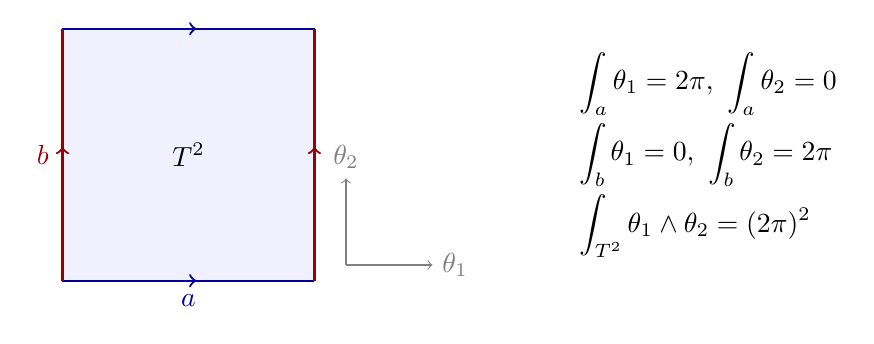
\begin{tikzpicture}[scale=1.0]
\draw[fill=blue!6] (0,0) rectangle (3.2,3.2);
\draw[->,thick,blue!60!black] (0,0) -- (1.7,0);
\draw[->,thick,blue!60!black] (0,3.2) -- (1.7,3.2);
\draw[blue!60!black,thick] (1.6,0) -- (3.2,0);
\draw[blue!60!black,thick] (1.6,3.2) -- (3.2,3.2);
\draw[->,thick,red!60!black] (0,0) -- (0,1.7);
\draw[->,thick,red!60!black] (3.2,0) -- (3.2,1.7);
\draw[red!60!black,thick] (0,1.6) -- (0,3.2);
\draw[red!60!black,thick] (3.2,1.6) -- (3.2,3.2);
\node[blue!60!black,below] at (1.6,-0.05) {$a$};
\node[red!60!black,left] at (-0.05,1.6) {$b$};
\node at (1.6,1.6) {$T^2$};
\draw[->,gray] (3.6,0.2) -- (4.7,0.2) node[right] {$\theta_1$};
\draw[->,gray] (3.6,0.2) -- (3.6,1.3) node[above] {$\theta_2$};
\node[align=left] at (8.2,1.6) {$\displaystyle\int_a\dd\theta_1=2\pi,\ \int_a\dd\theta_2=0$\\[2pt]
$\displaystyle\int_b\dd\theta_1=0,\ \int_b\dd\theta_2=2\pi$\\[2pt]
$\displaystyle\int_{T^2}\dd\theta_1\wedge\dd\theta_2=(2\pi)^2$};
\end{tikzpicture}
\caption{トーラス $T^2=\R^2/(2\pi\Z)^2$ の基本領域と2つの基本的な閉曲線 $a,b$。$[\dd\theta_1],[\dd\theta_2]$ は $a,b$ の上の積分で区別できる。}\label{B:fig:T2}
\end{figure}

\begin{ex}[$T^2$ の交叉形式]\label{B:ex:T2int}
$H^1(T^2)$ の基底 $[\dd\theta_1],[\dd\theta_2]$ と、$H^2(T^2)\cong\R$（$\int$）を使うと、$\alpha=p\,\dd\theta_1+q\,\dd\theta_2$, $\beta=r\,\dd\theta_1+s\,\dd\theta_2$ に対し
$\alpha\wedge\beta=(ps-qr)\,\dd\theta_1\wedge\dd\theta_2$、$\int_{T^2}\alpha\wedge\beta=(2\pi)^2(ps-qr)$。これは非退化な歪対称形式で、(iii) に一致する。
\end{ex}

\paragraph{部分多様体の双対（予告）。}向きづけられた閉部分多様体 $S^k\subset M^n$ に対し、$\int_S\iota^*\alpha=\int_M\alpha\wedge\eta_S$ $(\alpha\in\Om^k(M))$ を満たす閉形式 $\eta_S\in\Om^{n-k}(M)$（$S$ の Poincaré 双対）が、Poincaré 双対性から存在する。第6巻で、ベクトル束の切断の零点集合の双対が Chern 類になること（$c_k$ の幾何的意味）を見る。

\subsection{Künneth 公式・Euler 標数・連結和}\label{B:ss:kun}

\begin{thm}[Künneth]\label{B:thm:kunneth}\tC
$M$ が有限な良い被覆をもつなら、射影 $\mathrm{pr}_1,\mathrm{pr}_2:M\times N\to M,N$ に対し
\[
\bigoplus_{i+j=k}H^i(M)\otimes H^j(N)\xrightarrow{\ \cong\ }H^k(M\times N),\qquad[\alpha]\otimes[\beta]\mapsto[\mathrm{pr}_1^*\alpha\wedge\mathrm{pr}_2^*\beta].
\]
\end{thm}
\src{Bott--Tu 第I章 §5。MV と五項補題による。}
Betti 数の生成関数 $P_M(t)=\sum b_k(M)t^k$ は $P_{M\times N}=P_M\,P_N$ を満たし、$\chi(M\times N)=\chi(M)\chi(N)$。例：$P_{S^1}=1+t$ より $P_{T^n}=(1+t)^n$、すなわち $b_k(T^n)=\binom nk$、$\chi(T^n)=0$。$P_{S^2\times S^2}=(1+t^2)^2=1+2t^2+t^4$。

\paragraph{連結和。}$n$ 次元の多様体 $M,N$ から、点を中心とする小さな球 $D\subset M$, $D'\subset N$ を取り除き、境界の球面 $S^{n-1}$ を貼り合わせて得られる多様体を連結和（connected sum）$M\#N$ という（向きづけられた場合は向きが合うように貼る）。$S^2\#T^2=T^2$、$\Sigma_g=T^2\#\cdots\#T^2$（$g$ 個）。

\begin{prop}\label{B:prop:csum}\tP
$M,N$ を向きづけられた閉 $n$ 次元多様体とすると $\chi(M\#N)=\chi(M)+\chi(N)-2+\chi(S^{n-1})$。特に $n$ が偶数なら $\chi(M\#N)=\chi(M)+\chi(N)-2$。
\end{prop}
\begin{proof}
$M=(M\setminus\{p\})\cup D$ で $D$ は開球、$(M\setminus\{p\})\cap D\simeq S^{n-1}$。MV（命題~\ref{B:prop:chi}）より $\chi(M)=\chi(M\setminus\{p\})+1-\chi(S^{n-1})$（$D$ は可縮）。同様に $N$ でも。$M\#N=(M\setminus\{p\})\cup(N\setminus\{q\})$（開集合を少し広げて）で交わりは $S^{n-1}\times(-1,1)\simeq S^{n-1}$ だから $\chi(M\#N)=\chi(M\setminus\{p\})+\chi(N\setminus\{q\})-\chi(S^{n-1})=\bigl(\chi(M)-1+\chi(S^{n-1})\bigr)+\bigl(\chi(N)-1+\chi(S^{n-1})\bigr)-\chi(S^{n-1})$。（MV を使うとき、有限性は命題~\ref{B:prop:chi} の証明の議論で $M\setminus\{p\}$ について従う。）
\end{proof}
\begin{cor}[曲面の Betti 数]\label{B:cor:Sigma}\tP
種数 $g$ の向きづけられた閉曲面 $\Sigma_g$ は $\chi(\Sigma_g)=2-2g$、$(b_0,b_1,b_2)=(1,2g,1)$。
\end{cor}
\begin{proof}
$\chi(\Sigma_0)=\chi(S^2)=2$、$\Sigma_g=\Sigma_{g-1}\#T^2$ と $\chi(T^2)=0$、命題より $\chi(\Sigma_g)=\chi(\Sigma_{g-1})+0-2$。帰納法で $2-2g$。連結で向きづけられた閉曲面だから $b_0=b_2=1$（定理~\ref{B:thm:Hn}, \ref{B:thm:PD}）、よって $b_1=2-\chi=2g$。
\end{proof}
$\Sigma_g$ の同相型は $g$ だけで決まる（閉曲面の分類）\tC。向きづけ不可能な場合は $\RP^2\#\cdots\#\RP^2$（§2 で言及）。

\begin{ex}[射影空間：主張]\label{B:ex:proj}\tC
$H^k_{\rm dR}(\CP^n)\cong\R$（$k=0,2,\dots,2n$）、他は $0$。環としては $H^*(\CP^n)\cong\R[h]/(h^{n+1})$（$\deg h=2$）で、$h$ は $c_1(\mathcal O(1))$（§10）の類。$\RP^n$ は $n$ が奇数なら $b_0=b_n=1$、他は $0$、$n$ が偶数なら $b_0=1$、他は $0$（$\chi(\RP^n)=0$ または $1$）。（Bott--Tu 第I章 §5、Lee 第17章。$\RP^2$ は問~\ref{pr:B_chi}。）
\end{ex}

\subsection{de Rham の定理・{\Cech}--de Rham の予告}\label{B:ss:cech}

de Rham コホモロジーは実は位相的な量である。
\begin{thm}[de Rham の定理]\label{B:thm:dRthm}\tC
$H^k_{\rm dR}(M)\cong H^k_{\rm sing}(M;\R)$（特異コホモロジー）。この同型は $\omega\mapsto(\sigma\mapsto\int_\sigma\omega)$ で与えられ、環構造を保つ。
\end{thm}
\src{Lee 第18章、Bott--Tu 第II章（§8 以降の {\Cech}--de Rham 複体）、Warner 第5章。\tQ\ 節番号は未確認。}
したがって、Betti 数は多様体の滑らかな構造によらない。Chern 類を $H^{2k}(M;\Z)$ の元として考える（第6巻）ときの土台である。証明の道筋は第3巻で層のコホモロジーとして見る：$\underline{\R}\to\Om^0\to\Om^1\to\cdots$ は定数層の分解（Poincaré の補題が各点でこれの完全性を与える）であり、各 $\Om^k$ が（1の分割のおかげで）軟弱（fine）層であることから、$H^k_{\rm dR}(M)\cong H^k(M;\underline{\R})$ が従う。

\paragraph{{\Cech}--de Rham 複体の予告。}開被覆 $\mathcal U=\{U_\alpha\}$ に対し、二重複体 $C^{p}(\mathcal U,\Om^q)=\prod_{\alpha_0<\cdots<\alpha_p}\Om^q(U_{\alpha_0\cdots\alpha_p})$ に、{\Cech} 微分 $\delta$ と外微分 $\dd$ を考える。MV 列は、被覆が2個のときの {\Cech} 微分 $\delta$ に他ならない。「良い被覆」（有限交叉がすべて可縮）では、各 $U_{\alpha_0\cdots\alpha_p}$ に Poincaré の補題が使えて、この二重複体のコホモロジーが {\Cech} コホモロジー $\check H^p(\mathcal U;\R)$ に等しくなり、$H^k_{\rm dR}(M)\cong\check H^k(\mathcal U;\R)$ を得る（Bott--Tu 第II章）。第3巻では、$\Om^q$ を一般の層に置き換えて層コホモロジー理論を展開し、複素多様体の正則 de Rham 複体、Dolbeault 複体と結びつける。

\begin{keybox}{§5 の要点}
\begin{itemize}
\item $H^k_{\rm dR}=\Ker\dd/\Ran\dd$。反変関手で環構造をもつ。ホモトピー不変（Cartan の公式から出るホモトピー公式 $s_1^*-s_0^*=\dd K+K\dd$）。$\R^n$ は $H^0$ のみ（Poincaré の補題）。
\item 計算は Mayer--Vietoris（開被覆の貼り合わせ）：$H^*(S^n)=\R$ ($k=0,n$)、$H^*(T^n)=\Lambda^*\R^n$（$b_k=\binom nk$）、$\Sigma_g$ は $(1,2g,1)$、$\CP^n$ は $b_{2k}=1$。
\item 写像度：$\int_Mf^*\omega=\deg f\int_N\omega$。正則値の逆像の符号つき個数。$\deg(\text{対蹠写像})=(-1)^{n+1}$ から偶数次元球面の毛玉定理。
\item Poincaré 双対：向きづけられた閉 $n$ 次元で $H^k\times H^{n-k}\to\R$ が完全対。$b_k=b_{n-k}$、奇数次元で $\chi=0$。
\item \textbf{【あとで使う】}$H^k_{\rm dR}\cong H^k(M;\underline{\R})$ $\to$ 第3巻（層コホモロジー、{\Cech}--de Rham）。Poincaré 双対 $\to$ Serre 双対・統合論文の双対性（第4・5巻）。MV 列の連結準同型 $\to$ 長完全列の標準的な使い方。写像度・正則値 $\to$ 指数定理（第6巻）。
\end{itemize}
\end{keybox}

\paragraph{つまずきやすい点。}
\begin{enumerate}
\item \textbf{$H^k_{\rm dR}$ は位相不変量だが、$\dd$ は滑らかな構造に依存する。}代表元（閉形式）は微分同相でしか対応しない。ホモトピー同値、あるいは位相同型で不変なのは類だけ。
\item \textbf{Poincaré の補題は星状（可縮）の仮定が要る。}$\R^2\setminus\{0\}$ では閉形式 $\omega=\dd\theta$ が完全でない。「局所的には完全だが大域的には完全でない」という差が $H^1\ne0$ の意味で、局所と大域の間の障害を測るのがコホモロジーである。
\item \textbf{MV の符号。}$b(\mu,\nu)=\nu|_{U\cap V}-\mu|_{U\cap V}$ と取る流儀が多いが、$\mu-\nu$ の流儀もあり、$\delta$ の符号が変わる。同型を作るだけなら影響しないが、連結準同型の具体的な式を使うときは規約を確認する。
\item \textbf{Poincaré 双対は向きづけと連結性の仮定が必要。}非連結なら成分ごと、向きづけ不可能なら $H^n_{\rm dR}=0$（$\Z/2$ 係数なら成り立つ）。
\item \textbf{$H^k$ の次元は無限でありうる。}開多様体（例：$\R^2$ から可算無限個の点を除く）では $b_k=\infty$。Poincaré 双対の有限な良い被覆の仮定はこのためにある。
\end{enumerate}

\subsection*{問題（§5）}

\begin{probl}{標準}{B_primitive}
(a) $\R^3$ の $1$ 形式 $\alpha=y\,\dd x+x\,\dd y+2z\,\dd z$ が閉であることを確かめ、公式 \eqref{B:eq:Pformula} で原始関数を求めよ。(b) $\beta=x\,\dd y\wedge\dd z+y\,\dd z\wedge\dd x-2z\,\dd x\wedge\dd y$ が閉であることを確かめ、公式 \eqref{B:eq:Pformula}（$k=2$）で $\beta=\dd\gamma$ なる $1$ 形式 $\gamma$ を求め、$\dd\gamma=\beta$ を確かめよ。
\end{probl}

\begin{probl}{標準}{B_punct}
(a) $\R^2\setminus\{0\}$ 上の任意の閉 $1$ 形式 $\alpha$ は、ある定数 $c$ と関数 $f$ により $\alpha=c\,\omega+\dd f$（$\omega=\dd\theta$ は例~\ref{B:ex:angle} の角形式）と書け、$c=\frac1{2\pi}\oint_{S^1}\alpha$ であることを示せ。\hint{$i:S^1\hookrightarrow\R^2\setminus\{0\}$ が $H^1$ の同型を与える。}(b) $\R^2\setminus\{0\}$ 上のベクトル場 $\bs F=\dfrac{(-y,x)}{x^2+y^2}$ と $\bs G=\dfrac{(x,y)}{x^2+y^2}$ はどちらも rot $=0$ である。勾配場であるのはどちらか。理由とともに答えよ。
\end{probl}

\begin{probl}{標準}{B_S1MV}
$S^1=\R/2\pi\Z$ を $U=S^1\setminus\{\pi\}$, $V=S^1\setminus\{0\}$ で覆い、$U\cap V=W_1\sqcup W_2$（$W_1=(0,\pi)$, $W_2=(\pi,2\pi)$）とする。$\{\rho_U,\rho_V\}$ を従属する1の分割で、$\rho_U=1$ が $\theta=0$ の近く、$\rho_V=1$ が $\theta=\pi$ の近くであるものとする。$\tau\in H^0(U\cap V)$ が $W_1$ 上で定数 $\tau_1$、$W_2$ 上で定数 $\tau_2$ のとき、定理~\ref{B:thm:MV} の $\eta$ について $\int_{S^1}\eta=\tau_2-\tau_1$ を示し、$\delta\tau=\dfrac{\tau_2-\tau_1}{2\pi}[\dd\theta]$ を結論せよ。
\end{probl}

\begin{probl}{標準}{B_MVT2}
Mayer--Vietoris を用いて $T^2=S^1\times S^1$ の Betti 数が $(1,2,1)$ であることを示せ。\hint{$S^1=A\cup B$ を2つの開弧で覆い、$X=S^1\times A$, $Y=S^1\times B$ とおく。$X\cap Y\simeq S^1\sqcup S^1$。$H^1(X)\oplus H^1(Y)\to H^1(X\cap Y)$ の階数を調べる。}
\end{probl}

\begin{probl}{標準}{B_Rk}
$M_k=\R^2\setminus\{p_1,\dots,p_k\}$（$k$ 個の相異なる点）について、$\dim H^1(M_k)=k$, $H^2(M_k)=0$ を、$k$ に関する帰納法と Mayer--Vietoris で示せ。\hint{$D$ を $p_k$ を中心とし他の点を含まない小さな開円板として、$M_{k-1}=M_k\cup D$ に MV を適用する。}
\end{probl}

\begin{probl}{標準}{B_chi}
(a) 開 Möbius 帯は $S^1$ にホモトピー同値である（§2）ことを用いて、$\RP^2=(\text{開 Möbius 帯})\cup D$（$D$ は開円板、交わりは $S^1$ に同値な帯）に MV の加法性を使い、$\chi(\RP^2)=1$ を示せ。(b) $\chi(\Sigma_2)=-2$ を命題~\ref{B:prop:csum} から求め、$\chi(S^2\times\Sigma_2)$ と $\chi(T^3)$ を求めよ。(c) 連結で向きづけられた閉 $4$ 次元多様体 $M$ で $b_1=0$ ならば $\chi(M)=2+b_2$ であることを示せ。
\end{probl}

\begin{probl}{標準}{B_degree}
(a) $f_m(z)=z^m:S^1\to S^1$ の次数を $\int f_m^*\dd\theta$ と、正則値の逆像の個数の両方で求めよ（$m\in\Z$）。(b) $S^n$ の対蹠写像 $a$ は $n+1$ 個の鏡映 $r_i(x)=(x_0,\dots,-x_i,\dots,x_n)$ の合成であることを用い、$\deg a=(-1)^{n+1}$ を再確認せよ（鏡映の次数は $-1$）。(c) 有理関数 $f(z)=\dfrac{z^2+1}{z}$ を $\CP^1=S^2$ の自己写像（$f(0)=f(\infty)=\infty$）と見たときの次数を求めよ。
\end{probl}

\begin{probl}{発展}{B_brouwer}
(a) 滑らかな写像 $r:D^2\to S^1=\partial D^2$ で $r|_{S^1}=\id$ となるものは存在しないことを、$r^*\dd\theta$ に Stokes の定理を使って示せ。(b) 滑らかな写像 $g:D^2\to D^2$ は不動点をもつことを (a) から示せ。
\end{probl}


\begin{probl}{標準}{B_PD}
(a) 連結で向きづけられた閉 $3$ 次元多様体では $b_1=b_2$ かつ $\chi=0$ であることを示せ。(b) $S^1\times S^2$, $T^3$, $T^4$, $S^2\times S^2$ の Betti 数と Euler 標数を Künneth の公式で求め、Poincaré 双対性の対称性 $b_k=b_{n-k}$ を確かめよ。(c) 向きづけられた閉曲面で $b_1$ は偶数であることを、対 $H^1\times H^1\to\R$ から示せ。
\end{probl}

\begin{probl}{標準}{B_kun}
$\sigma\in\Om^2(S^2)$ を $\int_{S^2}\sigma=1$ なる $2$ 形式とし、$a=[\mathrm{pr}_1^*\sigma]$, $b=[\mathrm{pr}_2^*\sigma]\in H^2(S^2\times S^2)$ とする。(a) $a,b$ が $H^2$ の基底であること（Künneth）を使い、$a^2=b^2=0$、$ab$ は $H^4$ の生成元（$\int ab=1$）であることを示せ。(b) 対 $H^2\times H^2\to\R$ の行列を $(a,b)$ 基底で求め、非退化であること、不定符号であることを確かめよ。
\end{probl}

\begin{probl}{発展}{B_Hc}
$M=\R^2\setminus\{0\}$ とし、$\varphi\in C^\infty(\R)$ を $r\le1$ で $0$、$r\ge2$ で $1$ とする。(a) $\eta=\varphi'(r)\,\dd r$ は $M$ 上のコンパクト台の閉 $1$ 形式であることを示せ。(b) $\eta$ は $\Om^1_c(M)$ の中で完全でない（$\eta=\dd g$, $g\in C^\infty_c(M)$ とはならない）ことを示せ。(c) $\int_M\omega\wedge\eta$（$\omega=\dd\theta$）を計算し、Poincaré 双対の対 $H^1(M)\times H^1_c(M)\to\R$ が非自明であることを確かめよ。
\end{probl}

\begin{probl}{標準}{B_div3}
$\R^3\setminus\{0\}$ 上の $\omega=\dfrac{x\,\dd y\wedge\dd z+y\,\dd z\wedge\dd x+z\,\dd x\wedge\dd y}{(x^2+y^2+z^2)^{3/2}}$ について、(a) $\dd\omega=0$ を示せ。(b) 半径 $\rho$ の球面 $S_\rho$（外向き法線先頭の向き）で $\int_{S_\rho}\omega=4\pi$ を示せ。(c) 原点を内部に含む任意のコンパクトな滑らかな境界をもつ領域 $\Omega$ に対し $\int_{\partial\Omega}\omega=4\pi$ を示し、$\omega$ が完全でないことを結論せよ（点電荷に対する Gauss の法則）。
\end{probl}

%==================================================
\section{Riemann 計量・Hodge 星・Laplacian}\label{B:sec6}
%==================================================

\begin{goalbox}{この節のねらい}
微分形式の理論（§4--5）では、$\dd$, $\wedge$, $\int$ は計量なしに定義できた。しかし「長さ」「角度」「体積」や、「$\dd$ の随伴」「Laplacian」には Riemann 計量が要る。(1) Riemann 計量と体積形式、(2) 形式の内積と Hodge 星 $\star$（$\R^3$, $\R^4$ の表）、(3) 随伴 $\delta$ と Hodge Laplacian、(4) Hodge の定理（コンパクト多様体：主張と出典、トーラス上では完全な証明）、(5) 共形不変性と $\R^4$ の自己双対・反自己双対分解（ゲージ理論への伏線）、を学ぶ。前提：§4, §5。Levi-Civita 接続は §8 で扱う。
\end{goalbox}

\subsection{Riemann 計量}\label{B:ss:metric}

多様体上の点における接ベクトルの長さや、2つのベクトルのなす角を測りたい。Euclid 空間では内積が使えるが、一般の多様体には $\R^n$ の標準内積が「どれ」と決まっていないので、各接空間に内積を「付け加える」必要がある。

\begin{defn}[Riemann 計量]\label{B:def:metric}
多様体 $M$ の Riemann 計量（Riemannian metric）$g$ とは、各 $T_pM$ 上の内積（対称・正定値な双線形形式）$g_p$ で、$p$ について滑らかなもの（すなわち $g(X,Y)\in C^\infty(M)$ がすべての $X,Y\in\X(M)$ について成り立つ）をいう。組 $(M,g)$ を Riemann 多様体という。座標では $g=g_{ij}\,\dd x^i\dd x^j$、$g_{ij}=g(\pa_i,\pa_j)$（対称正定値行列）で、$g^{ij}$ で逆行列を表す。
\end{defn}

\begin{prop}[存在]\label{B:prop:gexist}\tP
任意の多様体は Riemann 計量をもつ。
\end{prop}
\begin{proof}
座標近傍 $(U_\alpha,x_\alpha)$ の開被覆と従属する1の分割 $\{\rho_\alpha\}$（局所有限）をとる。各 $U_\alpha$ 上に $g_\alpha=\sum_i(\dd x^i_\alpha)^2$（標準計量の引き戻し）をおき、$g=\sum_\alpha\rho_\alpha g_\alpha$ とする（$\rho_\alpha g_\alpha$ は $U_\alpha$ の外に $0$ で延長して滑らか）。各点で $g_p$ は対称で、$\rho_\alpha(p)\ge0$ かつ和が $1$ だから、正定値な $g_\alpha(p)$ の凸結合として正定値。
\end{proof}
（これは §7 のファイバー計量の存在と同じ論法である。）

\begin{ex}[例]\label{B:ex:metric}
(1) $\R^n$ の標準計量 $g=\sum(\dd x^i)^2$。(2) $M\subset\R^N$ が部分多様体なら、誘導計量 $\iota^*g_{\rm Euc}$ が入る。例えば $S^2\subset\R^3$ の球面座標 $\Phi(\theta,\varphi)=(\sin\theta\cos\varphi,\sin\theta\sin\varphi,\cos\theta)$ では $\Phi_\theta=(\cos\theta\cos\varphi,\cos\theta\sin\varphi,-\sin\theta)$, $\Phi_\varphi=(-\sin\theta\sin\varphi,\sin\theta\cos\varphi,0)$ で $|\Phi_\theta|^2=1$, $\Phi_\theta\cdot\Phi_\varphi=0$, $|\Phi_\varphi|^2=\sin^2\theta$ だから
\[
g_{S^2}=\dd\theta^2+\sin^2\theta\,\dd\varphi^2 .
\]
(3) トーラス $T^n=\R^n/(2\pi\Z)^n$ は $\sum(\dd x^i)^2$ が平行移動で不変だから、平坦計量が入る。(4) 上半平面 $\{y>0\}$ の $g=(\dd x^2+\dd y^2)/y^2$（双曲計量）。(5) 積 $M\times N$ の計量 $g_M\oplus g_N$。
\end{ex}

\paragraph{長さと体積。}曲線 $\gamma:[a,b]\to M$ の長さは $L(\gamma)=\int_a^b\sqrt{g(\dot\gamma,\dot\gamma)}\,\dd t$（パラメータのとり方によらない）。向きづけられた $(M,g)$ には、体積形式（volume form）$\Bvol_g\in\Om^n(M)$ が定まる：正の向きの正規直交基底 $(e_1,\dots,e_n)$ に対し $\Bvol_g(e_1,\dots,e_n)=1$。座標では
\begin{equation}\label{B:eq:volg}
\Bvol_g=\sqrt{\det(g_{ij})}\,\dd x^1\wedge\cdots\wedge\dd x^n\qquad(\text{正の向きの座標}).
\end{equation}
\begin{proof}[式~\eqref{B:eq:volg} の確認]
$e_a=A^i_a\pa_i$（$A$ は正の向きなので $\det A>0$）が正規直交なら $\delta_{ab}=g(e_a,e_b)=A^i_ag_{ij}A^j_b$、$\det(A)^2\det g=1$、$\det A=1/\sqrt{\det g}$。$(\sqrt{\det g}\,\dd x^1\wedge\cdots)(e_1,\dots,e_n)=\sqrt{\det g}\det A=1$。
\end{proof}
$S^2$ では $\sqrt{\det g}=\sin\theta$ で $\Bvol_g=\sin\theta\,\dd\theta\wedge\dd\varphi$、面積 $\int_{S^2}\Bvol_g=4\pi$（問~\ref{pr:B_sphere} の $\Phi^*\omega$ と一致する：$\omega|_{S^2}=\Bvol_g$）。計量は体積 $\mathrm{Vol}(M)=\int_M\Bvol_g$ を定め、これは $M$ が向きづけられていなくても測度として意味をもつ。

\paragraph{$\flat$ と $\sharp$。}計量は $T_pM\cong T_p^*M$ を与える：$v^\flat=g(v,\cdot)$, $\xi^\sharp=(\flat)^{-1}\xi$。座標では $v^\flat=g_{ij}v^j\,\dd x^i$, $\xi^\sharp=g^{ij}\xi_j\pa_i$。関数の勾配は $\Bgrad f=(\dd f)^\sharp$。§1 の $V\cong V^*$ の多様体版である。一方、$T\oplus T^*$ の自然な符号 $(n,n)$ の内積（§1）は計量なしで定義され、計量を使うと $\flat$ が $T\oplus T^*$ の中の「$g$ のグラフ」を与える（Courant 代数・一般化複素幾何の巻）。

\begin{figure}[ht]
\centering
\begin{tikzpicture}[scale=1.0]
% left: unit circle in coordinate basis = ellipse
\begin{scope}
\draw[->,gray] (-2.3,0) -- (2.4,0) node[right] {\small $\pa_1$};
\draw[->,gray] (0,-2.0) -- (0,2.2) node[above] {\small $\pa_2$};
\begin{scope}[rotate=25]
\draw[thick,blue!60!black] (0,0) ellipse (1.7 and 0.9);
\end{scope}
\node[blue!60!black] at (2.0,1.55) {$\{g(v,v)=1\}$};
\draw[->,thick,red!60!black] (0,0) -- (1.3,0.6) node[above right] {$v$};
\node at (0,-2.7) {$T_pM$：単位球は楕円（座標が正規直交でないとき）};
\end{scope}
% right: area element
\begin{scope}[xshift=7cm]
\fill[orange!25] (0,0) -- (2.0,0) -- (2.6,1.5) -- (0.6,1.5) -- cycle;
\draw[->,thick] (0,0) -- (2.0,0) node[below right] {$\pa_1$};
\draw[->,thick] (0,0) -- (0.6,1.5) node[above left] {$\pa_2$};
\draw[dashed] (2.0,0) -- (2.6,1.5) -- (0.6,1.5);
\node at (1.3,0.75) {$\sqrt{\det g}$};
\node at (1.1,-1.2) {$\Bvol_g(\pa_1,\pa_2)=\sqrt{\det g}$};
\node at (1.1,-1.7) {（$\pa_1,\pa_2$ が張る平行四辺形の面積）};
\end{scope}
\end{tikzpicture}
\caption{計量は各接空間に「単位球」と「面積」を与える。座標基底が正規直交でないとき、$\Bvol_g(\pa_1,\dots,\pa_n)=\sqrt{\det g}$。}\label{B:fig:metric}
\end{figure}

\begin{figure}[ht]
\centering
\begin{tikzpicture}[scale=1.15]
\draw[thick] (0,0) circle (1.6);
\foreach \yy/\rr/\qq in {1.386/0.8/0.224, 0.8/1.386/0.388, 0/1.6/0.448, -0.8/1.386/0.388, -1.386/0.8/0.224} {
  \draw[gray!60] (-\rr,\yy) arc[start angle=180,end angle=360,x radius=\rr,y radius=\qq];
  \draw[gray!60,dashed] (-\rr,\yy) arc[start angle=180,end angle=0,x radius=\rr,y radius=\qq];
}
\draw[gray!60] (0,-1.6) .. controls (0.9,-1.2) and (1.35,-0.6) .. (1.6,0);
\draw[gray!60] (0,1.6) .. controls (0.9,1.2) and (1.35,0.6) .. (1.6,0);
\draw[gray!60] (0,-1.6) .. controls (-0.9,-1.2) and (-1.35,-0.6) .. (-1.6,0);
\draw[gray!60] (0,1.6) .. controls (-0.9,1.2) and (-1.35,0.6) .. (-1.6,0);
% small patch
\fill[orange!50,opacity=0.7] (0.75,0.8) -- (1.05,0.78) -- (1.1,0.35) -- (0.75,0.36) -- cycle;
\draw[thick,red!60!black] (0.75,0.8) -- (1.05,0.78) -- (1.1,0.35) -- (0.75,0.36) -- cycle;
\fill (0,1.6) circle (1.5pt);
\node[above] at (0,1.62) {$N$（$\theta=0$）};
\draw[->,thick,blue!60!black] (2.3,0.35) -- (2.3,0.9) node[right] {$\theta$ 増};
\draw[->,thick,blue!60!black] (2.3,0.35) -- (3.0,0.35) node[right] {$\varphi$ 増};
\node[align=left,anchor=west] at (3.0,-0.7) {小さな四角形の面積\\ $\approx\sin\theta\,\dd\theta\,\dd\varphi$};
\end{tikzpicture}
\caption{$S^2$ の球面座標。座標線（緯線・経線）が作る小さな四角形の辺は $\dd\theta$ と $\sin\theta\,\dd\varphi$ で、面積要素 $\sin\theta\,\dd\theta\wedge\dd\varphi$ を与える。}\label{B:fig:S2coord}
\end{figure}

\subsection{形式の内積と Hodge 星}\label{B:ss:star}

$\dim\Lambda^kV^*=\binom nk=\dim\Lambda^{n-k}V^*$ である。内積と向きがあれば、この2つの空間の間に自然な同型を作ることができる。これが Hodge 星作用素である。電磁気学で「電場 $\bs E$ ↔ 2 形式」「磁場 $\bs B$ ↔ 2 形式」と同一視を行き来するときに使われている構造である。

\paragraph{$\Lambda^kV^*$ の内積。}$(V,\langle\,,\rangle)$ を向きづけられた $n$ 次元内積空間とする。$V^*$ には $\flat,\sharp$ を通じて内積が入る。$\Lambda^kV^*$ の内積を
\[
\langle\alpha^1\wedge\cdots\wedge\alpha^k,\ \beta^1\wedge\cdots\wedge\beta^k\rangle=\det\bigl(\langle\alpha^i,\beta^j\rangle\bigr)
\]
で定める。$(e^1,\dots,e^n)$ が $V^*$ の正規直交基底ならば $\{e^I=e^{i_1}\wedge\cdots\wedge e^{i_k}\}_{i_1<\cdots<i_k}$ は $\Lambda^kV^*$ の正規直交基底（行列式の値が $\delta_{IJ}$ になる）。$\Bvol=e^1\wedge\cdots\wedge e^n$ を体積形式とする（正の向きの正規直交余基底）。

\begin{defn}[Hodge 星]\label{B:def:star}
$\star:\Lambda^kV^*\to\Lambda^{n-k}V^*$ を、すべての $\alpha,\beta\in\Lambda^kV^*$ に対し
\[
\alpha\wedge\star\beta=\langle\alpha,\beta\rangle\,\Bvol
\]
が成り立つものとして定める。
\end{defn}

\begin{prop}[Hodge 星の性質]\label{B:prop:star}\tP
(i) $\star$ は一意に存在し、正の向きの正規直交余基底 $(e^i)$ に関して $\star e^I=\Bsgn(I,I^c)\,e^{I^c}$（$I^c$ は補集合を昇順に並べたもの、$\Bsgn(I,I^c)$ は並べ $(I,I^c)$ の符号、すなわち $e^I\wedge e^{I^c}=\Bsgn(I,I^c)\Bvol$）。(ii) $\star1=\Bvol$, $\star\Bvol=1$。(iii) $\star\star=(-1)^{k(n-k)}$ on $\Lambda^k$。(iv) $\langle\star\alpha,\star\beta\rangle=\langle\alpha,\beta\rangle$（等長）。(v) $\alpha\wedge\star\beta=\beta\wedge\star\alpha$。
\end{prop}
\begin{proof}
(i) $\alpha=e^I$ とし、$\star e^K=\sum_Jc^K_Je^J$ とおくと、定義は $e^I\wedge\star e^K=\delta_{IK}\Bvol$。$e^I\wedge e^J\ne0$ となるのは $J=I^c$ のときだけで、そのとき値は $\Bsgn(I,I^c)\Bvol$。したがって $\star e^K$ の係数は $J=K^c$ 以外は $0$、$J=K^c$ では $c^K_{K^c}\Bsgn(K,K^c)=1$、すなわち $c=\Bsgn(K,K^c)$。これは存在と一意性を与える。(ii) は $k=0,n$ の場合の (i)。(iii) $\star\star e^K=\Bsgn(K,K^c)\star e^{K^c}=\Bsgn(K,K^c)\Bsgn(K^c,K)e^K$ で、並べ $(K^c,K)$ と $(K,K^c)$ は $k(n-k)$ 回の互換で移り合うので $\Bsgn(K^c,K)=(-1)^{k(n-k)}\Bsgn(K,K^c)$。(iv)(v) は (i) と、$\alpha\wedge\star\beta=\langle\alpha,\beta\rangle\Bvol$ の対称性から。
\end{proof}
多様体上では、各点で上を適用して $\star:\Om^k(M)\to\Om^{n-k}(M)$ を得る（向きづけられた Riemann 多様体）。滑らかな形式を滑らかな形式に写す。内積 $\langle\alpha,\beta\rangle=\sum_I\alpha_I\beta_I$（正規直交余基底に関して）は $C^\infty$ 関数を与える。

\begin{ex}[$\R^3$ の Hodge 星]\label{B:ex:star3}
標準計量と標準の向き。$\star1=\dd x\wedge\dd y\wedge\dd z$ で、
\[
\star\dd x=\dd y\wedge\dd z,\quad\star\dd y=\dd z\wedge\dd x,\quad\star\dd z=\dd x\wedge\dd y,
\]
\[
\star(\dd y\wedge\dd z)=\dd x,\quad\star(\dd z\wedge\dd x)=\dd y,\quad\star(\dd x\wedge\dd y)=\dd z,\quad\star\Bvol=1 .
\]
$\star\star=1$（$k(3-k)$ は常に偶数）。これを使うと、ベクトル解析は次のように書ける（$\bs F=(P,Q,R)$, $\bs F^\flat=P\,\dd x+Q\,\dd y+R\,\dd z$）：
\[
(\Bcurl\bs F)^\flat=\star\dd\bs F^\flat,\qquad\Bdiv\bs F=\star\dd\star\bs F^\flat,\qquad(\bs a\times\bs b)^\flat=\star(\bs a^\flat\wedge\bs b^\flat).
\]
実際、$\star\bs F^\flat=P\,\dd y\wedge\dd z+Q\,\dd z\wedge\dd x+R\,\dd x\wedge\dd y$ に \S\ref{B:ss:vec} の公式 $\dd(\cdots)=(P_x+Q_y+R_z)\Bvol$ を使えば第2式、$\dd\bs F^\flat$ に $\star$ を作用させれば第1式（\S\ref{B:ss:vec} の $\dd\bs F^\flat$ の式で $\dd y\wedge\dd z\mapsto\dd x$ などと置き換える）、第3式は外積の表（§4）から。第1式から $\dd\dd f=0$ が $\Bcurl\Bgrad=0$ に、第2式から $\dd\dd=0$ が $\Bdiv\Bcurl=0$ に対応する。
\end{ex}

\begin{ex}[$\R^4$ の Hodge 星]\label{B:ex:star4}
座標 $(x^1,\dots,x^4)$、$\Bvol=\dd x^1\wedge\dd x^2\wedge\dd x^3\wedge\dd x^4$、$\dd x^{ij}=\dd x^i\wedge\dd x^j$ などと略記する。命題~\ref{B:prop:star}(i) から
\begin{center}
\small
\begin{tabular}{@{}lll@{}}
\toprule
$k=1$ & $k=2$ & $k=3$ \\
\midrule
$\star\dd x^1=\dd x^{234}$ & $\star\dd x^{12}=\dd x^{34}$ & $\star\dd x^{123}=\dd x^4$ \\
$\star\dd x^2=-\dd x^{134}$ & $\star\dd x^{13}=-\dd x^{24}$ & $\star\dd x^{124}=-\dd x^3$ \\
$\star\dd x^3=\dd x^{124}$ & $\star\dd x^{14}=\dd x^{23}$ & $\star\dd x^{134}=\dd x^2$ \\
$\star\dd x^4=-\dd x^{123}$ & $\star\dd x^{23}=\dd x^{14}$ & $\star\dd x^{234}=-\dd x^1$ \\
 & $\star\dd x^{24}=-\dd x^{13}$ & \\
 & $\star\dd x^{34}=\dd x^{12}$ & \\
\bottomrule
\end{tabular}
\end{center}
（$k(4-k)=3,4,3$ なので $\star\star=-1,+1,-1$。例：$\star\star\dd x^1=\star\dd x^{234}=-\dd x^1$ ✓。）
\end{ex}

\paragraph{共形変換。}計量を $\tilde g=e^{2u}g$（$u\in C^\infty(M)$）に取り替える。正規直交余基底 $(e^i)$ は $\tilde e^i=e^ue^i$ に変わる。(i) より $\tilde\star\tilde e^I=\Bsgn\,\tilde e^{I^c}$、$\tilde e^I=e^{ku}e^I$ だから
\begin{equation}\label{B:eq:starconf}
\tilde\star=e^{(n-2k)u}\star\quad\text{on }\Om^k.
\end{equation}
特に $n=2k$（中次元の形式）では $\star$ が共形不変（$e^{2u}$ によらない）。$n=2$ の $1$ 形式、$n=4$ の $2$ 形式がその典型である（\S\ref{B:ss:conf}）。

\subsection{随伴 $\delta$ と Hodge Laplacian}\label{B:ss:delta}

向きづけられたコンパクトな Riemann 多様体 $(M,g)$ 上で、形式の $L^2$ 内積を
\[
(\alpha,\beta)=\int_M\alpha\wedge\star\beta=\int_M\langle\alpha,\beta\rangle\,\Bvol_g\qquad(\alpha,\beta\in\Om^k(M))
\]
で定める。これは対称で、$(\alpha,\alpha)=0\Rightarrow\alpha=0$（正定値）。$\dd$ の随伴を求めたい。

\begin{prop}[$\dd$ の随伴]\label{B:prop:delta}\tP
$\delta:\Om^k(M)\to\Om^{k-1}(M)$ を $\delta=(-1)^{n(k+1)+1}\star\dd\star$ で定めると、$M$ が閉（コンパクトで境界なし）のとき、すべての $\alpha\in\Om^{k-1}$, $\beta\in\Om^k$ について
\[
(\dd\alpha,\beta)=(\alpha,\delta\beta).
\]
同じことだが、$\delta=(-1)^k\star^{-1}\dd\star$ on $\Om^k$。
\end{prop}
\begin{proof}
$\dd(\alpha\wedge\star\beta)=\dd\alpha\wedge\star\beta+(-1)^{k-1}\alpha\wedge\dd\star\beta$（$\alpha\in\Om^{k-1}$）。Stokes（系~\ref{B:cor:exactint}）より左辺の積分は $0$ だから $(\dd\alpha,\beta)=(-1)^k\int_M\alpha\wedge\dd\star\beta$。$\dd\star\beta\in\Om^{n-k+1}$ を $\star(\star^{-1}\dd\star\beta)$ と書き、$\star^{-1}\dd\star\beta\in\Om^{k-1}$ だから、定義 $\alpha\wedge\star\gamma=\langle\alpha,\gamma\rangle\Bvol$ により $(\dd\alpha,\beta)=(-1)^k(\alpha,\star^{-1}\dd\star\beta)$。よって $\delta=(-1)^k\star^{-1}\dd\star$。$\star^{-1}$ は $j=n-k+1$ 次の形式に対して $(-1)^{j(n-j)}\star$（命題~\ref{B:prop:star}(iii)）なので $\delta=(-1)^{k+(n-k+1)(k-1)}\star\dd\star$。指数は mod 2 で $k+n(k-1)+(k-1)\equiv n(k+1)+1$（$(k-1)^2\equiv k-1$ を使った）。
\end{proof}
符号は文献により異なる（$\delta$ を $-(\ldots)$ に取る流儀や、$\dd^*$ と書く流儀がある）。ここでは $\delta$ が $\dd$ の（形式的）随伴であることから決めた。

\begin{ex}[$\R^n$ の標準計量での $\delta$]\label{B:ex:deltaR}
$\R^n$（またはトーラス）で $\dd=\sum_j\dd x^j\wedge\pa_j$ と見る。ここで $\dd x^j\wedge$ は各点での外積演算子で、その随伴（各点で $\Lambda^*$ の標準内積に関する）は $\iota_{\pa_j}$（$\{e^I\}$ が正規直交なので、$e^j\wedge e^I$ と $e^K$ の内積を比べればよい）、$\pa_j$ の $L^2$ 随伴は部分積分で $-\pa_j$ だから
\begin{equation}\label{B:eq:deltaflat}
\delta=-\sum_{j=1}^n\iota_{\pa_j}\pa_j .
\end{equation}
1形式 $f_i\dd x^i$ では $\delta(f_i\,\dd x^i)=-\sum_i\pa_if_i=-\Bdiv\bs f$。$\R^3$ の $2$ 形式では、$\delta=(-1)^{3\cdot3+1}\star\dd\star=\star\dd\star$ で、$\star\dd\star(a\,\dd y\wedge\dd z+b\,\dd z\wedge\dd x+c\,\dd x\wedge\dd y)=(\Bcurl(a,b,c))^\flat$（問~\ref{pr:B_adj}）。
\end{ex}

\begin{defn}[Hodge Laplacian、調和形式]\label{B:def:Hodge}
$\Delta=\dd\delta+\delta\dd:\Om^k(M)\to\Om^k(M)$ を Hodge Laplacian という。$\Delta\alpha=0$ なる $\alpha$ を調和形式（harmonic form）、その空間を $\mathcal H^k(M)$ と書く。
\end{defn}

\begin{prop}\label{B:prop:Lap}\tP
$M$ が向きづけられた閉 Riemann 多様体のとき：(i) $(\Delta\alpha,\beta)=(\alpha,\Delta\beta)$（自己随伴）、(ii) $(\Delta\alpha,\alpha)=\|\dd\alpha\|^2+\|\delta\alpha\|^2\ge0$、(iii) $\Delta\alpha=0\iff\dd\alpha=0$ かつ $\delta\alpha=0$（閉かつ余閉）、(iv) $\alpha\in\mathcal H^k\iff\star\alpha\in\mathcal H^{n-k}$。
\end{prop}
\begin{proof}
(i)(ii) は $(\dd\delta\alpha,\beta)=(\delta\alpha,\delta\beta)=(\alpha,\dd\delta\beta)$ と $(\delta\dd\alpha,\beta)=(\dd\alpha,\dd\beta)=(\alpha,\delta\dd\beta)$ から。(iii) ($\Leftarrow$) は明らか。($\Rightarrow$) $0=(\Delta\alpha,\alpha)=\|\dd\alpha\|^2+\|\delta\alpha\|^2$。(iv) $\delta\alpha=\pm\star^{-1}\dd\star\alpha$ だから $\delta\alpha=0\iff\dd(\star\alpha)=0$、また $\delta(\star\alpha)=\pm\star^{-1}\dd\star\star\alpha=\pm\star^{-1}\dd\alpha$ だから $\dd\alpha=0\iff\delta(\star\alpha)=0$。したがって (iii) より $\alpha$ が調和 $\iff\alpha$ が閉かつ余閉 $\iff\star\alpha$ が閉かつ余閉 $\iff\star\alpha$ が調和。
\end{proof}

\paragraph{関数に対する Laplacian。}$f\in C^\infty(M)$ では $\delta f=0$ で $\Delta f=\delta\dd f=(-1)^{2n+1}\star\dd\star\dd f=-\star\dd\star\dd f$。$1$ 形式 $\alpha$ に対し $\star\alpha=\iota_{\alpha^\sharp}\Bvol_g$ である（$\beta\wedge\iota_X\Bvol=\beta(X)\Bvol$ と $\beta(\alpha^\sharp)=\langle\beta,\alpha\rangle$ から）。したがって $\star\dd f=\iota_{\Bgrad f}\Bvol_g$ で、式~\eqref{B:eq:volg} を用いると $\iota_X\Bvol_g=\sqrt{\det g}\sum_i(-1)^{i-1}X^i\,\dd x^1\wedge\cdots\widehat{\dd x^i}\cdots\wedge\dd x^n$、$\dd\iota_X\Bvol_g=\sum_i\pa_i(\sqrt{\det g}\,X^i)\,\dd x^1\wedge\cdots\wedge\dd x^n$ だから（$\star(\dd x^1\wedge\cdots\wedge\dd x^n)=1/\sqrt{\det g}$）
\begin{equation}\label{B:eq:laplacefn}
\Delta f=-\frac1{\sqrt{\det g}}\sum_{i,j}\frac{\pa}{\pa x^i}\Bigl(\sqrt{\det g}\,g^{ij}\frac{\pa f}{\pa x^j}\Bigr)=-\Bdiv\Bgrad f .
\end{equation}
符号は、$\Delta$ が非負（$\Delta\ge0$）であるように決めた（幾何学者の Laplacian。解析学では $\sum\pa_i^2$ を $\Delta$ と書くので、符号が逆）。

\begin{ex}[具体例]\label{B:ex:lap}
(1) $\R^n$：$\Delta f=-\sum\pa_i^2f$。(2) $\R^2$ の極座標：$g=\dd r^2+r^2\dd\theta^2$、$\sqrt{\det g}=r$、$g^{rr}=1,g^{\theta\theta}=r^{-2}$ で
$\Delta f=-\frac1r\pa_r(r\pa_rf)-\frac1{r^2}\pa_\theta^2f$。調和関数は $\log r,\ r^k\cos k\theta,\ r^k\sin k\theta$ など。(3) $S^2$：$g=\dd\theta^2+\sin^2\theta\,\dd\varphi^2$、$\sqrt{\det g}=\sin\theta$ で
$\Delta f=-\frac1{\sin\theta}\pa_\theta(\sin\theta\,\pa_\theta f)-\frac1{\sin^2\theta}\pa_\varphi^2f$。$f=\cos\theta$ で $\pa_\theta f=-\sin\theta$, $\pa_\theta(-\sin^2\theta)=-2\sin\theta\cos\theta$ だから $\Delta\cos\theta=2\cos\theta$。同様に $\Delta(\sin\theta\,e^{i\varphi})=2\sin\theta\,e^{i\varphi}$。これらは $z,x+iy$ の $S^2$ への制限で、固有値 $\ell(\ell+1)=2$ （$\ell=1$ の球面調和関数）である（問~\ref{pr:B_lap}）。$S^2$ 上の調和関数は定数だけ（(ii)(iii) から $\dd f=0$）で $b_0=1$ と整合する。
\end{ex}

\subsection{Hodge の定理}\label{B:ss:HodgeThm}

de Rham コホモロジーの元（閉形式の類）には、代表元の選び方に任意性がある。計量を入れると、その中から「もっとも良い」ものを選ぶことができる。それが調和形式である。

\begin{thm}[Hodge の定理]\label{B:thm:Hodge}\tC
$(M,g)$ を向きづけられたコンパクトな（境界のない）Riemann 多様体とする。
\begin{enumerate}[label=(\roman*)]
\item $\mathcal H^k(M)=\Ker\Delta$ は有限次元。
\item $L^2$ 直交分解（Hodge 分解）
\[
\Om^k(M)=\mathcal H^k(M)\oplus\dd\Om^{k-1}(M)\oplus\delta\Om^{k+1}(M)
\]
が成り立つ。
\item したがって、各コホモロジー類は調和形式をちょうど1つだけ含む：$\mathcal H^k(M)\to H^k_{\rm dR}(M)$, $h\mapsto[h]$ は同型。特に $b_k<\infty$。
\end{enumerate}
\end{thm}
\src{Warner 第6章（Hodge の定理の完全な証明：Laplacian の楕円型正則性と Fredholm 的な議論）。証明の核心は $\Delta$ の楕円性で、これを使って $\Delta$ が（コンパクト多様体上で）有限次元の核と閉像をもつことを示す。この巻では、トーラスの場合に限って完全に証明する（次小節）。}

\paragraph{分解からコホモロジーとの同型を導く。}(ii) を認める。直交性は易しい：$(\dd\alpha,\delta\beta)=(\dd\dd\alpha,\beta)=0$、$h\in\mathcal H^k$ なら $\dd h=0=\delta h$ （命題~\ref{B:prop:Lap}(iii)）より $(h,\dd\alpha)=(\delta h,\alpha)=0$, $(h,\delta\beta)=(\dd h,\beta)=0$。閉形式 $\omega=h+\dd\alpha+\delta\beta$ をとると $0=\dd\omega=\dd\delta\beta$ だから $\|\delta\beta\|^2=(\beta,\dd\delta\beta)=0$。したがって閉形式は $\omega=h+\dd\alpha$ と書け、$[\omega]=[h]$：$\mathcal H^k\to H^k$ は全射。単射：$h=\dd\eta$ なら $\|h\|^2=(h,\dd\eta)=(\delta h,\eta)=0$。よって (iii)。

\begin{cor}[Hodge 星と Poincaré 双対]\label{B:cor:HodgePD}\tP
定理~\ref{B:thm:Hodge} のもとで $\star:\mathcal H^k\to\mathcal H^{n-k}$ は同型（命題~\ref{B:prop:Lap}(iv)）、したがって $b_k=b_{n-k}$。また $\mathcal H^k\times\mathcal H^{n-k}\to\R$, $(\alpha,\beta)\mapsto\int\alpha\wedge\beta$ は、$\int\alpha\wedge\star\alpha=\|\alpha\|^2>0$ により非退化である。これは Poincaré 双対（定理~\ref{B:thm:PD}）の別証明を与える（ただし Hodge の定理を使う）。
\end{cor}

\begin{cor}[調和形式の最小性]\label{B:cor:minim}\tP
閉形式 $\omega=h+\dd\eta$（$h$ は調和）に対し $\|\omega\|^2=\|h\|^2+\|\dd\eta\|^2\ge\|h\|^2$。すなわち調和形式は、その類の中で $L^2$ ノルムが最小の代表元である。
\end{cor}
\begin{proof}
$(h,\dd\eta)=(\delta h,\eta)=0$ だから、$\|h+\dd\eta\|^2=\|h\|^2+\|\dd\eta\|^2$。
\end{proof}

\begin{figure}[ht]
\centering
\begin{tikzpicture}[scale=1.0]
\draw[blue!60!black,very thick,->] (0,0) -- (3.4,0);
\node[blue!60!black,right] at (3.4,0) {$\dd\Om^{k-1}$（完全）};
\draw[red!60!black,very thick,->] (0,0) -- (0,2.8);
\node[red!60!black,above] at (0,2.8) {$\mathcal H^k$（調和）};
\draw[green!50!black,very thick,->] (0,0) -- (-2.2,-1.4);
\node[green!50!black,left] at (-2.2,-1.4) {$\delta\Om^{k+1}$};
\draw[orange!70!black,thick,->] (0,0) -- (2.6,2.0);
\node[orange!70!black,above right] at (2.6,2.0) {$\omega$（閉）};
\draw[dashed] (2.6,2.0) -- (2.6,0);
\draw[dashed] (2.6,2.0) -- (0,2.0);
\node[below] at (2.6,0) {\small $\dd\eta$};
\node[left] at (0,2.0) {\small $h$};
\node at (3.0,-1.5) {閉形式 $=\mathcal H^k\oplus\dd\Om^{k-1}$（$\delta\Om^{k+1}$ 成分は $0$）};
\end{tikzpicture}
\caption{Hodge 分解の模式図（3つの部分空間は互いに $L^2$ 直交）。閉形式 $\omega$ は調和部分 $h$ と完全部分 $\dd\eta$ の和で、$h$ がその類の最小ノルムの代表元。}\label{B:fig:HodgeDec}
\end{figure}

\subsection{トーラス上の Hodge の定理（完全な証明）}\label{B:ss:HodgeT}

一般のコンパクト多様体での Hodge の定理は、楕円型方程式の理論を必要とする。しかしトーラス $T^n=\R^n/(2\pi\Z)^n$（標準の向き、平坦計量 $\sum(\dd x^i)^2$）では、Fourier 級数だけで完全に証明できる。これにより $H^*_{\rm dR}(T^n)$ も決まる。

形式は複素係数にし、$\Om^k_\C(T^n)$ を考える（実形式は実部をとって回復する）。$\omega=\sum_I\omega_I\,\dd x^I$ の係数は $2\pi$ 周期的な滑らかな関数で、Fourier 展開 $\omega_I=\sum_{m\in\Z^n}c_{I,m}\,e^{im\cdot x}$ を持つ。係数 $c_{I,m}$ は $|m|$ について急減少（任意の $N$ に対し $|m|^N|c_{I,m}|$ が有界）。そこで
\[
\omega=\sum_{m\in\Z^n}e^{im\cdot x}\,\omega_m,\qquad\omega_m=\sum_Ic_{I,m}\,\dd x^I\in\Lambda^k(\C^n)^*\quad(\text{定数係数})
\]
と書く。$m\in\Z^n$ に対し $\theta_m=\sum_jm_j\dd x^j$（定数 $1$ 形式）、$\iota_m=\sum_jm_j\iota_{\pa_j}$ とおく。

\begin{lem}[平坦トーラスの $\dd,\delta,\Delta$]\label{B:lem:flat}\tP
定数係数の形式 $\gamma$ に対し
\[
\dd(e^{im\cdot x}\gamma)=i\,e^{im\cdot x}\,\theta_m\wedge\gamma,\qquad\delta(e^{im\cdot x}\gamma)=-i\,e^{im\cdot x}\,\iota_m\gamma,\qquad\Delta(e^{im\cdot x}\gamma)=|m|^2e^{im\cdot x}\gamma .
\]
\end{lem}
\begin{proof}
第1式は $\pa_je^{im\cdot x}=im_je^{im\cdot x}$ と $\dd=\sum\dd x^j\wedge\pa_j$。第2式は式~\eqref{B:eq:deltaflat}。$\iota_{\pa_l}(\dd x^j\wedge\gamma)=\delta^j_l\gamma-\dd x^j\wedge\iota_{\pa_l}\gamma$ に $m_jm_l$ を掛けて足すと $\iota_m\theta_m\wedge+\theta_m\wedge\iota_m=|m|^2$。第3式：$\dd\delta(e^{imx}\gamma)=(-i)(i)e^{imx}\theta_m\wedge\iota_m\gamma$, $\delta\dd(e^{imx}\gamma)=(i)(-i)e^{imx}\iota_m\theta_m\wedge\gamma$、和は $e^{imx}(\theta_m\wedge\iota_m+\iota_m\theta_m\wedge)\gamma=|m|^2e^{imx}\gamma$。
\end{proof}

\begin{thm}[トーラス上の Hodge の定理]\label{B:thm:HodgeT}\tP
$T^n$ の滑らかな $k$ 形式 $\omega$ は $\omega=h+\dd\alpha+\delta\beta$ と書け（$h,\dd\alpha,\delta\beta$ は一意）、ここで $h=\omega_0$ は定数係数（$m=0$ の Fourier 係数）で、
\[
\alpha=\sum_{m\ne0}\frac{-i}{|m|^2}e^{im\cdot x}\,\iota_m\omega_m,\qquad\beta=\sum_{m\ne0}\frac{i}{|m|^2}e^{im\cdot x}\,\theta_m\wedge\omega_m .
\]
（$\omega$ が実なら $h,\alpha,\beta$ も実。）$\mathcal H^k(T^n)$ は定数係数の $k$ 形式全体で、$\dim\mathcal H^k=\binom nk$。したがって
\[
H^k_{\rm dR}(T^n)\cong\Lambda^k(\R^n)^*,\qquad b_k(T^n)=\binom nk,\qquad\chi(T^n)=0,
\]
基底は $[\dd x^I]$ である。環構造は外積代数 $\Lambda^*(\R^n)^*$ に一致する。
\end{thm}
\begin{proof}
$m\ne0$ で補題の恒等式から $\omega_m=\dfrac1{|m|^2}\bigl(\theta_m\wedge\iota_m\omega_m+\iota_m(\theta_m\wedge\omega_m)\bigr)$。補題の第1・第2式を使えば
\[
e^{imx}\frac{\theta_m\wedge\iota_m\omega_m}{|m|^2}=\dd\Bigl(\frac{-i}{|m|^2}e^{imx}\iota_m\omega_m\Bigr),\qquad
e^{imx}\frac{\iota_m(\theta_m\wedge\omega_m)}{|m|^2}=\delta\Bigl(\frac{i}{|m|^2}e^{imx}\theta_m\wedge\omega_m\Bigr)
\]
（$-i\cdot i=1$ と $i\cdot(-i)=1$）。$m$ について足し合わせると $\omega=h+\dd\alpha+\delta\beta$。$\alpha,\beta$ の級数は、係数が $|m|^{-1}|\omega_m|$ 程度で急減少なので、すべての導関数が一様収束し、滑らかな形式である（項別微分が許される）。$\omega$ が実なら $\omega_{-m}=\overline{\omega_m}$ で、$\alpha,\beta$ の $m$ 項と $-m$ 項は複素共役になって実になる。一意性と直交性は、Fourier 係数の違い（$e^{im\cdot x}$ は $L^2$ で直交）から、$\Delta$ の作用 $|m|^2$ を見ればよい：$\Delta\omega=0\iff|m|^2\omega_m=0\ \forall m\iff\omega_m=0\ (m\neq0)$、すなわち $\omega=\omega_0$ は定数係数。分解 (ii) が成り立つことは構成から明らか。コホモロジーの同型は定理~\ref{B:thm:Hodge} の後の議論（(ii) から (iii) を導く部分は一般論）による。定数係数形式の外積は定数係数形式で、$[\dd x^I][\dd x^J]=[\dd x^I\wedge\dd x^J]$ だから環構造は $\Lambda^*(\R^n)^*$ の外積に一致する。
\end{proof}
\begin{rem}
この証明は、定理~\ref{B:thm:Hodge} の抽象的な部分（$\Delta$ の可逆性）を、Fourier 級数による $\Delta^{-1}$ の明示的な構成（$|m|^{-2}$ を掛ける）で置き換えたものである。一般の多様体では「Fourier 級数」が存在しないため、楕円型作用素の理論が必要になる。
\end{rem}

\begin{ex}[$T^2$ 上の分解]\label{B:ex:T2Hodge}
$T^2=\R^2/(2\pi\Z)^2$、$\omega=(2+\cos x\sin y)\,\dd x+(3+\sin x\cos y)\,\dd y$。$\pa_y(2+\cos x\sin y)=\cos x\cos y=\pa_x(3+\sin x\cos y)$ で閉。$\omega=2\,\dd x+3\,\dd y+\dd(\sin x\sin y)$ だから調和部分は $h=2\,\dd x+3\,\dd y$。$\int_a\omega=\int_0^{2\pi}2\,\dd x=4\pi$（$a=\{y=0\}$）、$\int_b\omega=6\pi$（$b=\{x=0\}$）で、$h=\frac1{2\pi}(4\pi\,\dd x+6\pi\,\dd y)$ と一致する（調和部分は周期 $\oint_a,\oint_b$ で決まる）。閉でない $1$ 形式 $\beta=\sin y\,\dd x$ では $\delta\beta=-\pa_x\sin y=0$、$\dd\beta=-\cos y\,\dd x\wedge\dd y\ne0$ で、$\beta=\delta(-\cos y\,\dd x\wedge\dd y)$（余完全）。（問~\ref{pr:B_torus}）
\end{ex}

\begin{figure}[ht]
\centering
\begin{tikzpicture}[scale=1.0]
\fill[blue!6] (0,0) rectangle (3.2,3.2);
\draw[thick] (0,0) rectangle (3.2,3.2);
\foreach \y in {0.4,0.8,...,3.0} \draw[->,blue!50!black] (0.15,\y) -- (3.05,\y);
\node at (1.6,-0.35) {$\dd x$（調和）};
\fill[red!6] (5.2,0) rectangle (8.4,3.2);
\draw[thick] (5.2,0) rectangle (8.4,3.2);
\foreach \x in {5.6,6.0,...,8.2} \draw[->,red!60!black] (\x,0.15) -- (\x,3.05);
\node at (6.8,-0.35) {$\dd y$（調和）};
\node at (4.2,-1.0) {$\mathcal H^1(T^2)=\R\,\dd x\oplus\R\,\dd y$};
\end{tikzpicture}
\caption{平坦トーラス $T^2$ の調和 $1$ 形式 $\dd x,\dd y$（定数係数）。矢印はそれぞれ $\dd x^\sharp=\pa_x$, $\dd y^\sharp=\pa_y$ の向き。}\label{B:fig:T2harm}
\end{figure}

\subsection{共形不変性と $\R^4$ の自己双対分解}\label{B:ss:conf}

\paragraph{2 次元：複素構造の予告。}$n=2$ で $1$ 形式に対する $\star$ は、式~\eqref{B:eq:starconf}（$k=1$）により共形不変である。$\R^2$ では $\star\dd x=\dd y$, $\star\dd y=-\dd x$、$z=x+iy$ として
\[
\star\dd z=\dd y-i\,\dd x=-i\,\dd z,\qquad\star\dd\bar z=+i\,\dd\bar z .
\]
すなわち $\star$ は $\Lambda^{1,0}$ 上で $-i$、$\Lambda^{0,1}$ 上で $+i$ をとる。$J\pa_x=\pa_y$ を複素構造として $\star=-J^*$ on $\Om^1$ である。向きづけられた曲面上の「共形類」と「複素構造」は同じものであり、計量を共形に変えても調和 $1$ 形式（閉かつ $\star$ も閉）は変わらない（問~\ref{pr:B_conf}, \ref{pr:B_hodge2d}）。これが Riemann 面の理論の出発点である（第2巻以降）。

\paragraph{4 次元：自己双対・反自己双対分解。}$n=4$ では、$k=2$ で $\star\star=(-1)^{2\cdot2}=+1$ だから $\star:\Lambda^2\to\Lambda^2$ は固有値 $\pm1$ をもつ対合で
\[
\Lambda^2V^*=\Lambda^+\oplus\Lambda^-,\qquad\Lambda^\pm=\{\alpha:\star\alpha=\pm\alpha\}\quad(\text{自己双対・反自己双対}),\qquad\dim\Lambda^\pm=3 .
\]
$\R^4$ の標準基底での基底（例~\ref{B:ex:star4} の表から）：
\begin{align*}
\Lambda^+&:\ \dd x^{12}+\dd x^{34},\quad\dd x^{13}-\dd x^{24},\quad\dd x^{14}+\dd x^{23},\\
\Lambda^-&:\ \dd x^{12}-\dd x^{34},\quad\dd x^{13}+\dd x^{24},\quad\dd x^{14}-\dd x^{23}.
\end{align*}
$2$ 形式 $\alpha=\alpha^++\alpha^-$ に対し、$\alpha\wedge\star\gamma=\langle\alpha,\gamma\rangle\Bvol$ から、$\alpha^+\wedge\alpha^+=|\alpha^+|^2\Bvol$、$\alpha^-\wedge\alpha^-=-|\alpha^-|^2\Bvol$、$\alpha^+\wedge\alpha^-=-\langle\alpha^+,\alpha^-\rangle\Bvol=0$（$\Lambda^+\perp\Lambda^-$：$\star$ は対称な等長で固有空間が直交）で
\begin{equation}\label{B:eq:sd}
\alpha\wedge\alpha=\bigl(|\alpha^+|^2-|\alpha^-|^2\bigr)\Bvol .
\end{equation}
式~\eqref{B:eq:starconf} より、$\Lambda^\pm$ は共形類だけで決まる（$\tilde\star=e^{(4-4)u}\star=\star$）。$\SO(4)$ の局所同型 $\SO(4)\simeq(\SU(2)\times\SU(2))/\{\pm1\}$ のもとで $\Lambda^\pm$ は2つの $\SU(2)$ の随伴表現に対応する\tC。

\begin{ex}[$T^4$]\label{B:ex:T4}
平坦トーラス $T^4$ の $\mathcal H^2$ は定数係数の2形式で6次元（$b_2=\binom42=6$）。$\star$ は定数係数形式を保つので $\mathcal H^2=\mathcal H^+\oplus\mathcal H^-$、$\dim\mathcal H^\pm=3$（上の基底）。交叉形式 $\int\alpha\wedge\beta$ は (\ref{B:eq:sd}) により $\mathcal H^+$ で正定値、$\mathcal H^-$ で負定値で、符号 $(3,3)$、signature $=0$。一般にコンパクトな向きづけられた $4$ 次元 Riemann 多様体では $H^2\cong\mathcal H^+\oplus\mathcal H^-$、交叉形式の符号が $(b^+,b^-)=(\dim\mathcal H^+,\dim\mathcal H^-)$（問~\ref{pr:B_sd}）。
\end{ex}

\paragraph{ゲージ理論への伏線。}第15巻（Yang--Mills）では、$4$ 次元多様体上のベクトル束 $E$ の接続 $\nabla$ の曲率 $F\in\Om^2(\End E)$ に対し、$F=\star F$ または $F=-\star F$ をみたす接続（インスタントン、反インスタントン）を扱う。(i) Bianchi の恒等式 $\dd_\nabla F=0$（§8）から $F=\pm\star F$ なら $\dd_\nabla\star F=0$、つまり Yang--Mills 方程式が自動的に成り立つ。(ii) $F=F^++F^-$ として $\int|F|^2=\int|F^+|^2+|F^-|^2\ge\bigl|\int|F^+|^2-|F^-|^2\bigr|$ で、右辺は式~\eqref{B:eq:sd} と同様に $\int\tr(F\wedge F)$（Chern 数、§10）の定数倍になる。つまり Yang--Mills エネルギーは位相不変量で下から押さえられ、等号は（反）自己双対のとき。(iii) $\Lambda^\pm$ は共形類だけで決まるので、方程式 $F^+=0$ は共形不変。これらを使うために、この節の内容（特に $\star$ と式~\eqref{B:eq:sd}）が必要になる。

\paragraph{Levi-Civita 接続との関係（§8 の予告）。}計量 $g$ には、曲率が計量で測れる自然な接続 Levi-Civita 接続 $\nabla$（§8）が付随する。これを使うと、$\dd$, $\delta$ は $\dd=\sum_j e^j\wedge\nabla_{e_j}$, $\delta=-\sum_j\iota_{e_j}\nabla_{e_j}$（$(e_j)$ は局所的な正規直交枠）と書け、これは平坦な場合の式~\eqref{B:eq:deltaflat} の一般化である。この表示から Weitzenböck の公式 $\Delta=\nabla^*\nabla+(\text{曲率の項})$ が得られ、曲率の符号からコホモロジーの消滅（Bochner の定理：$\mathrm{Ric}>0$ ならば $b_1=0$）が従う\tC（例えば Petersen『Riemannian Geometry』、Lee『Riemannian Manifolds』。章番号は\tQ）。

\begin{keybox}{§6 の要点}
\begin{itemize}
\item Riemann 計量は存在し（1の分割）、体積形式 $\Bvol_g=\sqrt{\det g}\,\dd x^1\wedge\cdots\wedge\dd x^n$ と $\flat,\sharp$ を定める。
\item Hodge 星：$\alpha\wedge\star\beta=\langle\alpha,\beta\rangle\Bvol$。$\star\star=(-1)^{k(n-k)}$。$\R^3$ では curl $=\star\dd$、div $=\star\dd\star$。$\tilde g=e^{2u}g\Rightarrow\tilde\star=e^{(n-2k)u}\star$。
\item $\delta=(-1)^{n(k+1)+1}\star\dd\star$ が $\dd$ の随伴。$\Delta=\dd\delta+\delta\dd\ge0$。調和 $\iff$ 閉かつ余閉。関数では $\Delta=-\Bdiv\Bgrad$。
\item Hodge の定理：閉・向きづけられた Riemann 多様体で $\mathcal H^k\cong H^k_{\rm dR}$、$\Om^k=\mathcal H^k\oplus\dd\Om^{k-1}\oplus\delta\Om^{k+1}$。$T^n$ では Fourier 級数で完全に証明でき、$H^k(T^n)=\Lambda^k(\R^n)^*$。
\item $\R^4$ では $\Lambda^2=\Lambda^+\oplus\Lambda^-$（共形不変）。\textbf{【あとで使う】}Hodge 理論の続き $\to$ 第5・7巻、$\Lambda^\pm$ とインスタントン $\to$ 第15巻（Yang--Mills）、$\star$ の複素版 $\to$ 第2巻（$J$ と $\Lambda^{p,q}$）、$H^k\cong\mathcal H^k$ と Poincaré 双対 $\to$ 統合論文の双対性。
\end{itemize}
\end{keybox}

\paragraph{つまずきやすい点。}
\begin{enumerate}
\item \textbf{$\Delta$ の符号。}幾何学の Hodge Laplacian $\Delta=\dd\delta+\delta\dd$ は非負で、関数では $-\sum\pa_i^2$。解析学・物理の Laplacian $\sum\pa_i^2$ とは符号が逆。$\delta$ の符号規約（$\pm\star\dd\star$）も文献ごとに異なる。式 $\delta=(-1)^{n(k+1)+1}\star\dd\star$ は Riemann 計量・$\dd$ の随伴として決めたもの。
\item \textbf{調和形式の「調和」は閉かつ余閉。}非コンパクトな空間（$\R^n$ 全体）では $\Delta\omega=0$ と閉かつ余閉は同値でない（部分積分の境界項が落ちない）。Hodge の定理もコンパクト性が要る。例えば $\R^2$ 上の $\Delta f=0$ の解 $x$ は調和だが $L^2$ でなく、$H^1_{\rm dR}(\R^2)=0$ とは無関係。
\item \textbf{$\star$ は向きと計量に依存する。}向きを逆にすると $\star\to-\star$。計量を共形に変えると $e^{(n-2k)u}$ 倍。コホモロジー類は計量によらないが、調和代表元は計量に依存する。
\item \textbf{$\star\star$ の符号。}Riemann 計量（正定値）で $(-1)^{k(n-k)}$。Lorentz 計量（符号 $(n-1,1)$）ではさらに符号 $-1$ が加わる（物理でのよくある混乱）。
\item \textbf{Hodge 分解の直交性は閉多様体の $L^2$ 内積に基づく。}境界のある多様体では境界条件つきの Hodge--Morrey 分解になる\tC。
\end{enumerate}

\subsection*{問題（§6）}

\begin{probl}{基本}{B_metric}
(a) $S^2\subset\R^3$ の誘導計量が $\dd\theta^2+\sin^2\theta\,\dd\varphi^2$ であることを確かめ、緯線 $\theta=\theta_0$ の長さと、極冠 $\{\theta\le\theta_0\}$ の面積 $2\pi(1-\cos\theta_0)$ を求めよ。(b) 上半平面 $\{y>0\}$ の計量 $g=(\dd x^2+\dd y^2)/y^2$ の体積形式と、領域 $\{0<x<1,\ y>1\}$ の面積を求めよ。(c) $\R^2$ の極座標で $\sqrt{\det g}=r$ を確かめ、$\Bvol_g=\dd x\wedge\dd y$ との一致を見よ。
\end{probl}


\begin{probl}{基本}{B_star4}
$\R^4$（標準計量・向き $\dd x^1\wedge\dd x^2\wedge\dd x^3\wedge\dd x^4$）で (a) $\star\dd x^{13}$, $\star\dd x^{234}$ を命題~\ref{B:prop:star}(i) から求めよ。(b) $\alpha=\dd x^{12}+2\,\dd x^{34}$ の自己双対部分 $\alpha^+=\frac12(\alpha+\star\alpha)$ と反自己双対部分 $\alpha^-$ を求め、$\alpha\wedge\alpha$ と $|\alpha^+|^2-|\alpha^-|^2$ を比べて式~\eqref{B:eq:sd} を確かめよ。
\end{probl}

\begin{probl}{標準}{B_lap}
(a) 式~\eqref{B:eq:laplacefn} を $\R^2$ の極座標に適用して $\Delta f=-\frac1r\pa_r(r\pa_rf)-\frac1{r^2}\pa_\theta^2f$ を導き、$f=\log r$, $f=r^k\cos k\theta$ が調和であることを確かめよ。(b) $S^2$ 上で $\Delta\cos\theta=2\cos\theta$, $\Delta(\sin\theta\,e^{i\varphi})=2\sin\theta\,e^{i\varphi}$ を示せ。(c) $S^2$ 上の関数 $f$ に対し $\int_{S^2}|\dd f|^2\Bvol_g=\int_{S^2}f\,\Delta f\,\Bvol_g$ を、$f=\cos\theta$ で直接計算して確かめよ（$|\dd f|^2=f_\theta^2+\sin^{-2}\theta f_\varphi^2$）。
\end{probl}

\begin{probl}{標準}{B_adj}
(a) $\R^n$（コンパクト台の形式）で $\dd=\sum_j\dd x^j\wedge\pa_j$ の $L^2$ 随伴が $\delta=-\sum_j\iota_{\pa_j}\pa_j$ であることを、$\dd x^j\wedge$ の各点での随伴が $\iota_{\pa_j}$ であることと部分積分から示せ。(b) $\R^3$ で $1$ 形式 $\delta(P\,\dd x+Q\,\dd y+R\,\dd z)=-(P_x+Q_y+R_z)$、$2$ 形式 $\delta(a\,\dd y\wedge\dd z+b\,\dd z\wedge\dd x+c\,\dd x\wedge\dd y)=(c_y-b_z)\dd x+(a_z-c_x)\dd y+(b_x-a_y)\dd z$ を $(-1)^{n(k+1)+1}\star\dd\star$ から確かめよ。(c) したがって $\R^3$ の $1$ 形式 $\bs F^\flat$ では $\Delta\bs F^\flat=(\Bcurl\Bcurl\bs F-\Bgrad\Bdiv\bs F)^\flat$ である。これが各成分に $-\sum\pa_j^2$ を施したものに等しいことを $\bs F=(P,0,0)$ で確かめよ。
\end{probl}

\begin{probl}{標準}{B_conf}
(a) $\tilde g=e^{2u}g$ のとき $\tilde\star=e^{(n-2k)u}\star$ を示せ。(b) $n=2$ の向きづけられた閉曲面で、$1$ 形式 $\alpha$ が閉かつ余閉であること（調和）は、$g$ を共形な計量 $e^{2u}g$ に変えても変わらないことを示せ。また $\int\alpha\wedge\star\alpha$（Dirichlet エネルギー）も変わらない。(c) $n=4$ で、2形式 $F$ の $\star F=\pm F$ は共形不変であるが、$n=3$ で $\dd\star F=0$ ($F\in\Om^1$) の形の方程式は共形不変でないことを説明せよ。
\end{probl}

\begin{probl}{標準}{B_torus}
$T^2=\R^2/(2\pi\Z)^2$（平坦計量）上で、$\omega=(2+\cos x\sin y)\,\dd x+(3+\sin x\cos y)\,\dd y$ について (a) $\omega$ が閉であることと、調和部分 $h$ を求めよ。(b) $\beta=\sin y\,\dd x$ を $h+\dd f+\delta\gamma$（$\gamma\in\Om^2$）の形に分解せよ（定理~\ref{B:thm:HodgeT} の公式を使ってもよい）。(c) $\|\omega\|^2$ と $\|h\|^2$ を比べ、$\|\omega\|^2\ge\|h\|^2$ を確かめよ。
\end{probl}

\begin{probl}{発展}{B_sd}
$(M,g)$ をコンパクトな向きづけられた 4 次元 Riemann 多様体とする。(a) $\star$ は $\mathcal H^2$ を保ち、$\mathcal H^2=\mathcal H^+\oplus\mathcal H^-$ と分解することを示せ。(b) 交叉形式 $Q([\alpha],[\beta])=\int\alpha\wedge\beta$ が $\mathcal H^+$ で正定値、$\mathcal H^-$ で負定値、かつ $\mathcal H^+\perp_Q\mathcal H^-$ であることを示し、$Q$ の符号が $(\dim\mathcal H^+,\dim\mathcal H^-)$ であることを結論せよ。(c) $T^4$ の平坦計量で $\dim\mathcal H^\pm=3$ を示せ。
\end{probl}

\begin{probl}{標準}{B_hodge2d}
$\R^2$ の1形式 $\alpha=u\,\dd x+v\,\dd y$ について、$\dd\alpha=0$ かつ $\delta\alpha=0$ は $f=u-iv$ が正則関数（Cauchy--Riemann 方程式）であることと同値であり、そのとき $\alpha=\Re(f\,\dd z)$ であることを示せ。（したがって、Riemann 面上の調和 $1$ 形式は局所的に正則 $1$ 形式の実部である。閉 Riemann 面 $\Sigma_g$ では $\dim\mathcal H^1=2g$ で、正則 $1$ 形式の空間は複素 $g$ 次元（第2巻以降）。）
\end{probl}

\begin{probl}{標準}{B_minim}
(a) 閉 Riemann 多様体で、閉形式 $\omega$ の類の中の調和形式 $h$ について $\|\omega\|^2=\|h\|^2+\|\omega-h\|^2$ を示せ。(b) $S^1=\R/2\pi\Z$（標準計量）の閉 $1$ 形式 $\omega=f(\theta)\,\dd\theta$ で $\oint\omega=c$ のとき $\|\omega\|^2\ge c^2/(2\pi)$ であり、等号は $f$ が定数のとき（調和形式）に限ることを示せ。(c) (b) から Cauchy--Schwarz の不等式 $\bigl(\int_0^{2\pi}f\,\dd\theta\bigr)^2\le2\pi\int_0^{2\pi}f^2\,\dd\theta$ が出ることを確認せよ。
\end{probl}
